% ============================================================
%  Thesis: Threat Detection Using Heterogeneous Graph Neural
%          Networks with Semantic and Temporal Features
%  Author : Kandenghat Abhishek Menon [223201387]
%  Supervisor: Prof. Dr. Andreas Mauthe
% ============================================================

\documentclass[%
    BCOR=10mm,
    DIV=13,
    toc=bibliography,
    toc=listof,
    oneside,
    12pt,
]{scrbook}

\let\cleardoublepage\clearpage

% ── Font: TeX Gyre Pagella (open Palatino) — professional academic serif ──
\usepackage[T1]{fontenc}
\usepackage[utf8]{inputenc}
\usepackage{tgpagella}
\usepackage{mathpazo}
\usepackage[scaled=0.92]{helvet}
\usepackage{courier}

% ── Microtypography ────────────────────────────────────────────────────────
\usepackage{microtype}
\usepackage{makecell}

% ── Colour ─────────────────────────────────────────────────────────────────
\usepackage{xcolor}
\pagecolor{white}

% ── Language ────────────────────────────────────────────────────────────────
\usepackage[british]{babel}

% ── Math ────────────────────────────────────────────────────────────────────
\usepackage{amsmath}
\usepackage{amsfonts}
\usepackage{amssymb}
\usepackage{dsfont}

% ── Tables and figures ──────────────────────────────────────────────────────
\usepackage{booktabs}
\usepackage{array}
\usepackage{float}
\usepackage{graphicx}
\usepackage{caption}
\usepackage{subcaption}
\usepackage{tikz}
\usetikzlibrary{positioning,arrows.meta,fit,backgrounds,calc,shapes.geometric}

% ── Architecture-figure palette ──────────────────────────────────────────────
\definecolor{cInput}{HTML}{37474F}
\definecolor{cSem}{HTML}{1565C0}
\definecolor{cStr}{HTML}{2E7D32}
\definecolor{cTmp}{HTML}{C77800}
\definecolor{cGate}{HTML}{8E24AA}
\definecolor{cHead}{HTML}{455A64}
\definecolor{cBgSem}{HTML}{E8F0FB}
\definecolor{cBgStr}{HTML}{E9F3EA}
\definecolor{cBgTmp}{HTML}{FBF1DF}

% ── References and links ────────────────────────────────────────────────────
\usepackage{cite}
\usepackage[hidelinks]{hyperref}
\usepackage{url}

% ── Spacing and layout ──────────────────────────────────────────────────────
\usepackage[onehalfspacing]{setspace}
\usepackage{chngcntr}
\usepackage[toc,page]{appendix}

% ── Code listings ───────────────────────────────────────────────────────────
\usepackage{listings}
\usepackage{listingsutf8}
\lstset{
  basicstyle=\ttfamily\small,
  breaklines=true,
  frame=single,
  language=Python,
  keywordstyle=\bfseries,
  commentstyle=\itshape\color{gray},
}

% ── Enumitem for objectives list ────────────────────────────────────────────
\usepackage{enumitem}

% ── CLASSIC (Bringhurst / classicthesis) heading style ──────────────────────
\setkomafont{chapter}{\normalfont\Large\bfseries\scshape}
\setkomafont{section}{\normalfont\large\bfseries\scshape}
\setkomafont{subsection}{\normalfont\normalsize\bfseries}
\setkomafont{subsubsection}{\normalfont\normalsize\bfseries\itshape}

\renewcommand*{\chapterformat}{%
  {\normalfont\normalsize\bfseries\scshape\chapapp~\thechapter\par}\nobreak\vspace{0.10em}}
\renewcommand*{\chapterlinesformat}[3]{%
  \begingroup\setstretch{1}%
  #2#3\par\nobreak\vspace{0.30em}\hrule height 0.4pt\relax
  \endgroup}

\RedeclareSectionCommand[beforeskip=2.5ex plus 1ex minus .2ex,
                         afterskip=1.5ex plus .2ex]{chapter}
\RedeclareSectionCommand[beforeskip=2ex plus .5ex minus .2ex,
                         afterskip=1ex plus .2ex]{section}
\RedeclareSectionCommand[beforeskip=1.5ex plus .3ex minus .2ex,
                         afterskip=.8ex plus .2ex]{subsection}

% small-caps running heads, hairline rule
\usepackage[automark,headsepline]{scrlayer-scrpage}
\clearpairofpagestyles
\automark[section]{chapter}
\ihead{\headmark}
\ohead*{\pagemark}
\setkomafont{pageheadfoot}{\normalfont\footnotesize\scshape}
\setkomafont{pagenumber}{\normalfont\footnotesize}
\pagestyle{scrheadings}

% ============================================================
\begin{document}
% ============================================================

% ── Title Page ──────────────────────────────────────────────────────────────
\begin{titlepage}
\begin{center}


\includegraphics[width=0.40\textwidth]{img/UK_Logo.jpeg}\\[1.7cm]

{\LARGE\bfseries
Threat Detection Using Heterogeneous\\
Graph Neural Networks with Semantic\\
and Temporal Features}\\[1.5cm]

{\Large\scshape Master's Thesis}\\[0.55cm]

{\normalsize
Submitted in partial fulfilment of the requirements for\\[0.2em]
the degree of Master of Science (M.Sc.)\\[0.2em]
in Web and Data Science}\\[1.5cm]

{\normalsize submitted by}\\[0.35cm]
{\large\bfseries Kandenghat Abhishek Menon}\\[0.35cm]
{\normalsize Matrikelnummer: 223201387}\\[1.3cm]

{\normalsize Koblenz, September 2026}

\end{center}

\vfill

\noindent
\begin{tabular}{@{}p{3.8cm}p{10cm}@{}}
First supervisor:  & Prof.\ Dr.\ Andreas Mauthe \\
                   & Institut f{\"u}r Wirtschafts- und Verwaltungsinformatik \\[0.5em]
Second supervisor: & Christopher Latz \\
                   & Institut f{\"u}r Wirtschafts- und Verwaltungsinformatik \\
\end{tabular}

\end{titlepage}

% ── Statement ───────────────────────────────────────────────────────────────
\chapter*{Statement}
\addcontentsline{toc}{chapter}{Statement}

I hereby certify that this thesis has been composed by me and is based on my own
work, that I did not use any further resources than specified, in particular no
references unmentioned in the reference section, and that I did not submit this
thesis to another examination before. The paper submission is identical to the
submitted electronic version.

\vspace{1.5cm}

\newcommand{\tickbox}{\rlap{$\square$}\raisebox{0.25ex}{\hspace{0.14em}\scriptsize$\checkmark$}}

\noindent
\begin{tabular}{@{}lll@{}}
 & Yes & No \\[0.6em]
I agree to have this thesis published in the library.    & \tickbox & $\square$ \\[0.4em]
I agree to have this thesis published on the Internet.   & \tickbox & $\square$ \\
\end{tabular}

\vspace{2.5cm}

\noindent
\begin{tabular}{@{}p{7cm}p{7cm}@{}}
\raisebox{0.2cm}{Koblenz, 28 September 2026} &
\raisebox{-0.1cm}{
\includegraphics[height=2.1cm]{img/signature.png}} \\[-0.3cm]
\rule{6.5cm}{0.4pt} & \rule{6.5cm}{0.4pt} \\
(Place, Date) & (Signature) \\
\end{tabular}

\newpage

% ============================================================
% ABSTRACT
% ============================================================
\begingroup
\renewcommand*{\raggedchapter}{\centering}
\chapter*{Abstract}
\endgroup
\addcontentsline{toc}{chapter}{Abstract}

\noindent
Modern malware evades detection through obfuscation and application programming
interface (API) call substitution, forcing a shift from static analysis to the
monitoring of runtime behaviour. Existing behavioural detectors, however,
capture only part of that behaviour: graph-based models discard the meaning of
calls, and often their timing, while approaches built on pretrained language
models capture meaning but discard both relational structure and execution
order. This thesis presents a heterogeneous graph neural network, enriched with
semantic and temporal features, that weighs three complementary dimensions of
behaviour, the meaning of each call, the relations between calls, and their
execution order, against one another for every decision. Sandbox execution
traces were transformed into schema-aware heterogeneous graphs whose typed
nodes were enriched with pretrained semantic embeddings to resist API
refactoring, and a hybrid graph aggregator, a bidirectional long short-term
memory network, and an adaptive fusion gate weighed the three views for each
decision. The framework was evaluated against four single-paradigm baselines,
under behaviour-preserving adversarial attacks, on held-out threats from an
independent source, and through an ablation isolating each dimension. On clean
traces it matched them. Under attack it alone kept detecting: each rival failed
once the single dimension it depends on was disturbed. It generalised to the
unseen source, detecting every held-out threat with none missed, by reading
behaviour through all three views rather than by recognising familiar call
names. Each decision could be attributed to the behavioural dimension and the
concrete calls that produced it, and the ablation confirmed that no single view
reproduced the whole model. By modelling behaviour along all three dimensions
at once, in one interpretable model, the framework detects evolving threats
robustly, transfers to previously unseen malware, and explains the grounds of
its alerts, capabilities that behavioural detectors rarely provide together.

\vspace{1em}
\noindent\textbf{Keywords:} Behavioural threat detection; Heterogeneous graph neural
networks; Temporal behavioural features; Semantic API embeddings; Adversarial robustness;
Model interpretability.

% ============================================================
% Lists are set at tighter leading than the body (the document-wide
% onehalfspacing inflates them), and the list of tables runs on from the list of
% figures rather than opening a page of its own.
\begingroup
\setstretch{1.2}
\tableofcontents
\endgroup
\begingroup
\setstretch{1.1042}
\listoffigures
\medskip
\begingroup\let\clearpage\relax\let\cleardoublepage\relax
\listoftables
\endgroup
\endgroup
\newpage

\pagenumbering{arabic}
\setcapindent{0pt}

% ============================================================
% CHAPTER 1: INTRODUCTION
% ============================================================
\chapter{Introduction}
\label{chap:introduction}

As critical services move onto interconnected digital infrastructure, the cost
of a single undetected intrusion has risen with them. Malware detection is
particularly challenging because malicious software does not need to preserve a
fixed appearance to preserve its intent: through application programming
interface (API) call refactoring, code repacking, and execution reordering, it
can alter its observable form while retaining the same underlying behaviour.
This ability to change form without changing function exposes a fundamental
limitation of signature- and static feature-based
detection~\cite{amer2025graphshield}. Ransomware, trojans, spyware, and related
families exploit this freedom to encrypt or exfiltrate sensitive data and
disrupt operations across healthcare, financial, government, and industrial
systems. The growing volume and sophistication of such attacks has driven
the shift towards behavioural detection~\cite{bilot2023intrusion}.

Machine learning and deep learning techniques have been widely explored in
response~\cite{bilot2024survey}. Behavioural analysis identifies malicious
activity through execution behaviour rather than static signatures, drawing on
the interactions a program makes with the operating system: API calls, process
activity, file operations, registry modifications, and network
communication~\cite{mimura2022nlp}. These interactions are observed by
executing the sample in an instrumented sandbox and recording the trace it
produces, so that analysis rests on what a program does when it runs rather
than on how it looks at rest. Graph neural networks model the structural
relationships between system entities by representing behavioural activity as
graph-structured data~\cite{hamilton2017graphsage, wang2019matchgnet}, while
pretrained transformer-based semantic embeddings capture the contextual meaning
of individual operations. Despite this progress, accurately modelling evolving
malicious behaviour remains challenging because the temporal, semantic, and
structural characteristics of modern threats are rarely captured together
within a single framework~\cite{bilot2024survey}. The gap is therefore not that
any one dimension is unmodelled: each has been treated well in its own line of
work. No established approach reasons over all three within a single
representation, judging together what a program does, what its actions mean,
and the order in which they unfold.
Closing that gap is the problem this thesis sets out to address. Why it is a
problem worth solving, and what it costs a defender to leave it open, is taken
up next.

\section{Motivation}
\label{sec:motivation}

The cost of that fragmentation is paid in missed threats, since a detector blind
to one dimension of behaviour can be evaded by an adversary who manipulates
precisely that dimension. A model that reads only structure is left
guessing between a benign backup and a ransomware encryption phase, since both
write to many files across many directories and both invoke file and cryptographic
operations, and what separates them is largely pace, the speed at which ransomware
compresses work that legitimate software spreads over hours. A model that reads only literal call names
is defeated by API substitution, which leaves
behaviour semantically and structurally identical while changing only its symbols.
A model confined to a single process or a flat sequence misses the cross-process
topology of a multi-process loader entirely. Each of these blind spots is an
evasion route, and each is well documented on its own in the literature reviewed in
Chapter~\ref{chap:literature}. What makes them matter together is that a detector is
only as strong as the dimension it leaves unmodelled: an adversary simply attacks
whichever one that is, so treating the routes in isolation, as current detectors do,
closes none of them with any certainty.

The stakes make this worth solving rather than tolerating. A single threat that slips
through can encrypt or exfiltrate an organisation's data before it is noticed,
whereas a false alarm costs analyst time, a cost that accumulates but is
recoverable, so the
price of a missed detection is out of all proportion to the price of a cautious one.
The way to close the routes follows from what opens them: if the weakness is always
the dimension a detector ignores, then one that weighs structure, meaning, and timing
together leaves no single dimension whose manipulation is enough to slip past it.
This is the detector the thesis pursues, one whose judgement never rests on any one
facet of behaviour alone, and that can therefore recognise threats whose surface form
it has never seen. Whether the field has in fact left these routes open, and where
each existing line of work stops short of closing them, is what the next chapter sets
out to establish.

% ============================================================
% CHAPTER 2: LITERATURE REVIEWß
% ============================================================
\chapter{Related Work In Behavioural Threat Detection}
\label{chap:literature}

The research on behavioural threat detection is not one line of work but several,
each resting on a different view of what execution behaviour is and which part of it
carries the signal. Whether the evasion routes described in the previous chapter are
genuinely open depends on what these lines have already achieved, which makes reading
them closely the necessary first step. This chapter examines the existing approaches
to behavioural threat detection, assessing what each contributes and where it falls
short.

The studies discussed were gathered by systematic search of the major academic
databases and conference proceedings, extended by citation tracing. From there the
chapter proceeds in three steps. It first works through the principal families of
behavioural detection in turn, establishing for each what it models well and what it
leaves unmodelled. It then consolidates those readings into a single, formal
statement of the gap. It finally recasts that gap into the objectives the thesis
pursues and the research questions around which the rest of the investigation is
organised.

\section{Existing Approaches to Behavioural Threat Detection}
\label{sec:existing_studies}

Behavioural detection has been rebuilt several times over, each new family of
methods catching what the one before it missed. The progression that results
is more telling than any single method, because what one family leaves out is
what the next was built to add. This section takes each family in turn,
setting out what it contributes and where it stops.

The progression begins with signature- and rule-based detection, which
recognises threats by matching fixed, previously catalogued patterns. Static
machine learning replaces those patterns with features engineered from
execution traces, and sequential deep learning adds the order in which calls
execute. Graph neural networks recover the relational structure among the
system entities a program touches, and heterogeneous and temporal variants
enrich that structure with entity types and event timing. Semantic approaches
add one further dimension, the meaning of individual calls, through pretrained
transformer models, from the compact sentence-transformer embeddings this
thesis builds on to the larger language models (LLMs) applied elsewhere. Two
concerns then cut across the whole sequence: detecting a threat early, from
only a partial trace, and explaining a decision once made.

\subsection{Signature-Based and Rule-Based Detection}
\label{subsec:signature}

Signature-based detection has historically constituted the foundation of
commercial anti-malware (antivirus) systems, identifying threats by matching
code patterns, file hashes, or behavioural signatures against curated databases
of previously catalogued threats~\cite{ucci2019survey}. Rule-based detection
generalises this idea a step further: instead of matching a single fixed
artefact, hand-written rules describe families of suspicious indicators, such as
a characteristic byte sequence or a particular combination of file and registry
operations, and raise an alert for any sample that satisfies them. Both variants
rest on the same assumption, that a threat can be recognised by a fixed,
human-specified description authored after the threat has been observed and
analysed.

The approach offers fast inference and low false positive rates for known
threats, and for that reason it endures as a first line of defence in layered
detection systems. It is nonetheless fundamentally reactive. Every signature and
rule is written only once a sample has been captured and studied, so a window of
exposure separates the appearance of a new variant from the deployment of a
description able to catch it. Within that window, minor binary modifications
(function refactoring, code reordering, packing, or polymorphic engines) are
enough to invalidate a signature and bypass detection~\cite{guo2023zeroday},
and a genuinely new variant matches no existing description at all. Signature-
and rule-based methods are therefore unsuited to environments in which new
variants emerge daily and exposure to previously unseen attacks constitutes the
dominant operational risk.

\subsection{Static Machine Learning over Behavioural Features}
\label{subsec:static_ml}
Static machine learning methods such as Random Forests, Support Vector
Machines, and XGBoost improve upon raw signatures by learning from engineered
features extracted from execution traces, including API call frequencies, file
operation counts, entropy measures, and registry access
statistics~\cite{ucci2019survey, ye2017survey}. Ye et al.~\cite{ye2017survey}
survey threat detection using data mining techniques and report that
classical algorithms can achieve high accuracy on balanced datasets of known
threat families. Mimura and Ohminami~\cite{mimura2022nlp} apply natural
language processing to threat detection and show that token-frequency
representations of API traces carry meaningful discriminative information. The
paradigm remains active. Reategui et al.~\cite{reategui2024} detect ransomware
from block-level input/output statistics using decision-tree models over a
deliberately lightweight feature set, chosen so that detection can run within
the resource budget of a storage device.

The appeal of classical machine learning lay in its operational practicality:
handcrafted features could be extracted efficiently, models trained and
inferred inexpensively, and predictions interpreted through standard
feature-importance techniques. This combination of accessibility and
tractability made classical models the dominant paradigm for behavioural threat
detection through much of the 2010s. The fundamental limitation, however, was
that summarising an entire execution as a single feature vector assumes that
the discriminative signal of malicious behaviour is distributionally separable
in aggregate, an assumption increasingly violated by threats that distribute
their behavioural signature across time, processes, and system entities.

Two further weaknesses follow from this representation. Behavioural sequences
are flattened into feature vectors, discarding operation ordering and
relational dependencies between system entities~\cite{ucci2019survey,
bilot2024survey}. Temporal information is largely absent: aggregate counts
cannot distinguish behaviour compressed into a short malicious interval from
the same behaviour distributed over an extended period of legitimate activity.
Reliance on handcrafted features additionally exposes these models to evasion
through polymorphism, API substitution, and feature perturbation, with
cross-distribution evaluations consistently reporting substantial degradation
when models are tested against held-out threat families~\cite{guo2023zeroday}.
Static representations alone are therefore insufficient for robust detection of
dynamically evolving threats.

\subsection{Sequential Deep Learning over API Traces}
\label{subsec:sequential_dl}

The inability of static models to preserve execution ordering motivated the
adoption of sequential deep learning architectures capable of modelling API
call dependencies over time. This shift reflected a broader transition in
behavioural threat analysis from aggregate statistical descriptors towards
sequence-aware modelling. Pascanu et al.~\cite{pascanu2015} provide an early
demonstration by applying recurrent neural networks to threat classification,
establishing the feasibility of this approach and laying the groundwork for
subsequent recurrent methods.
Athiwaratkun and Stokes~\cite{athiwaratkun2017} extend this line with an LSTM-
and GRU-based language model combined with a character-level CNN for threat
classification, demonstrating that recurrent architectures encode short-range
execution dependencies more effectively than bag-of-features models. Maulana and
Kusuma~\cite{nguyen2023} apply deep learning to system call sequences and report
improved discrimination of behaviourally similar families. Karbab and
Debbabi~\cite{karbab2019} develop MalDy, a portable threat detection framework
combining natural language processing with classical machine learning over
sandbox analysis reports, illustrating the broader applicability of
sequence-aware analysis across diverse execution environments.

Although sequential models meaningfully advance behavioural detection by
preserving execution ordering, two limitations persist. Linear sequence models
treat the API trace as a one-dimensional stream of tokens and cannot represent
the relational interactions between processes, files, registry objects, and
network endpoints that characterise multi-stage malicious activity. API names
are represented as discrete symbolic identifiers, leaving the models vulnerable
to semantically equivalent substitutions in which a functionally identical
alternative is drawn from a different subsystem. These structural and semantic
limitations subsequently motivated research into graph-based and
embedding-based behavioural representations.

\subsection{Graph Neural Networks for Behavioural Threat Detection}
\label{subsec:gnn}

Graph-based behavioural modelling represented a conceptual transition from
linear execution analysis towards relational reasoning over interacting system
entities. Graph Neural Networks (GNNs)~\cite{scarselli2009, gilmer2017mpnn,
kipf2017gcn} operate directly on graph-structured data and address several of
the representational shortcomings of flat-feature and sequence-only
approaches: each node repeatedly exchanges information with its neighbours
and updates its own representation from what it receives, so the resulting
representation of a node, or of an entire graph, reflects not only its own
attributes but the relational context in which it is embedded. The expressive
power of message-passing architectures has been formally analysed by Xu et
al.~\cite{xu2018powerful}, who show that the Weisfeiler-Lehman graph
isomorphism test bounds what any such architecture can distinguish, a bound
reached only when the aggregation is injective, and motivate architectures
capable of distinguishing graph structures that simpler aggregation functions
cannot separate. Surveys by Bilot et al.~\cite{bilot2024survey,
bilot2023intrusion} document the rapid adoption of GNNs across threat analysis
tasks, including system call graph
classification, control flow graph analysis, and API interaction modelling.
Amer et al.~\cite{amer2025graphshield} propose GraphShield, which converts API
call sequences into graphs whose edges preserve execution order, groups call
names with a BERT encoder to reduce vocabulary size, and reports strong accuracy
across several graph architectures with a post-hoc explainer for transparency.
Busch et al.~\cite{busch2022} apply GNNs to network flow graphs for threat
classification, demonstrating that relational learning improves the detection
of behaviourally complex attacks compared with traditional flow-statistic
approaches.

The choice of behavioural graph construction itself constitutes a significant
design dimension within this line of research. System call graphs, in which
nodes represent invoked system or library calls and edges represent
execution-order or data-flow relationships, capture coarse-grained kernel-level
behaviour and have been widely adopted for general-purpose threat
classification. API interaction graphs extend this representation to richer
user-mode interactions, modelling not only the sequence of API invocations but
also the arguments and return-value dependencies between them.
Process--resource graphs, by contrast, place processes and the system resources
they touch (files, registry keys, network endpoints) on equal footing,
capturing the relational topology of multi-process and multi-resource attacks
that flat sequence representations cannot express. Control flow graphs operate
at the static binary level rather than dynamic execution and represent
intra-procedural and inter-procedural execution paths within the program
itself. Each construction emphasises a different aspect of behavioural
structure, and the choice between them implicitly determines which classes of
threats the resulting model can discriminate.

Despite these contributions, most GNN-based behavioural detection systems
represent execution traces as static, type-agnostic graphs in which all nodes
and all relations are treated identically. This homogeneous abstraction
collapses semantically meaningful distinctions between, for example, a
file-write edge and a process-spawn edge, weakening the inductive bias of the
network~\cite{bilot2024survey}. Static graph representations additionally
capture topological structure while leaving the pace of execution
unrepresented, so even where ordering survives as topology they cannot express
the fine-grained behavioural evolution that distinguishes rapidly-acting
threats from structurally similar but slower benign processes. These
limitations motivated subsequent heterogeneous and temporal extensions of the
graph learning paradigm.

\subsection{Heterogeneous and Temporal Graph Neural Networks}
\label{subsec:hetero_tgnn}

Two complementary research directions address the limitations of homogeneous
and static graph representations: heterogeneous graph learning and temporal
graph learning. A heterogeneous graph distinguishes different kinds of nodes
and relations rather than treating all entities alike, and a temporal graph
additionally records when its interactions occur, so that the order and
pacing of events become part of the representation itself.

Heterogeneous Graph Neural Networks introduce explicit typing of nodes and
relations, allowing the model to maintain distinct message functions for each
relation and thereby preserve the semantic distinctions that homogeneous GNNs
collapse. Wang et al.~\cite{han2019} propose the Heterogeneous Graph Attention
Network (HAN), which applies node-level and semantic-level attention over
meta-path-based heterogeneous neighbourhoods. Zhang et al.~\cite{hetgnn2019}
introduce HetGNN, which jointly encodes heterogeneous node content and
structural neighbourhoods through type-aware aggregation. Wang et
al.~\cite{wang2019matchgnet} apply heterogeneous graph matching networks to
behavioural classification of threat variants not observed during training,
and Li et al.~\cite{li2024imbalanced} propose a heterogeneous graph embedding
model designed for imbalanced threat classification settings. These works
collectively demonstrate that incorporating type information substantially
improves behavioural discrimination compared with homogeneous baselines.

In parallel, Temporal Graph Neural Networks have been developed to model graphs
whose topology and interactions evolve over time. Trivedi et
al.~\cite{dyrep2019} introduce DyRep, a representation learning framework over
dynamic graphs that models both the topological evolution of the graph and the
temporal point processes governing interaction arrivals. Rossi et
al.~\cite{tgn2020} subsequently propose Temporal Graph Networks (TGN), a
framework that combines node-level memory modules with graph-based operators
to model continuous-time dynamic graphs, which has since become a widely
adopted foundation for temporal graph research. Within cybersecurity,
Haghshenas et al.~\cite{haghshenas2023temporal} apply a temporal GNN to
cyber-attack detection and localisation in smart grids, showing that explicit
modelling of time-stamped edges improves both accuracy and localisation
compared with static graph baselines. Guo and Pope~\cite{guopope2023} adopt a
spatial-temporal GNN architecture for container escape detection, combining
temporal evolution with spatial structural reasoning.

Existing TGNN studies in cybersecurity have typically been developed over
homogeneous graphs, so the typing and the timing have advanced separately.
Both leave the same thing untouched, which is what the nodes contain. A node
in these graphs is still a symbol matched literally, so substituting one API
for a functionally equivalent one alters every node while changing nothing
about what the program does.

\subsection{Semantic and LLM-Based Behavioural Analysis}
\label{subsec:semantic_llm}

The growing prevalence of API obfuscation and function substitution motivated
the adoption of semantic embedding techniques capable of capturing functional
similarity beyond symbolic API identity. Reimers and
Gurevych~\cite{reimers2019sbert} introduce Sentence-BERT, a Siamese
architecture producing semantically meaningful sentence embeddings applicable
to short textual artefacts such as API names and argument strings, and Devlin
et al.~\cite{devlin2019bert}, Song et al.~\cite{mpnet2020} and Lee et
al.~\cite{lee2024gecko} establish the broader family of pretrained transformer
encoders these embeddings come from, all of them built to represent text
rather than execution. Perera and Jiang~\cite{perera2023beacon} carry the idea
furthest, introducing BEACON, an LLM-driven framework that interprets
execution traces as natural-language behavioural descriptions and reports
promising results on dynamic threat datasets, but one that reads those
descriptions in order and never recovers which process touched which file.

Semantic embeddings address one of the core weaknesses of symbolic API
representations: functionally equivalent APIs receive similar embedding
vectors, providing inherent robustness to API substitution and naming
variation. Two limitations come with the textual origins. Meaning survives,
but the relations between processes, files and registry objects do not, and
neither does the pace at which the operations arrive. A multi-process loader
and a single script issuing the same calls, or a backup and an encryption
phase separated only by pace, reach such a model looking alike.

\subsection{Early-Stage Detection and Operational Considerations}
\label{subsec:early_stage}

Early threat detection, particularly for rapidly destructive threats, is the
focus of a further line of research. Min et al.~\cite{min2018content} propose a
content-based threat detection mechanism integrated at the storage layer to
enable early identification of encryption-based attacks. Cen et
al.~\cite{cen2021ransomware} survey ransomware early-detection research and
identify time-to-detect as a critical operational metric that is
underrepresented in academic evaluations focused solely on overall accuracy.
Anand et al.~\cite{anand2022hiper} introduce HiPeR, which leverages hardware
performance counters to detect a ransomware attack within a few seconds of its
onset, demonstrating that fine-grained temporal signals are both available and
informative for early-stage classification. Almomani et al.~\cite{almomani2021}
approach the problem from the deployment side, proposing an end-to-end
ransomware detection system rather than a single classifier.
Guo~\cite{guo2023zeroday} reviews machine learning approaches to zero-day
attack detection and finds the difficulty of generalising to held-out threat
families persistent across all of them.

These studies set two operational requirements that accuracy alone does not
capture: how soon a threat is caught, and whether it is still caught when its
family is one the detector never saw. Statistics aggregated over the full
trace serve neither, being available only once the damage is done and
describing only the families already seen.

\subsection{Interpretability for Security Operations}
\label{subsec:interpretability}

Interpretability of model decisions is a further dimension of behavioural threat
detection, and an operationally decisive one: in a security operations centre an
alert is acted on by a human analyst, who needs to see why a sample was flagged
before committing time to it. Two broad approaches carry over from the wider machine
learning literature. Attention-based graph architectures such as the Graph Attention
Network~\cite{velickovic2018gat} and HAN~\cite{han2019} expose attention coefficients
that can be inspected after the fact to reveal which neighbours and relations most
influenced a node's representation. For static-feature models, model-agnostic
feature-importance methods such as SHAP assign each engineered feature a share of the
prediction. Both give a security team some purchase on an otherwise opaque decision.

The explanations they produce are only partial, however. Bilot et
al.~\cite{bilot2024survey} observe that attributing a graph-level prediction to
specific behavioural subgraphs, temporal events, or relation types is substantially
harder than ranking a fixed set of features, and post-hoc attention over a graph
reports where a model looked rather than a verdict an analyst can act on directly.
Because false positives carry real operational cost and demand rapid triage, an
explanation a security team can genuinely use remains hard to obtain. How large this
shortfall is, alongside the omissions traced through the families before it, is what
the next section draws together into a single statement of the gap.

\section{Research Gap}
\label{sec:research_gap}

\begingroup
\sloppy

Each of the families surveyed above captures part of behaviour well, and each
leaves something out. Read one family at a time, they look like steady progress;
read together, their omissions align. Table~\ref{tab:literature_comparison} places
the representative approaches side by side against the five capabilities that robust
behavioural detection requires, namely semantic understanding, structural reasoning,
temporal modelling, heterogeneous representation, and attribution support.

\begingroup
\setlength{\intextsep}{6pt plus 2pt minus 2pt}
\begin{table}[H]
\centering
\small
\renewcommand{\arraystretch}{0.95}
\resizebox{\textwidth}{!}{%
\begin{tabular}{@{}lccccc@{}}
\toprule
\textbf{Approach} & \textbf{Semantic} & \textbf{Structural} & \textbf{Temporal} & \textbf{Heterogeneous} & \textbf{Attribution Support} \\
\midrule
Signature-based~\cite{ucci2019survey}       & $\times$           & $\times$           & $\times$           & $\times$           & \checkmark       \\
Static ML~\cite{ye2017survey}               & $\times$           & \textit{Limited}   & $\times$           & $\times$           & \textit{Partial} \\
Sequential DL~\cite{athiwaratkun2017}       & \textit{Limited}   & $\times$           & \checkmark         & $\times$           & $\times$         \\
GraphShield~\cite{amer2025graphshield}      & \textit{Limited}   & \checkmark         & \textit{Limited}   & $\times$           & \textit{Partial} \\
HetGNN~\cite{hetgnn2019}                    & $\times$           & \checkmark         & $\times$           & \checkmark         & $\times$         \\
TGN~\cite{tgn2020}                          & $\times$           & \checkmark         & \checkmark         & $\times$           & $\times$         \\
BEACON~\cite{perera2023beacon}              & \checkmark         & $\times$           & $\times$           & $\times$           & \textit{Partial} \\
\midrule
\textbf{Proposed Framework}                 & \checkmark         & \checkmark         & \checkmark         & \checkmark         & \textit{Gate-Based Attribution} \\
\bottomrule
\end{tabular}
}

\vspace{0.2em}
{\footnotesize\itshape
Assessment criteria: \checkmark{} marks explicit, first-class support as a
central design goal; \textit{Limited}/\textit{Partial} marks implicit or partial
support; $\times$ marks absence by construction. Ratings characterise each
method's canonical formulation rather than any single implementation.\par}

\caption{Comparison of behavioural threat detection approaches.}
\label{tab:literature_comparison}
\end{table}
\endgroup

Each approach supplies some of these and none supplies all, and the shape of
what is missing is consistent rather than incidental. That consistency points
to a single structural limitation: \emph{no existing framework carries all
three behavioural dimensions into the decision it makes}, the temporal pace at
which behaviour unfolds, the semantic meaning of the operations it involves,
and the heterogeneous relational structure among them. A dimension an approach
leaves out is not always absent from it; more often it survives in a reduced
form that never reaches the verdict, execution order retained while its pace
is discarded, or a language model used to shrink a vocabulary rather than to
give an operation a meaning the classifier can use. A survey of the same
literature is consistent with this reading: Bilot et
al.~\cite{bilot2024survey} describe current practice as pairing structural
patterns with word-embedding semantics. The remainder of this section takes
each of the three in turn, establishing for each where current work reaches
and where it stops, before turning to two further gaps that follow from the
first: the difficulty of interpreting a decision made across several
dimensions at once, and the absence of the systematic ablation needed to
establish what each dimension contributes.

\textbf{Temporal execution dynamics}, the evolution, pacing, and variability with
which operations unfold, carry discriminative signal in their own right: the same
file and cryptographic operations separate ransomware from a legitimate backup
chiefly by the speed at which they are issued. This signal is absent from
flat-feature classical machine learning~\cite{ucci2019survey, ye2017survey} and only
weakly present in graph models that encode execution order as topology while
leaving the pace of execution unrepresented~\cite{amer2025graphshield,
bilot2024survey}. Foundational temporal
graph frameworks such as TGN~\cite{tgn2020} and DyRep~\cite{dyrep2019} do model time
explicitly, but they were designed for general dynamic graphs, and the
cybersecurity-oriented temporal work that adopts them~\cite{guopope2023,
haghshenas2023temporal} tracks graph evolution at a coarse level rather than the
fine-grained pacing that separates rapidly-acting threats from slower benign
processes.

\textbf{Semantic context}, the functional meaning of individual operations, lets a
model recognise that syntactically different APIs do the same thing, and so resist
the refactoring and substitution that defeat symbolic matching. It has been
addressed by semantic embedding approaches~\cite{reimers2019sbert,
lee2024gecko, mpnet2020} and by LLM-driven behavioural
classifiers~\cite{perera2023beacon}, but these read the execution trace as a
linear textual sequence and do not model the relational structure between APIs,
processes, files, registry objects, and network endpoints. Where a graph-based
detector does use a pretrained encoder, it groups call names to shrink the
vocabulary rather than keeping their meaning available to the classifier. A
call issued under a refactored name therefore reaches the model as a symbol it
does not know, and the substitution that semantic modelling was meant to defeat
succeeds anyway~\cite{amer2025graphshield}.

\textbf{Heterogeneous structural relationships}, the explicit typing of behavioural
nodes and of the relations between them, determine what a graph model can tell apart:
a homogeneous graph treats a file write and a process spawn as the same kind of edge,
collapsing distinctions that carry much of a behaviour's meaning. Heterogeneous GNN
architectures restore these types~\cite{han2019, hetgnn2019} and have been applied to
threat detection~\cite{wang2019matchgnet, li2024imbalanced}, but only apart from
temporal and semantic modelling, so no detection framework yet types its entities
while also reasoning over their timing and meaning.

The operational consequence of this fragmentation is that current detection
systems remain structurally unable to distinguish behaviours that differ along
one dimension while remaining indistinguishable along the others, as
illustrated by the three failure modes already described in
Section~\ref{sec:motivation}. The same fragmentation leaves them open to
deliberate evasion: a detector resting on one dimension can be blinded by a
behaviour-preserving rewrite of that dimension alone, the calls refactored,
their order shuffled, or the graph perturbed, while the behaviour itself is
untouched. A second failure follows from the same cause. A threat that is
genuinely new rather than disguised does not repeat the calls or the structures
seen during training, and is in that sense a zero-day threat for the detector
facing it: a model that recognises only what it has met before has nothing left
to work with~\cite{guo2023zeroday}.

\textbf{Interpretability} is a secondary but operationally important gap.
Attention-based GNNs offer post-hoc inspection of
neighbourhood importance~\cite{velickovic2018gat, han2019}, yet existing
detection systems rarely expose explanations that identify which behavioural
dimension drove a particular alert and how it relates to underlying system
artefacts. The absence of multi-dimensional, attributable
interpretability limits adoption in security operations, where rapid triage
of alerts is essential~\cite{bilot2024survey}.

\textbf{Ablation analysis} is a final, methodological gap. Studies that model several
behavioural dimensions report what the whole model achieves rather than what each
dimension does inside it, leaving two properties conflated: how heavily a dimension
is used, and whether the decision survives without it. A dimension can be relied on
constantly and still be replaceable. Until the two are measured apart, neither the
design nor the explanation it offers can be checked.

Closing these gaps calls for a single framework that models the three behavioural
dimensions jointly, weighing them for each sample rather than in one fixed
proportion, and that can both attribute its decisions across them and be
examined dimension by dimension. What such a framework must accomplish is set out
next, as the objectives this thesis pursues.

\endgroup

\section{Thesis Objectives}
\label{sec:objectives}

A framework that reasons over the three behavioural dimensions at once, and
can be examined one at a time, is not built in a single step. Giving it
concrete form is a connected sequence, running from how behaviour is
represented, through the architecture that reasons over it, to how the
finished detector is judged. Its several components are closely
interdependent, and stating that sequence explicitly, as separate objectives,
allows the contribution of each to be evaluated and attributed on its own
rather than lost in an aggregate result. The thesis pursues five such
objectives, each paired with a research question, set out in the following
section, that fixes what would count as meeting it.

\begin{description}[leftmargin=0pt, labelwidth=0pt, labelsep=\parskip, style=nextline]

\item[\textbf{Objective 1 -- Schema-aware heterogeneous representation.}] To
develop a schema-aware heterogeneous graph representation that transforms
sandbox-generated execution traces into graph-structured data in which API
calls, processes, files, registry objects, and network endpoints are
represented as typed nodes joined by typed relations. The objective is to
preserve the structural and relational dependencies that conventional
vector-based representations discard. This objective supports RQ3, whose
comparison rests on the typed representation established here.

\item[\textbf{Objective 2 -- Semantic enrichment for behavioural generalisation.}]
To retain pretrained transformer-based (sentence-embedding) semantic
representations as node features that the model reasons over, in order to
improve contextual understanding of API behaviour and strengthen robustness
against API obfuscation, naming variation, and evolving execution patterns. This objective directly supports RQ1 and RQ2.

\item[\textbf{Objective 3 -- Hybrid heterogeneous-temporal architecture.}]
To design and evaluate a hybrid architecture in which heterogeneous
graph message passing, attention-based and inductive neighbourhood aggregation,
and bidirectional long short-term memory (LSTM)-based temporal sequence modelling
operate together for dynamic threat detection. This objective supports RQ2 and RQ3 by investigating how structural
and temporal reasoning interact within a single framework.

\item[\textbf{Objective 4 -- Adaptive fusion and attribution.}]
To develop a gated fusion mechanism that weighs semantic, structural, and
temporal representations within a single classifier, setting the balance among
them for each sample rather than fixing one blend for all, and to analyse the
contribution of each branch to threat classification. This objective supports RQ4 by enabling attribution of model
decisions across the three behavioural dimensions.

\item[\textbf{Objective 5 -- Evaluation and cross-source generalisation.}]
To evaluate the proposed framework using accuracy, per-class and
macro-averaged precision, recall, and F1-score, the false positive rate, and
the absolute count of missed threats, and to compare it against representative
baselines drawn from the classical machine learning, sequential deep learning,
static graph neural network, and semantic-embedding classification families. A
held-out-source protocol additionally assesses behavioural generalisation to
threats drawn from an independent source. This objective supports RQ3 and RQ5.

\end{description}

These objectives fix what the framework must do; what they do not fix is how well it
does them. That is the work of the research questions set out next.

\section{Research Questions}
\label{sec:research_questions}

Each question below pairs with the objectives just set out and makes their success
criterion explicit, recasting one dimension of the gap as a claim a specific
experiment can confirm or refute.

\begin{description}[leftmargin=0pt, labelwidth=0pt, labelsep=\parskip, style=nextline]

\item[\textbf{RQ1 -- Semantic Generalisation.}]
Can pretrained transformer-based semantic embeddings improve the
generalisation capability of behavioural threat detection models towards
obfuscated or evolving threat behaviours that are previously unobserved during
training? This question addresses the semantic context dimension of the
gap and concerns whether contextual semantic understanding of API behaviour
can substitute for, or complement, symbolic identity.

\item[\textbf{RQ2 -- Complementarity of Semantic, Structural and Temporal Signals.}]
To what extent do semantic API representations, the relational structure of the
entities a program touches, and temporal behavioural characteristics provide
complementary information for distinguishing malicious and benign execution
behaviour, and does modelling them together yield gains not achievable by any
one dimension alone? This question investigates whether the three dimensions
capture distinct behavioural properties, and whether each contributes evidence
to a trained model that the other two cannot supply.

\item[\textbf{RQ3 -- End-to-End Detection Performance.}]
How does the proposed heterogeneous, schema-aware graph-based
framework, which enriches a typed behavioural graph with semantic and temporal
features and reasons over the three dimensions jointly within a single architecture,
perform when compared with representative baselines
drawn from classical machine learning, sequential deep learning, static graph
neural network, and semantic-embedding classification families? This question
evaluates whether joint modelling of semantic, structural, and temporal
behaviour provides measurable advantages over representative single-paradigm
detection approaches.

\item[\textbf{RQ4 -- Model Interpretability.}]
Can the proposed framework provide attribution signals that communicate to
security analysts which behavioural subgraphs and which dimensions contributed
to a threat prediction? This question targets the interpretability gap and
concerns whether multi-dimensional modelling can be made operationally
informative rather than opaque.

\item[\textbf{RQ5 -- Cross-Source Generalisation.}]
Can the proposed framework generalise to threats drawn from an independent
source, while maintaining stable detection performance? This question
addresses the operational requirement of robustness to evolving threats
identified in the research gap.

\end{description}

Answering these questions draws on ideas from several areas of machine learning,
from graph representation learning and its temporal extensions to attention,
recurrent sequence models, and semantic embedding. The next chapter introduces
those foundations, on which the methodology of Chapter~\ref{chap:methodology} is
then built.

% ============================================================
% CHAPTER 3: THEORETICAL BACKGROUND
% ============================================================
\chapter{Technical Background: Foundations for the Detection Approach}
\label{chap:theory}

Behavioural evidence carries several kinds of signal at once: relational, in how
a program's operations connect to the objects they touch; temporal, in the order
and pace at which they occur; and semantic, in what each operation actually
means. No single family of machine-learning techniques captures all three, so the
framework proposed in this thesis draws on several, each supplying one facet:
graph representation learning and its heterogeneous and temporal extensions,
attention and inductive aggregation, recurrent sequence models, and
transformer-based semantic embeddings. These are the foundations the methodology
of Chapter~\ref{chap:methodology} builds on, and this chapter sets them out first,
so that the design decisions there can be read and justified in terms of concepts
already in place.

The material is organised in the order the framework uses it, from the
behavioural evidence that forms its input through to the semantic representation
of that evidence. Only the techniques the framework actually uses are covered,
and each one is explained from the beginning rather than assumed. Each section
also says where in the design that technique appears. The chapter begins with the
evidence itself, and with what a behavioural trace does and does not preserve for a
detector to learn from.

\section{Behavioural Threat Analysis}
\label{sec:behavioural_threat}

Behavioural threat analysis observes what a program does as it executes, rather
than what it looks like at rest. Its raw material is a time-ordered record of the
operations a program performs when run in an instrumented environment, and what a
detector can ultimately learn from it is bounded by what that record preserves,
so the form of the evidence is a modelling decision in its own right. This
section introduces the concept in two steps. It first contrasts static and
dynamic analysis, explaining why observable runtime behaviour resists the
obfuscation that defeats surface-level, non-executing features. It then
formalises the API call trace as a time-ordered sequence of invocations, and
identifies the relational and semantic structure that a plain token-level view of
that trace discards, and that later sections recover.

\subsection{Static and Dynamic Analysis}
\label{subsec:static_dynamic}

Threat analysis is conventionally divided into two complementary paradigms.
\textit{Static analysis} examines a program in its non-executing form: the
binary, its disassembly, embedded strings, and structural metadata. Because no
execution takes place, static analysis is computationally inexpensive and
trivially parallelisable, and machine learning over such representations
remains actively pursued, including methods that classify a binary from
image-texture descriptors combined with convolutional features~\cite{nisa2020}.
Its representational fidelity, however, is bounded by the surface form of the
program, and surface form can be modified through code-transformation
techniques such as packing, encryption, polymorphism, and metamorphism while
leaving the program's functionality unchanged~\cite{ucci2019survey, ye2017survey}.

\textit{Dynamic analysis} observes a program while it executes, typically
inside an instrumented sandbox or a hypervisor-monitored virtual machine. The
runtime evidence collected includes API invocations, process creations and
terminations, file-system reads and writes, registry modifications, memory
allocations, and network communications~\cite{mimura2022nlp}. Because behaviour
cannot be entirely concealed if the program is to fulfil its purpose, dynamic
traces tend to be more robust to surface-level obfuscation than static
features. The proposed framework operates entirely in the dynamic regime,
taking observable execution behaviour as its primary input, most of which arrives
as the stream of API calls examined next.

\subsection{API Call Traces as Behavioural Evidence}
\label{subsec:api_traces}

Application Programming Interface (API) calls form the principal channel
through which user-space programs request services from the operating system
kernel. Almost any operational effect (file manipulation, persistence, code
injection, privilege escalation, network communication) is ultimately
expressed as a sequence of API invocations. API traces are therefore a central
evidentiary source in behavioural threat research~\cite{ucci2019survey,
mimura2022nlp, nguyen2023}.

Formally, an API call trace can be represented as a finite, time-ordered
sequence
\begin{equation}
  \mathcal{T} = \bigl\langle (a_1, p_1, t_1, \pi_1),\;
                              (a_2, p_2, t_2, \pi_2),\;
                              \ldots,\;
                              (a_n, p_n, t_n, \pi_n) \bigr\rangle,
  \label{eq:api_trace}
\end{equation}
where $a_i$ denotes the API name, $p_i$ the issuing process, $t_i$ the
timestamp, and $\pi_i$ the structured argument list of the $i$-th call.
Token-level representations of $\mathcal{T}$ (for example, one-hot encodings
or $n$-gram histograms) discard two structurally significant properties: the
relational links between APIs and the resources they act upon, and the dense
semantic similarities among functionally related calls. The proposed
framework therefore lifts the trace to a relational structure
(Section~\ref{sec:graph_rl}) and maps symbolic names into a continuous
embedding space (Section~\ref{sec:semantic}).

\section{Graph Representation Learning}
\label{sec:graph_rl}

A behavioural trace is a web of dependencies: which call a process issued, what it
touched, and in what order. When cast as a flat feature vector, the trace
becomes a bag of counts, and the structure that distinguishes one behaviour
from another is lost. Graph representation learning studies models that operate
on that structure directly, where information resides not only in the
individual entities but in the topology of their connections. A behavioural trace fits this naturally: its API
calls, processes, files, registry objects, and network endpoints are entities
joined by typed relations that a graph preserves. This
section builds the machinery for learning on such structure from the ground up.
It first introduces graphs and the neural networks that operate on them, then
develops the message-passing framework through which those networks compute, the
abstraction on which every heterogeneous, temporal, and attention-based extension
later in this chapter is built.

\subsection{Graphs and Graph Neural Networks}
\label{subsec:gnn_general}

A graph $\mathcal{G} =
(\mathcal{V}, \mathcal{E})$ consists of a set of nodes $\mathcal{V}$ and a set
of edges $\mathcal{E} \subseteq \mathcal{V} \times \mathcal{V}$; each node $v
\in \mathcal{V}$ may carry a feature vector $\mathbf{x}_v \in \mathbb{R}^d$
and each edge $(u, v) \in \mathcal{E}$ an attribute vector $\mathbf{e}_{uv}
\in \mathbb{R}^{d'}$. A running program supplies both: the entities it touches
carry descriptive features of their own, and so do the interactions between
them.

Graph Neural Networks (GNNs) are the family of neural architectures that learn
directly over this structure. Modern GNN architectures are commonly presented
through the message-passing framework of Gilmer et
al.~\cite{gilmer2017mpnn}, in which each layer updates every node
representation by aggregating information from its immediate neighbours. After
$L$ layers, each node embedding integrates information from its $L$-hop
neighbourhood. Those embeddings describe nodes, however, and a decision about
the whole graph requires one further step: pooling them into a single vector.
What that pooling keeps is a design choice, since a uniform mean records what
the graph contains while a weighted alternative can record what mattered most.
The message passing that produces those embeddings is developed formally
next.

\subsection{The Message-Passing Framework}
\label{subsec:mpnn}

Following Gilmer et al.~\cite{gilmer2017mpnn}, a message-passing layer has
each node collect a message from every neighbour and revise itself. Two
functions define it: a message function $\psi$, which forms what a neighbour
sends, and an update function $\varphi$, which decides what the node does with
what arrives. Repeated over layers, this is what lets an API call's vector
carry the process that issued it and the file it touched. The representation of
node $v$ at layer $k+1$ is computed as
\begin{equation}
  \mathbf{m}_v^{(k+1)} = \bigoplus_{u \in \mathcal{N}(v)}
    \psi\!\left( \mathbf{h}_u^{(k)}, \mathbf{h}_v^{(k)}, \mathbf{e}_{uv} \right),
  \label{eq:mpnn_agg}
\end{equation}
\begin{equation}
  \mathbf{h}_v^{(k+1)} = \varphi\!\left( \mathbf{h}_v^{(k)},\; \mathbf{m}_v^{(k+1)} \right),
  \label{eq:mpnn_update}
\end{equation}
where $\mathcal{N}(v)$ denotes the neighbourhood of node $v$,
$\mathbf{h}_v^{(k)}$ is the representation of $v$ at layer $k$,
$\mathbf{e}_{uv}$ represents optional edge attributes, and $\bigoplus$ is a
permutation-invariant aggregator such as sum, mean, or maximum. In practice
$\psi$ is a small differentiable transformation that may use edge features, and
$\varphi$ a multilayer perceptron. Because $\bigoplus$ ignores order, the result
depends on which neighbours a node has, not on the order they happen to be
listed in.

The message-passing framework subsumes a broad family of specific
architectures, including the Graph Convolutional Network of Kipf and
Welling~\cite{kipf2017gcn}, the Graph Attention Network of Veli\v{c}kovi\'{c}
et al.~\cite{velickovic2018gat}, and the GraphSAGE family of Hamilton, Ying,
and Leskovec~\cite{hamilton2017graphsage}. These specialisations differ
chiefly in their choice of $\psi$ and $\bigoplus$ and are discussed in
Sections~\ref{sec:attention} and~\ref{sec:edge_inductive}. All of them,
however, treat every node and every edge as the same kind of object, which is
the assumption the next section relaxes.

\section{Heterogeneous Graph Neural Networks}
\label{sec:heterogeneous_graphs}

Behavioural data contains qualitatively distinct entities, API calls, processes,
files, registry objects, and network endpoints, joined by qualitatively distinct
relations, and treating those distinctions as first-class is what lets a model
reason about behaviour rather than mere connectivity. Collapsing every entity and
interaction into a single abstract type would discard exactly the semantic
structure that separates a process spawning a child from a process writing a
file. Heterogeneous graph learning provides the apparatus for preserving these
distinctions and learning from them. This section makes that precise: it extends the earlier graph definition with
explicit node and relation types, then develops message passing in which each
relation carries its own learned function, so that different kinds of interaction
are aggregated by distinct parameters.

The graph introduced so far carries no notion of type: every node and every edge
is an instance of the same abstract object. A heterogeneous, or typed, graph
relaxes that assumption, attaching to each node and edge a label drawn from a
finite set of types. It is formally defined as a tuple
\begin{equation}
  \mathcal{G} = (\mathcal{V}, \mathcal{E}, \mathcal{T}_\mathcal{V}, \mathcal{T}_\mathcal{E},
  \phi_\mathcal{V}, \phi_\mathcal{E}),
  \label{eq:hetero_graph}
\end{equation}
where $\mathcal{T}_\mathcal{V}$ is a finite set of node types,
$\mathcal{T}_\mathcal{E}$ is a finite set of edge (relation) types,
$\phi_\mathcal{V}: \mathcal{V} \to \mathcal{T}_\mathcal{V}$ maps each node to
its type, and $\phi_\mathcal{E}: \mathcal{E} \to \mathcal{T}_\mathcal{E}$ maps
each edge to its relation. The structural complexity of a heterogeneous graph
thus carries an additional semantic dimension (the type information) that
distinguishes it from its homogeneous
counterpart~\cite{wang2019matchgnet, li2024imbalanced}.

A typed graph fixes what the entities and relations are; it does not yet
prescribe how a model should compute over them. Treating all relations
identically is a strong and frequently inappropriate assumption, because
different relations encode different statistical and semantic phenomena.
Relation-specific message passing addresses this by maintaining a separate
message function $\psi_r$ for each relation type $r \in
\mathcal{T}_\mathcal{E}$. The update for a node $v$ of type $\tau$ becomes
\begin{equation} \mathbf{h}_v^{(k+1)} = \varphi_\tau\!\left(
\mathbf{h}_v^{(k)},\; \bigoplus_{r \in \mathcal{T}_\mathcal{E}}\;
\mathrm{AGG}_r\!\Bigl\{ \psi_r\!\bigl(\mathbf{h}_u^{(k)}, \mathbf{h}_v^{(k)},
\mathbf{e}_{uv}^{r}\bigr) : u \in \mathcal{N}_r(v) \Bigr\} \right),
\label{eq:hetero_agg} \end{equation} where $\mathcal{N}_r(v)$ is the set of
in-neighbours of $v$ under relation $r$, and $\bigoplus$ is an outer
aggregator (commonly a sum) that combines per-relation messages. The update
function $\varphi_\tau$ is itself indexed by node type, ensuring that nodes of
different semantic kinds are updated by distinct parameter sets. This
formulation generalises the Relational Graph Convolutional Network of
Schlichtkrull et al.~\cite{schlichtkrull2018} to permit attention-based and
inductive aggregators within each relation. What operators of this kind
capture is which kinds of entity interact, but not when; the temporal
dimension that ordering and pacing add is the subject of the next section.

\section{Temporal Enrichment of Graph Models}
\label{sec:temporal_graph}

Static graphs preserve relational structure but discard the temporal axis along
which malicious behaviour actually unfolds. Yet timing is often what
distinguishes intent: the same set of file operations issued slowly by a backup
utility and in a rapid burst by an encryptor produces near-identical structure
but very different behaviour, so \emph{when} and \emph{how fast} operations occur
is evidence in its own right. Enriching a graph with time restores that axis,
attaching timestamps to its edges and processing the resulting
time-ordered sequence, so that execution dynamics become a first-class signal a
model can act on rather than a by-product it must infer from ordering alone. This
section formalises that idea: it introduces the temporal graph and the neural
models defined over it, separates those that let the graph evolve as events
arrive from those that do not, and isolates the two complementary levels, the
edge and the sequence, at which the proposed framework injects time.

A temporal graph neural network makes the timing of interactions part of the
graph itself, rather than a property left to be inferred after the fact. Each
edge is associated with a timestamp $t \in \mathbb{R}$, so that an interaction is
written as a quadruple
\begin{equation}
  e = (u,\; v,\; t,\; \mathbf{a}),
  \label{eq:temporal_edge}
\end{equation}
where $u$ and $v$ are the connected entities, $t$ is the time of interaction, and
$\mathbf{a} \in \mathbb{R}^{d'}$ is an optional attribute vector summarising that
interaction and its derived properties.

Architectures of this kind divide according to whether the graph is allowed to
change as interactions accumulate. Discrete-time models operate on a sequence
of static snapshots, capturing evolution as successive topological updates, as
in EvolveGCN of Pareja et al.~\cite{pareja2020evolvegcn}, which evolves the
weights of a graph convolution from one snapshot to the next; continuous-time
models instead treat the graph as an event stream and update node states
asynchronously as each new edge arrives, as in the Temporal Graph Network of
Rossi et al.~\cite{tgn2020} and the JODIE model of Kumar
et al.~\cite{kumar2019jodie}.

Setting aside how the graph evolves, time can enter a graph model at two
complementary levels. At the edge level, the temporal edge's attribute vector
carries derived timing properties such as inter-event delay, pacing, and burst
structure. At the sequence level, the ordered series of calls is processed by a
model built for sequential data, so that order and rhythm are read directly
rather than recovered from static topology alone. The framework uses both,
attaching engineered temporal features to the edges of its behavioural graph
while passing the ordered trace through a dedicated sequence branch. How those
temporal edges, and the heterogeneous neighbourhoods to which they belong, are
aggregated in the first place is governed by the attention mechanism developed
next.

\section{Attention Mechanisms in Graph Learning}
\label{sec:attention}

In many graphs, neighbours contribute unequally to the representation of a
node, and aggregating them uniformly dilutes the few that carry the decisive
signal. Attention mechanisms address this by learning a weight for each
neighbour, so that salient relations are emphasised and the rest suppressed,
and the learned weights double as an interpretable record of which neighbours
mattered. This section introduces attention as it applies to graphs. It first
develops the Graph Attention Network, whose per-neighbour coefficients are
computed from the node representations themselves. It then presents multi-head
attention, which runs several such mechanisms in parallel.

\subsection{Graph Attention Networks}
\label{subsec:gat}

Graph Attention Networks (GATs), introduced by Veli\v{c}kovi\'{c} et
al.~\cite{velickovic2018gat}, extend the message-passing template by
learning, rather than fixing, the importance of each neighbour in the
aggregation step, which can substantially improve representational quality
compared to uniform mean aggregation.

The attention coefficient between a target node $i$ and a candidate neighbour
$j$ is computed in two stages. An unnormalised score is produced by a small
parameterised function: \begin{equation} e_{ij} = \mathrm{LeakyReLU}\!\left(
\mathbf{a}^\top \bigl[ \mathbf{W} \mathbf{h}_i \,\|\, \mathbf{W} \mathbf{h}_j
\bigr] \right), \label{eq:gat_score} \end{equation} where $\mathbf{W}$ is a
learnable linear transformation, $\mathbf{a}$ is a learnable attention vector,
and $\|$ denotes concatenation. The unnormalised scores over the neighbourhood
of $i$ are then normalised by a softmax operation: \begin{equation}
\alpha_{ij} = \frac{\exp(e_{ij})}{\sum_{k \in \mathcal{N}(i)} \exp(e_{ik})}.
\label{eq:gat_alpha} \end{equation} The aggregated representation of node $i$
is the weighted sum \begin{equation} \mathbf{h}_i' = \sigma\!\left( \sum_{j
\in \mathcal{N}(i)} \alpha_{ij}\, \mathbf{W} \mathbf{h}_j \right),
\label{eq:gat_agg} \end{equation} where $\sigma$ is a non-linear activation.
The learned coefficients $\alpha_{ij}$ are interpretable: a large value
indicates that node $j$ contributes strongly to the representation of node
$i$, while a small value suppresses its influence. Attention weights are
commonly used as a post-hoc interpretability signal.

\subsection{Multi-Head Attention}
\label{subsec:multihead}

A single attention mechanism concentrates relational reasoning into one
parameterised function and can be unstable when the training signal is sparse
or noisy. Multi-head attention runs $H$ independent attention mechanisms in
parallel, each with its own parameters, and concatenates their outputs:
\begin{equation} \mathbf{h}_i' = \Big\|_{h=1}^{H}\; \sigma\!\left( \sum_{j \in
\mathcal{N}(i)} \alpha_{ij}^{(h)}\, \mathbf{W}^{(h)} \mathbf{h}_j \right),
\label{eq:multihead} \end{equation} where $\|$ denotes concatenation and
$\alpha_{ij}^{(h)}, \mathbf{W}^{(h)}$ are the head-specific parameters. No
single set of coefficients need serve every relational pattern, so the heads
specialise, which is the source of their stability and expressive
capacity~\cite{velickovic2018gat, vaswani2017}. The framework adopts this
concatenating form twice, once where it aggregates the behavioural graph and
again where it pools the call sequence.

\section{Edge-Aware Message Passing and Inductive Aggregation}
\label{sec:edge_inductive}

A detector deployed against real threats must classify execution traces built
from files, processes, and endpoints it never encountered during training. This
calls for inductive models, which learn a rule for aggregating neighbourhood
information rather than embeddings tied to specific nodes, and so extend to
graphs unseen at training time. This section develops that capability, first
incorporating edge features into message passing so that the attributes on a
relation shape the message it carries, then introducing GraphSAGE and the
hybrid operator that pairs the salience of attention with the generalisation of
inductive aggregation.

\subsection{Edge Features in Message Passing}
\label{subsec:edge_features}

Edges in a graph are often more than abstract connectors. In behavioural data
they may carry timestamps, inter-event delays, access types, and transition
counts. A message-passing layer that
ignores edge attributes discards potentially informative signal.

A general edge-aware message takes the form \begin{equation} \mathbf{m}_{uv} =
\psi\!\left( \mathbf{h}_u, \mathbf{h}_v, \mathbf{e}_{uv} \right),
\label{eq:edge_message} \end{equation} in which the edge attribute vector
$\mathbf{e}_{uv}$ contributes directly to the message passed from $u$ to $v$.
Two edges with identical endpoints but different attributes therefore generate
different messages. An attention score can admit $\mathbf{e}_{uv}$ the same
way, so edge context shapes not only what a neighbour sends but how strongly
it is heard. Aggregating such a neighbourhood so as to generalise to graphs it
has not seen is the inductive question taken up next.

\subsection{Inductive Aggregation and the Hybrid Operator}
\label{subsec:hybrid}

GraphSAGE, introduced by Hamilton, Ying, and
Leskovec~\cite{hamilton2017graphsage}, departs from earlier transductive
graph learning approaches by learning an aggregation function rather than
fixed embeddings for specific nodes. A representative GraphSAGE layer using
mean aggregation has the form
\begin{equation}
  \mathbf{h}_v^{(k+1)} = \sigma\!\left(
    \mathbf{W} \cdot \mathrm{CONCAT}\!\left(
      \mathbf{h}_v^{(k)},\;
      \mathrm{AGG}_{u \in \mathcal{N}(v)}\!\left( \mathbf{h}_u^{(k)} \right)
    \right)
  \right),
  \label{eq:graphsage}
\end{equation}
where $\mathrm{AGG}$ is a permutation-invariant aggregator such as the
element-wise mean or max-pooling. Because the model learns how to aggregate
neighbourhood information rather than memorising specific node embeddings, it
applies without retraining to graphs containing entities absent at training
time, which is the routine case in behavioural threat detection where the set
of files, processes, and network endpoints encountered at test time is
open-ended.

The generalisation that unweighted aggregation buys is complementary to what
attention provides. Attention learns which neighbours to weigh most heavily,
which is what matters when one edge decides the case and an unweighted average
would bury it. Those weights, however, are learned from the training data, so
they are least dependable on the neighbourhoods that resemble it least. An
unweighted average makes no such choice, and so has less to get wrong when the
neighbourhood is unfamiliar. The proposed framework therefore runs the two
side by side within a relation-specific aggregator. Each reads the same
messages independently, one weighting neighbours by learned importance and the
other averaging them without preference, and a learned gate decides, for every
node and every feature, how much of each to keep. The gate reads how far the
two disagree, so the trade-off above is not inherited but resolved, node by
node. The detailed instantiation of this hybrid is presented in
Chapter~\ref{chap:methodology}. Both operators read a neighbourhood as a set,
so the order of its events plays no part in what they compute; recovering that
order falls to a different kind of model.

\section{Sequential Learning with Recurrent Networks}
\label{sec:lstm}

A behavioural trace is fundamentally a sequence, and interpreting it requires a
model that can read API calls in order and relate events far apart within that
sequence. Recurrent neural networks are the classical tool for such data,
processing sequential input by maintaining a hidden state $\mathbf{h}_t$ that is
updated as a non-linear function of the previous hidden state and the current
input, and in principle they are universal approximators for sequence-to-sequence
mappings.

The plain recurrent formulation, however, exhibits a well-known pathology: the
gradient of an early-step loss with respect to an early-step parameter contains
a product of many Jacobians, and the magnitude of such a product tends to zero
or infinity as the sequence length grows~\cite{bengio1994}. This
vanishing-and-exploding-gradient
phenomenon limits plain recurrent networks to dependencies spanning at most a
few dozen time steps, far short of traces that run to thousands of calls, so
evidence early in a trace fails to influence the interpretation of events much
later. The refinements that overcome that limitation are developed next, from
the gated long short-term memory cell to the bidirectional variant later adopted
for sequence modelling in this work.

\subsection{Long Short-Term Memory}
\label{subsec:lstm}

The Long Short-Term Memory (LSTM) network, introduced by Hochreiter and
Schmidhuber~\cite{hochreiter1997}, was designed to remedy the
vanishing-gradient problem. An LSTM cell maintains a cell state $\mathbf{c}_t$
in addition to the hidden state $\mathbf{h}_t$ and modulates information flow
through three multiplicative gates: the input gate $\mathbf{i}_t$, the forget
gate $\mathbf{f}_t$, and the output gate $\mathbf{o}_t$. Given an input
$\mathbf{x}_t$ and previous states $(\mathbf{h}_{t-1}, \mathbf{c}_{t-1})$, the
LSTM update equations are \begin{subequations} \begin{align} \mathbf{i}_t &=
\sigma\!\left( \mathbf{W}_i \mathbf{x}_t + \mathbf{U}_i \mathbf{h}_{t-1} +
\mathbf{b}_i \right), \label{eq:lstm_i}\\ \mathbf{f}_t &= \sigma\!\left(
\mathbf{W}_f \mathbf{x}_t + \mathbf{U}_f \mathbf{h}_{t-1} + \mathbf{b}_f
\right), \label{eq:lstm_f}\\ \mathbf{o}_t &= \sigma\!\left( \mathbf{W}_o
\mathbf{x}_t + \mathbf{U}_o \mathbf{h}_{t-1} + \mathbf{b}_o \right),
\label{eq:lstm_o}\\ \tilde{\mathbf{c}}_t &= \tanh\!\left( \mathbf{W}_c
\mathbf{x}_t + \mathbf{U}_c \mathbf{h}_{t-1} + \mathbf{b}_c \right),
\label{eq:lstm_ctilde}\\ \mathbf{c}_t &= \mathbf{f}_t \odot \mathbf{c}_{t-1} +
\mathbf{i}_t \odot \tilde{\mathbf{c}}_t, \label{eq:lstm_c}\\ \mathbf{h}_t &=
\mathbf{o}_t \odot \tanh(\mathbf{c}_t), \label{eq:lstm_h} \end{align}
\end{subequations} where $\sigma$ is the logistic sigmoid, $\odot$ is
elementwise multiplication, and the $\mathbf{W}_\cdot, \mathbf{U}_\cdot,
\mathbf{b}_\cdot$ are learnable parameters. The cell state $\mathbf{c}_t$ is
updated additively: the forget gate determines which information to retain
from $\mathbf{c}_{t-1}$, and the input gate determines which new candidate
information $\tilde{\mathbf{c}}_t$ to incorporate. Because $\mathbf{c}_t$ is
updated by addition rather than by repeated non-linear multiplication,
gradients can flow through it across long horizons without the multiplicative
collapse that afflicts plain recurrent networks. This is the architectural
innovation that makes long-range temporal credit assignment tractable in
LSTMs. What it does not settle is the direction in which the sequence is read,
the refinement taken up next.

\subsection{Bidirectional LSTM}
\label{subsec:bilstm}

A unidirectional LSTM processes the sequence in chronological order and
produces a hidden state $\mathbf{h}_t$ that depends only on past inputs. When
the complete sequence is available at inference time, as is typical for
classification tasks over fully observed sequences, both past and future
context can be exploited.

A bidirectional LSTM consists of two LSTM modules with separate parameters: a
forward LSTM that processes $\mathbf{x}_1, \mathbf{x}_2, \ldots, \mathbf{x}_n$
in increasing time order and produces hidden states
$\overrightarrow{\mathbf{h}}_t$, and a backward LSTM that processes the same
sequence in reverse order and produces $\overleftarrow{\mathbf{h}}_t$. The
per-timestep representation is the concatenation
\begin{equation}
  \mathbf{h}_t = \bigl[ \overrightarrow{\mathbf{h}}_t \;\|\; \overleftarrow{\mathbf{h}}_t \bigr]
  \in \mathbb{R}^{2H},
  \label{eq:bilstm}
\end{equation}
where $H$ is the per-direction hidden dimensionality. Each output position is
thus contextualised by the entire sequence, not only its history. This
bidirectional encoding is the form the framework adopts for its temporal branch,
reading each execution trace in full before summarising its behaviour.

% ===== SECTION 3.8 (State-Space / Mamba) COMMENTED OUT 2026-08-10 =====
% Reason: Mamba is NOT the reported model (reported = BiLSTM, sec 3.7 /
%   best_model_1.pt) and Chapter 5 runs no BiLSTM-vs-Mamba comparison, so the
%   full three-subsection SSM background gave a road-not-taken the same weight
%   as the reported backbone. Kept in place (not deleted) so it can be restored.
%   The former cross-references to sec:mamba were made self-contained (Ch3 intro,
%   Ch3 summary, methodology temporal-branch paragraph), so nothing points here.
%   TO RESTORE: delete this \iffalse and the matching \fi before sec:semantic,
%   and revert those three self-contained edits back to referencing sec:mamba.
\iffalse
\section{State-Space Sequence Models and the Mamba Architecture}
\label{sec:mamba}

State-space models offer an alternative to recurrent networks for sequence
modelling, encoding long-range dependencies through a linear dynamical system
rather than gated recurrence and scaling linearly rather than quadratically in
sequence length. That efficiency makes them attractive for the very long traces
that behavioural monitoring can produce. This section develops the state-space
foundations and the selective mechanism of the Mamba architecture in three steps.
It first introduces the linear state-space model and its discrete recurrence,
then the selective mechanism that makes the recurrence input-dependent. It closes
with the bidirectional construction used when the entire sequence is available
for classification.

\subsection{State-Space Models}
\label{subsec:ssm}

A linear state-space model (SSM) describes a sequence-to-sequence mapping
through a latent state $\mathbf{h}(t) \in \mathbb{R}^{N}$ that evolves
according to a first-order linear differential equation. Given a scalar (or,
per channel, independent) input signal $x(t)$ and output $y(t)$, the
continuous-time system is
\begin{equation}
  \mathbf{h}'(t) = \mathbf{A}\,\mathbf{h}(t) + \mathbf{B}\,x(t),
  \qquad
  y(t) = \mathbf{C}\,\mathbf{h}(t),
  \label{eq:ssm_continuous}
\end{equation}
where $\mathbf{A} \in \mathbb{R}^{N \times N}$ is the state-transition matrix,
and $\mathbf{B} \in \mathbb{R}^{N \times 1}$ and
$\mathbf{C} \in \mathbb{R}^{1 \times N}$ are the input and output projections.
To operate on a discrete input sequence, the system is discretised
with a timestep $\Delta$ using a zero-order hold, yielding
\begin{equation}
  \overline{\mathbf{A}} = \exp(\Delta \mathbf{A}),
  \qquad
  \overline{\mathbf{B}} = (\Delta \mathbf{A})^{-1}\!\left( \exp(\Delta \mathbf{A}) - \mathbf{I} \right) \Delta \mathbf{B},
  \label{eq:ssm_discretise}
\end{equation}
so that the model reduces to a linear recurrence over discrete steps,
\begin{equation}
  \mathbf{h}_t = \overline{\mathbf{A}}\,\mathbf{h}_{t-1} + \overline{\mathbf{B}}\,x_t,
  \qquad
  y_t = \mathbf{C}\,\mathbf{h}_t.
  \label{eq:ssm_recurrence}
\end{equation}
Because the recurrence in Equation~\ref{eq:ssm_recurrence} is linear and
time-invariant, it admits an equivalent global convolution
$\mathbf{y} = \mathbf{x} * \overline{\mathbf{K}}$ with kernel
$\overline{\mathbf{K}} = \bigl( \mathbf{C}\overline{\mathbf{B}},\,
\mathbf{C}\overline{\mathbf{A}}\,\overline{\mathbf{B}},\, \ldots,\,
\mathbf{C}\overline{\mathbf{A}}^{\,L-1}\overline{\mathbf{B}} \bigr)$. The
recurrent view supports constant-memory inference, while the convolutional
view supports parallel training, and structured parametrisations of
$\mathbf{A}$ such as the S4 model of Gu et al.~\cite{gu2022s4} make this
formulation numerically stable over very long sequences.

\subsection{Selective State Spaces}
\label{subsec:selective_ssm}

The decisive limitation of the system in
Equation~\ref{eq:ssm_recurrence} is that its parameters
$(\overline{\mathbf{A}}, \overline{\mathbf{B}}, \mathbf{C})$ are fixed for
every position in the sequence. A linear time-invariant model cannot
selectively emphasise or ignore individual inputs on the basis of their
content, applying identical dynamics regardless of which element is being
processed. Gu and Dao~\cite{gu2023mamba} address this
with the \emph{selective} state-space mechanism that defines the Mamba
architecture. The step size $\Delta$ and the projections $\mathbf{B}$ and
$\mathbf{C}$ are made functions of the current input,
\begin{equation}
  \mathbf{B}_t = s_{\mathbf{B}}(x_t),
  \qquad
  \mathbf{C}_t = s_{\mathbf{C}}(x_t),
  \qquad
  \Delta_t = \mathrm{softplus}\!\left( s_{\Delta}(x_t) \right),
  \label{eq:mamba_selection}
\end{equation}
where $s_{\mathbf{B}}, s_{\mathbf{C}}, s_{\Delta}$ are learned linear maps. The
recurrence becomes input-dependent (time-varying), allowing the model to
modulate how much each event writes to and reads from the latent state: a
small $\Delta_t$ lets information pass through largely unchanged, while a large
$\Delta_t$ resets the state towards the current input. This content-based gating
recovers the selectivity that attention and LSTM gates provide, but the
resulting system no longer corresponds to a fixed convolution. Mamba therefore
computes the recurrence with a hardware-aware parallel \emph{selective scan}
that retains linear $O(L)$ time and memory in the sequence length $L$, in
contrast to the quadratic $O(L^2)$ cost of self-attention. This linear scaling
makes state-space models well suited to very long input sequences.

\subsection{Bidirectional State-Space Models}
\label{subsec:bimamba}

Like a unidirectional recurrent network, a single state-space pass processes
the sequence in one direction and produces a representation at each position
that depends only on the preceding inputs. When the complete sequence is
available, as in classification over fully observed sequences, both past and
future context can again be exploited through a bidirectional construction.

A bidirectional state-space model consists of two stacks with separate
parameters: a forward stack that processes
$\mathbf{x}_1, \mathbf{x}_2, \ldots, \mathbf{x}_n$ in increasing time order to
produce $\overrightarrow{\mathbf{y}}_t$, and a backward stack that processes the
same sequence in reverse order to produce $\overleftarrow{\mathbf{y}}_t$. The
per-position representation is the concatenation
\begin{equation}
  \mathbf{y}_t = \bigl[ \overrightarrow{\mathbf{y}}_t \;\|\; \overleftarrow{\mathbf{y}}_t \bigr],
  \label{eq:bimamba}
\end{equation}
so that each output is contextualised by the entire sequence rather than only
its history, mirroring the role of bidirectional processing in the recurrent
case of Section~\ref{subsec:bilstm}.
\fi
% ===== END of commented-out Section 3.8 (State-Space / Mamba) =====

\section{Semantic Representation Learning}
\label{sec:semantic}

Semantic representation learning turns symbolic tokens such as API names into
dense vectors whose geometry reflects meaning. Categorical entities must be
converted into numerical form before a neural model can consume them, and two
broad strategies exist. Sparse representations encode each distinct symbol as a
one-hot indicator or a frequency-based vector; they are simple and transparent,
but they do not preserve semantic similarity, so \texttt{CreateFileW} and
\texttt{NtCreateFile}, which perform near-identical operations, sit as far apart
as any two unrelated calls. Dense representations instead map each symbol to a
point in a continuous vector space in which functionally similar operations lie
near one another, so that a renamed or unfamiliar call is still interpreted by
what it does.

The embedding space is metric, so the relationships among symbols become
directly accessible through geometric operations such as cosine similarity, and
dense representations have largely displaced sparse ones in modern
natural-language processing~\cite{reimers2019sbert} and increasingly in threat
analysis~\cite{amer2025graphshield}. The encoders that produce these embeddings
are developed next, from the Transformer and SBERT to the MPNet-based model
adopted in this work.

The Transformer architecture, introduced by Vaswani et al.~\cite{vaswani2017},
underpins modern natural-language representation learning. Transformer-based
encoders such as BERT~\cite{devlin2019bert} produce contextualised
representations of text by stacking self-attention layers, so that the resulting
embeddings encode lexical, syntactic, and semantic similarity in their geometry.
Obtaining a single fixed-length vector for an entire phrase, however, requires
pooling these contextualised token embeddings, and na\"ive pooling of a generic
Transformer encoder has been shown to yield semantically poor sentence-level
vectors~\cite{reimers2019sbert}.

Sentence-BERT (SBERT), proposed by Reimers and Gurevych~\cite{reimers2019sbert},
addresses this limitation by fine-tuning a Transformer encoder under a Siamese
architecture with a contrastive or regression objective. The fine-tuned encoder
produces a single fixed-length vector per input phrase such that cosine similarity
in the embedding space correlates with semantic similarity, which has made SBERT
and its successors the dominant choice wherever dense sentence-level
representations are required.

Encoders in the SBERT family differ chiefly in their backbone language model and
in the corpora and objectives used during fine-tuning, so the choice among them
balances embedding quality against dimensionality and inference cost. The
encoder adopted in this work is the MPNet-based SBERT
variant~\cite{mpnet2020}. MPNet unifies the masked-language-model objective of
BERT with the permuted-language-model objective of XLNet: it models the
dependency among predicted tokens that BERT's objective ignores, while
retaining the full-sentence position information that XLNet's objective lacks.
The resulting model is a widely used general-purpose semantic encoder that
produces dense 768-dimensional embeddings, and it is these embeddings that give
the framework's semantic branch its resilience to renamed and previously unseen
calls.

\section{Chapter Summary}
\label{sec:theory_summary}

The framework's three dimensions each rest on a distinct body of technique,
and this chapter has set out all three, beginning with the evidence they
operate on: the time-ordered record of API calls that dynamic analysis yields.
Relational structure is carried by message passing over a typed graph,
extended by attention where neighbours contribute unequally, several heads
attending in parallel, and by inductive aggregation where the entities
themselves are new, the two joined in the hybrid relational aggregator this
thesis adopts. Timing enters that graph twice over, as attributes on its edges
and as an ordered sequence read by a bidirectional recurrent network. Meaning
is supplied by transformer-based sentence encoders, whose embeddings place
functionally similar operations near one another whatever they are called.
What binds them is the observation this chapter opened with: no one of these
techniques sees behaviour whole. Chapter~\ref{chap:methodology} describes how
they are realised, and weighed against one another, in the model this thesis
proposes.

% ============================================================
% CHAPTER 4: METHODOLOGY
% ============================================================
% ============================================================
% CHAPTER 4: METHODOLOGY
% ============================================================
\chapter{Methodology: A Heterogeneous Graph Framework with Semantic and Temporal Enrichment}
\label{chap:methodology}
\chaptermark{Methodology}

This chapter composes the theoretical building blocks of
Chapter~\ref{chap:theory} into the detection framework evaluated in the
remainder of the thesis, and specifies how that framework is built, trained, and
assessed. Its organising principle is the experimental pipeline: a raw sandbox
report becomes a schema-aware behavioural graph; the graph is read by a
three-branch architecture that reasons over the semantics, relational structure,
and execution timing of a trace at once; and the resulting detector is trained
under the class distribution of a real malware corpus and then assessed for
detection accuracy, generalisation to unseen threats, and robustness to
perturbed behaviour. Every design decision is reported with the configuration
values used in the experiments, so that the study can be reproduced.

The sections follow that pipeline in order. The chapter first fixes the research
design against the questions it must answer, then builds the behavioural corpus
and transforms it into heterogeneous graphs, enriching nodes with semantic
representations and edges with engineered temporal features. It then presents the
proposed \emph{HeteroTemporalGNN}, giving particular attention to the two
elements that set it apart from a conventional encoder: the hybrid relational
aggregator and the adaptive three-branch gated fusion. It closes by specifying
how the framework is trained, and how it is evaluated, through detection metrics,
a held-out-source generalisation protocol, a behavioural-perturbation robustness
protocol, a set of single-paradigm baselines, and a systematic ablation design.

\section{Research Design and Pipeline Overview}
\label{sec:research_design}

The investigation follows a quantitative, experimental research design in
which a proposed detection framework is implemented end-to-end and compared
against representative baselines under controlled conditions. The design is
driven directly by the research gap formalised in
Section~\ref{sec:research_gap}: closing it requires a model that reads each
sample and decides how much semantic context, relational structure, and
temporal execution dynamics count for it, which demands an architecture in
which every dimension is an explicit, separable component. This
separability serves two purposes. First, it allows the contribution of each
dimension to be isolated through ablation, which is required to answer RQ1 and
RQ2. Second, it enables attribution of individual predictions to specific
dimensions through the learned fusion weights, which supports RQ4.

The experimental pipeline consists of five stages:

\begin{enumerate}[leftmargin=*]
  \item \textbf{Trace acquisition.} Software samples are executed in an
        instrumented sandbox, producing structured behavioural reports that
        record API invocations, their arguments, timestamps, and the system
        resources they touch (Section~\ref{sec:dataset}).
  \item \textbf{Graph construction and enrichment.} Each report is parsed into
        a heterogeneous behavioural graph conforming to a fixed schema; API
        nodes are enriched with pretrained sentence-embedding vectors and
        temporal edges with engineered execution-dynamics features
        (Section~\ref{sec:graph_construction}).
  \item \textbf{Model training.} The proposed architecture is trained on the
        enriched graphs as a three-class classification problem under focal
        loss with imbalance-aware sampling (Sections~\ref{sec:architecture}
        and~\ref{sec:training}).
  \item \textbf{Evaluation.} The trained model is evaluated on held-out data
        under both the three-class formulation and its binary
        threat-versus-benign projection, under a held-out-source protocol
        containing threats excluded from training, and under a battery
        of adversarial behavioural perturbations that stress-test robustness to
        semantic substitution and reordering (Section~\ref{sec:evaluation}).
  \item \textbf{Comparative and ablation analysis.} The framework is compared
        against classical machine-learning, sequential deep-learning, static
        graph neural network, and semantic-embedding based models, and each architectural
        branch is ablated in turn (Section~\ref{sec:evaluation}).
\end{enumerate}

All experiments are conducted with a fixed random seed (42) applied to the
Python, NumPy, and PyTorch random number generators, with deterministic cuDNN
kernels enabled, so that reported results are reproducible.

\section{Behavioural Dataset Construction}
\label{sec:dataset}

Every component of the framework reasons over behavioural evidence, so the
composition of the underlying corpus determines both what the model can learn
and how credibly its detection performance can be assessed. The corpus used in
this work is assembled from public dynamic-analysis datasets, drawing execution
reports from two complementary sandbox sources and organising their samples
into the ransomware, other-malware, and benign populations on which the
framework is trained and evaluated. This section sets out how that corpus is
constructed: the provenance and composition of its sources, and the
preprocessing and quality filtering that harmonise them into a single consistent
representation before graph construction.

\subsection{Data Collection}
\label{subsec:data_collection}

The principal source of the corpus is the multi-stage malware dataset of
Carpenter and Luo~\cite{carpenter2023}, a public collection of malware
behavioural reports released as three batches, one of benign software and two
of malware, in which each sample is a sequence of API calls paired with one or
more behavioural labels and carries the year in which it was collected. The API
sequences were produced by executing Windows binaries in the CAPE sandbox, an
open-source environment derived from Cuckoo Sandbox, and the labels were
derived from VirusTotal detections. No static
features of the binaries are used at any stage, in keeping with the behavioural
focus of the thesis (Section~\ref{subsec:static_dynamic}).

The corpus comprises three sample populations. \emph{Ransomware} samples
represent the rapidly destructive threat category whose execution pacing
motivates the temporal dimension of the framework. \emph{Other malware}
samples span a broad range of non-ransomware threat families, including
trojans, bankers, spyware, and loaders; the VirusTotal labels decide which
malicious samples fall to each. \emph{Benign} samples, drawn predominantly
from the supplementary collection described below, consist of legitimate
Windows software executed under the same behavioural monitoring, and are
essential for measuring the false-positive behaviour that determines
operational viability. The three populations are deliberately retained as
distinct classes during training; the rationale for this internal granularity
and its relationship to the binary detection objective is discussed in
Section~\ref{subsec:binary_projection}.

To strengthen the benign class, which is under-represented in the primary
corpus, and to introduce a small number of recent, previously unseen samples
for the generalisation experiments of Section~\ref{subsec:lofo}, the
Carpenter--Luo corpus is supplemented with a second collection assembled from
the Hybrid Analysis (Falcon Sandbox) public service. Benign candidates are
drawn from its live report feed under a \emph{no specific threat} or
\emph{whitelisted} verdict and augmented with direct downloads of well-known
signed Windows software such as browsers, archivers, and developer tools;
malicious candidates are obtained from MalwareBazaar signature queries across
known ransomware families. For each candidate, the richest completed Windows
behavioural report is retrieved and passed through a quality gate that
discards analyses lacking at least one monitored process or reporting fewer
than three behavioural signatures, removing samples that failed to execute or
ran in a non-Windows environment. The retained reports are parsed into the
same heterogeneous graph schema as the primary corpus
(Section~\ref{subsec:schema}), so that samples from both sandboxes are
represented identically. Arriving at that common form is the work of the
preparation stage described next.

\subsection{Preprocessing and Quality Filtering}
\label{subsec:preprocessing}

Raw reports from the two sources follow differing field conventions and are
first passed through a normalisation stage that maps the Cuckoo- and CAPE-style
formats onto a single canonical representation, preserving for each call its
deterministic event order, timestamp, issuing process, and the five
behavioural entity families (API, process, file, registry, and network). This step makes samples from the primary corpus and
the supplementary collection structurally interchangeable downstream. During
normalisation and graph assembly, repeated identical resource references are
de-duplicated with their order preserved, and well-known background network
endpoints unrelated to sample behaviour are filtered out to suppress
environmental noise.

Reports are then filtered on activity. Traces containing fewer than ten
monitored API calls are discarded, since such reports typically correspond to
samples that failed to execute, detected the analysis environment, or
terminated immediately, and therefore carry no usable behavioural signal; each
retained report is additionally tagged with an activity regime (rich,
low-activity, or very sparse) that is carried forward as graph metadata. At the opposite extreme,
individual traces can contain over $1.5$ million API invocations; the
mechanisms used to keep such graphs computationally tractable without
destroying behavioural evidence are described in
Section~\ref{subsec:scalability}, since they operate on the graph
representation rather than the raw trace.

After filtering, the merged corpus comprises 9{,}333 behavioural graphs,
partitioned into training, validation, and test sets in a $70/15/15$ ratio
using stratified sampling over the class labels, so that each class appears in
every split in proportion to its overall prevalence. The supplementary benign
samples are included in these splits. Two further groups of malicious samples
are withheld from all three, and they differ in kind. The first is drawn from
the primary corpus, so it shares the sources and behavioural profile of the
training data while remaining entirely unseen, and serves the evaluations of
Chapter~\ref{chap:results}. The second consists
of the recent malicious samples of the supplementary collection, gathered
through a different sandbox and acquisition route, and is held exclusively for
the generalisation evaluation of Section~\ref{subsec:lofo}.

Two properties of the resulting class distribution shape the methodology.
First, the threat classes are unevenly represented, a consequence of the
malware-feed-dominated composition of the source collections: ransomware is the
rarest class by a wide margin, more than an order of magnitude less frequent
than the dominant other-malware class. Section~\ref{subsec:imbalance}
describes how training accounts for this.
Second, the threat classes together outnumber the benign class, so the
false-positive rate moves sharply with a small number of errors, and is
reported for that reason (Section~\ref{subsec:metrics}).

With the corpus assembled, partitioned, and characterised, what remains is how
each trace becomes the structured form the framework reasons over.

\section{Heterogeneous Graph Construction}
\label{sec:graph_construction}

A raw execution trace is a flat sequence of API calls, yet much of what
separates malicious from benign behaviour lies in how those calls relate to
one another and to the files, registry keys, processes, and network endpoints
they act on. Casting the trace as a heterogeneous graph preserves that
structure: typed nodes keep the distinct roles of the entities involved, typed
relations record how they interact, and node and edge features attach the
meaning and pacing of each operation to the elements that carry them. The
representation is therefore built to hold three kinds of evidence at once, the
relational, the semantic, and the temporal, the same three dimensions the
detection architecture later reasons over through its separate branches.

The section builds this representation in stages. It first fixes the node and
relation schema that gives the graph its typed skeleton, then enriches the API
nodes with dense representations of what each call means, and engineers features
onto the consecutive-call edges to capture the pacing with which those calls
unfold. It closes with the mechanisms that keep the representation tractable when
a single trace runs to millions of calls, so that even the largest samples in
the corpus are handled without discarding behavioural evidence.

\subsection{Graph Schema}
\label{subsec:schema}

What a graph can tell apart is decided by the types it admits, so the schema
is fixed first. Each preprocessed trace is transformed into a heterogeneous
graph $G = (V, E, \phi, \psi)$ following the formulation of
Equation~\ref{eq:hetero_graph}. The schema defines five node types and five
relation types, summarised in Table~\ref{tab:schema}. API call nodes form the
\emph{temporal spine} of the graph: each monitored invocation becomes one
node, and consecutive invocations are connected by directed \texttt{(api,
temporal, api)} edges that preserve execution order. Processes, files,
registry objects, and network endpoints become resource nodes, attached to the
API spine through typed relations that record which process issued a call and
which resource the call manipulated. This construction corresponds to the
process--resource family of behavioural graphs discussed in
Section~\ref{subsec:gnn}, extended with an explicit temporal relation, and
directly realises Objective~1 of Section~\ref{sec:objectives}.

\begin{table}[H]
\centering
\small
\begin{tabular}{@{}l p{\dimexpr\linewidth-6.8cm\relax}@{}}
\toprule
\textbf{Type} & \textbf{Description} \\
\midrule
\multicolumn{2}{@{}l}{\emph{Node types}} \\
\texttt{api}      & One node per monitored API invocation; carries the semantic embedding and call metadata \\
\texttt{process}  & Operating-system process observed during execution \\
\texttt{file}     & File-system object accessed by the sample \\
\texttt{registry} & Windows registry key or value touched by the sample \\
\texttt{network}  & Remote network endpoint contacted by the sample \\
\midrule
\multicolumn{2}{@{}l}{\emph{Relation types}} \\
\texttt{(api, temporal, api)}        & Execution-order edge between consecutive API calls; carries 14 temporal features \\
\texttt{(process, executes, api)}    & Attribution of an API call to its issuing process \\
\texttt{(api, operates\_on, file)}   & File access or modification \\
\texttt{(api, modifies, registry)}   & Registry access or modification \\
\texttt{(api, connects\_to, network)}& Network communication \\
\bottomrule
\end{tabular}
\caption[Heterogeneous graph schema]{Node and relation types of the heterogeneous behavioural graph
schema.}
\label{tab:schema}
\end{table}

The schema is enforced through a validation layer that derives the canonical
node and edge feature dimensionalities from the constructed corpus, persists
them as an explicit schema artefact, and verifies every graph against it at
load time. Feature vectors whose dimensionality deviates from the canonical
schema (for example, resource nodes constructed before a feature was added)
are padded to the schema dimension rather than silently accepted. This
schema-aware design decouples the model definition from any individual graph:
the architecture instantiates its type-specific components from the schema
artefact rather than from hard-coded assumptions, which is what permits the
same model code to operate over graph corpora from different sandboxes. The
schema settles the graph's typed skeleton, but not the features its nodes and
edges carry. The first of those, the dense semantic representation attached to
every API node, is defined next.

\subsection{Semantic Node Enrichment}
\label{subsec:semantic_enrichment}

On its own, an API call is no more than an opaque operation identity: in that
bare form, nothing about it tells the model what the operation does or which
other operations behave like it. Behavioural reasoning needs that meaning:
two differently named calls that perform the same operation should be treated
alike, and a call never seen during training should still be placed by its
function rather than dismissed as unknown. Semantic enrichment supplies it,
following the rationale of Section~\ref{sec:semantic}. Every distinct API name
occurring in the corpus is encoded once with the \texttt{all-mpnet-base-v2}
sentence-transformer~\cite{reimers2019sbert, mpnet2020}, an MPNet-based SBERT
encoder that produces a 768-dimensional embedding per input string, and the
resulting vectors are cached and assigned to all nodes bearing that API name.
The vectors are retained as the nodes' own features rather than used to collapse
similar calls into a smaller vocabulary, so meaning stays available to every
stage of the model. Because the encoder was pretrained on natural-language
corpora, API
identifiers composed of descriptive English fragments (for example,
\texttt{CryptEncrypt} or \texttt{NtCreateFile}) are mapped to positions that
reflect their functional meaning: cryptographic, file-system, and network
operations form distinct neighbourhoods in the embedding space regardless of
naming convention, so that a renamed or previously unseen API still lands
beside its functional equivalents and is interpreted accordingly, and where a
name carries no usable meaning at all the decision rests on the structural and
temporal evidence instead. This property is the framework's first defence against API
substitution and naming variation, the evasion that RQ1 targets and that the
perturbation experiments of Section~\ref{subsec:robustness_eval} put to the
test.

The semantic embedding is shared by every node bearing the same API name, so
it is identical across all invocations of that call and cannot, on its own,
distinguish one occurrence from another. Seven lightweight metadata features
are therefore concatenated to it to ground each node in its specific
occurrence: a normalised timestamp locating the call in execution time, a
normalised process identifier attributing it to its issuing process, and five
binary flags marking its coarse operation category (file, registry, process,
network, and cryptographic activity). The result is a 775-dimensional input
vector that pairs the type-level meaning of an operation with the
instance-level context of its occurrence. Resource nodes, by contrast, carry
only compact 6-dimensional numerical descriptors of their type-specific
properties (such as access counts and operation categories); their
discriminative contribution is structural rather than featural, arising from
their connectivity to the API spine.

\subsection{Temporal Edge Feature Engineering}
\label{subsec:temporal_features}

The temporal edge features capture \emph{how} the operations unfold,
complementing the semantic enrichment's account of \emph{what} each operation
means. Each \texttt{(api, temporal, api)} edge between consecutive calls $t-1$
and $t$ carries a 14-dimensional feature vector derived from the call
timestamps. Writing $\tau_t$ for the timestamp of call $t$, $\Delta_t = \tau_t -
\tau_{t-1}$ for the inter-call delta, $s_t = 1/\Delta_t$ for the operation
speed, $T$ for the total process duration, $N$ for the number of calls, $W$ for
a sliding window of fixed size, and $\sigma$ for the standard deviation of the
deltas, the complete feature set is summarised in
Table~\ref{tab:temporal_features}.

\begin{table}[H]
\centering
\small
\caption[Temporal edge features]{The fourteen temporal edge features carried by each
consecutive-call edge.}
\label{tab:temporal_features}
\begin{tabular}{lll}
\toprule
\textbf{Feature} & \textbf{Definition} & \textbf{Formula} \\
\midrule
\multicolumn{3}{l}{\textit{Pacing}} \\
Time delta        & Inter-call time gap          & $\Delta_t=\tau_t-\tau_{t-1}$ \\
Speed             & Inverse gap (capped)         & $s_t=1/\Delta_t$ \\
Acceleration      & Change in speed              & $a_t=s_t-s_{t-1}$ \\
\midrule
\multicolumn{3}{l}{\textit{Burst activity}} \\
Burst flag        & Sub-threshold gap            & $\mathbf{1}[\Delta_t<0.1]$ \\
Burst intensity   & Calls within $0.1$\,s of $t$ & $|\{j:|\tau_j-\tau_t|\le 0.1\}|-1$ \\
Local burst ratio & Windowed burst fraction      & $\tfrac{1}{|W|}\sum_{j\in W}\mathbf{1}[\Delta_j<0.1]$ \\
\midrule
\multicolumn{3}{l}{\textit{Local regularity}} \\
Window mean       & Mean gap over window         & $\tfrac{1}{|W|}\sum_{j\in W}\Delta_j$ \\
Window std.       & Gap dispersion over window   & $\operatorname{std}_{j\in W}(\Delta_j)$ \\
Periodicity       & Spectral peak-to-mean ratio  & $\max|\mathcal{F}(\Delta)|\,/\,\overline{|\mathcal{F}(\Delta)|}$ \\
Sudden change     & Abrupt gap shift             & $\mathbf{1}[\,|\Delta_t-\Delta_{t-1}|>2\sigma\,]$ \\
\midrule
\multicolumn{3}{l}{\textit{Execution-timeline position}} \\
Time from start   & Normalised elapsed time      & $(\tau_t-\tau_0)/T$ \\
Time to end       & Normalised remaining time    & $(\tau_N-\tau_t)/T$ \\
Sequence position & Normalised call index        & $t/(N-1)$ \\
\midrule
\multicolumn{3}{l}{\textit{Process context}} \\
Same process      & Shares caller process        & $\mathbf{1}[p_t=p_{t-1}]$ \\
\bottomrule
\end{tabular}
\end{table}

The fourteen values are not redundant restatements of a single inter-call
delta; they are organised into five groups, each answering a distinct question
about how execution unfolds. \emph{Pacing} features record the instantaneous
rate of activity: the raw inter-call gap, its inverse as an operation speed,
and the acceleration between successive calls, whose increase is an established
signature of the transition from reconnaissance to bulk action in destructive
threats. \emph{Burst} features capture short-window intensity, the mass file
encryption characteristic of ransomware in which many operations fall within a
fraction of a second. \emph{Regularity} features summarise the rhythm of
execution over a sliding window; its dispersion and periodicity separate the
mechanical, near-periodic loops of automated malware from the irregular cadence
of interactive software. \emph{Timeline-position} features locate each call
within the overall execution, distinguishing early-stage from late-stage
behaviour. A final \emph{process-context} feature records whether consecutive
calls share an issuing process, marking the boundaries between interleaved
activity streams. Together these allow the model to distinguish behaviours that
are otherwise structurally and semantically alike.

These engineered features implement the temporal edge formulation of
Equation~\ref{eq:temporal_edge} and make execution dynamics directly available
to the edge-aware aggregators of Section~\ref{sec:edge_inductive}, rather than
requiring the network to infer pacing indirectly from node ordering alone.
They operationalise the observation of Section~\ref{sec:motivation} that a
benign backup process and a ransomware encryption phase may be structurally
and semantically similar yet differ sharply in pace. Enriching every
consecutive-call edge in this way sharpens the temporal signal, but the traces
that make it informative can be extraordinarily long; keeping graphs of that
scale tractable without discarding such evidence is the final construction
concern, addressed next.

\subsection{Scalability Mechanisms}
\label{subsec:scalability}

Sandbox traces exhibit extreme length variance: API node counts range from 10
to over $1.5$ million per graph. Two structure-preserving mechanisms keep such
graphs tractable. First, \emph{redundant run compression} collapses strictly
consecutive repetitions of the same API call with identical metadata and
near-zero inter-call gaps (below $1.0$ second) into a single representative
node, preserving the repetition count as an auxiliary attribute. Such runs
arise from tight polling loops and carry no information beyond their length.
Second, \emph{behaviour-aware capping} applies only to graphs exceeding
100{,}000 API nodes, reducing them to at most 30{,}000 nodes while explicitly
protecting nodes that participate in cross-type edges (file, registry,
process, and network interactions) and nodes adjacent to time-delta spikes
above the 95th percentile, since these locations carry the structural and
temporal evidence the model consumes. Both mechanisms operate purely on
demonstrably redundant regions; graphs below the thresholds pass through
unchanged. A third, training-time mechanism complements these: batches are
formed by a size-aware sampler that adapts the batch size to graph magnitude,
described with the optimisation protocol in
Section~\ref{subsec:optimisation}.

These mechanisms complete the graph representation: every trace is now a
schema-consistent, semantically and temporally enriched graph of tractable size.
How that representation is consumed, by an architecture that reasons over its
semantic, structural, and temporal dimensions in parallel, is the subject of the
next section.

\section{Proposed Architecture}
\label{sec:architecture}

The \emph{HeteroTemporalGNN} proposed here, a heterogeneous graph neural network
augmented with semantic and temporal features, is the central architectural
contribution of this thesis, and it is designed to close the gap identified in
Section~\ref{sec:research_gap}: that existing detectors let one facet of
behaviour decide, whatever the sample. The model maps an enriched
heterogeneous behavioural graph to a three-class prediction over
the ransomware, benign, and other-malware categories, and its organisation
follows directly from the separability requirement set out in
Section~\ref{sec:research_design}. It reads behaviour along three branches
held distinct within one model: a \emph{semantic} branch for \emph{what} the
sample's operations mean, a \emph{structural} branch for \emph{how} those
operations are related, and a \emph{temporal} branch for \emph{when} they
occur. Holding them distinct is what makes the model analysable: any branch can
be silenced to measure what it contributed, and the weight the model places on
each for a given sample can be read directly, rather than approximated after
the fact (Section~\ref{sec:evaluation}). It also confines the damage an
adversary can do, since a rewrite that blinds one view leaves the other two
intact, which Chapter~\ref{chap:results} tests directly.

Within this structure, two mechanisms distinguish the architecture from a
conventional stacked encoder. A hybrid relational aggregator combines
attention-based and inductive message passing within each typed relation, so
that discriminative but rare interactions can be weighted without sacrificing
generalisation to entities never seen during training. An adaptive gated
fusion then reweights the three branches for every sample and exposes those
weights as attribution signals, letting the balance between the dimensions
follow the evidence a given sample presents rather than one fixed proportion.
The result is concatenated with a compact vector of behavioural statistics and
passed through a shared trunk to per-class heads.
Figure~\ref{fig:architecture} traces this pipeline end to end: the enriched heterogeneous graph is projected per node
type, the three branches read it at different depths of processing, and their
outputs are weighed by the gated fusion before the decision heads. Each of
these modules is developed in turn by the subsections that follow, taken in the
order in which data flows through the model, so that the diagram serves as a map
of the component descriptions ahead.

\begin{figure}[H]
  \centering
  \resizebox{0.86\textwidth}{!}{%
  \begin{tikzpicture}[
    font=\small,
    >={Stealth[length=2.2mm]},
    block/.style={draw,rounded corners=2pt,align=center,inner sep=3pt,
                  minimum height=7mm,line width=0.5pt,fill=white},
    wide/.style={block,minimum width=92mm},
    branchbox/.style={block,minimum width=42mm},
    gate/.style={draw=cGate,fill=cGate!8,rounded corners=2pt,align=center,
                 inner sep=3pt,line width=0.7pt},
    flow/.style={->,line width=0.7pt},
    thinrel/.style={->,line width=0.5pt,gray!70},
    dim/.style={font=\scriptsize,gray!75},
  ]

  \node[wide,draw=cInput,fill=cInput!6,text=cInput] (graph)
    {\textbf{Enriched Heterogeneous Graph}\\[1pt]
     {\scriptsize typed nodes: api $\cdot$ file $\cdot$ registry $\cdot$ process $\cdot$ network\quad
      typed relations + temporal edge features}};

  \node[wide,below=5mm of graph,draw=cInput,fill=cInput!4] (proj)
    {\textbf{Type-Specific Input Projections}\\[1pt]
     {\scriptsize linear $\to$ LayerNorm $\to$ ReLU $\to$ dropout\quad
      api $\to$ 128\,d \quad resource $\to$ 64\,d}};
  \draw[flow] (graph) -- (proj);

  \def\xS{-64mm}\def\xR{0mm}\def\xT{64mm}

  \node[branchbox,draw=cSem,below=9mm of proj.south,xshift=\xS] (sempool)
    {\textbf{\textcolor{cSem}{Semantic branch}}\\[1pt]
     {\scriptsize mean-pool projected api}\\[1pt]{\scriptsize \emph{pre-message-passing}}};

  \node[branchbox,draw=cStr,below=7mm of proj.south,xshift=\xR] (mp)
    {\textbf{\textcolor{cStr}{Hybrid Relational Message Passing}}\\[1pt]
     {\scriptsize per-relation HybridGAT$\,$--$\,$SAGE, 2 layers, 6 heads}\\[1pt]
     {\scriptsize api 768\,d $\cdot$ resource 384\,d}};

  \node[branchbox,draw=cStr,below=11mm of mp] (states)
    {\textbf{Post-aggregation api states}\\[1pt]
     {\scriptsize per-call, edge-aware, type-normalised}};

  \node[branchbox,draw=cStr,below=7mm of states] (strpool)
    {\textbf{\textcolor{cStr}{Structural branch}}\\[1pt]
     {\scriptsize mean-pool post-MP api}\\[1pt]{\scriptsize \emph{post-message-passing}}};

  \node[branchbox,draw=cTmp,below=7mm of states.south,xshift=\xT] (lstm)
    {\textbf{\textcolor{cTmp}{Temporal branch}}\\[1pt]
     {\scriptsize 2-layer BiLSTM, 126/dir $\to$ 252\,d}\\[1pt]
     {\scriptsize ordered by invocation time}};

  \node[branchbox,draw=cTmp,below=6mm of lstm] (tpool)
    {\textbf{Temporal attention pooling}\\[1pt]
     {\scriptsize 6 heads $\cdot$ phase-level weights}};

  \node[block,draw=cTmp,fill=cBgTmp,below=8mm of tpool,minimum width=30mm] (ztmp)
    {$z_{\text{tmp}}\in\mathbb{R}^{128}$};
  \node[block,draw=cStr,fill=cBgStr,minimum width=30mm] (zstr) at (strpool |- ztmp)
    {$z_{\text{str}}\in\mathbb{R}^{128}$};
  \node[block,draw=cSem,fill=cBgSem,minimum width=30mm] (zsem) at (sempool |- ztmp)
    {$z_{\text{sem}}\in\mathbb{R}^{128}$};

  \draw[flow,cInput] (proj.south) -- ($(proj.south)+(0,-3mm)$) -| (mp.north);
  \draw[flow,cSem]  (proj.south) -- ($(proj.south)+(0,-3mm)$) -| (sempool.north);
  \draw[flow,cStr]  (mp) -- (states);
  \draw[flow,cStr]  (states) -- (strpool);
  \draw[flow,cTmp]  (states.south) -- ($(states.south)+(0,-3mm)$) -| (lstm.north);
  \draw[flow,cTmp]  (lstm) -- (tpool);
  \draw[flow,cSem] (sempool) -- (zsem);
  \draw[flow,cStr] (strpool) -- (zstr);
  \draw[flow,cTmp] (tpool) -- (ztmp);

  \node[gate,right=4mm of mp,minimum width=20mm,font=\scriptsize] (hgate)
    {per-node\\hybrid gate\\$g_v$ (Eq.\,4.1--4.2)};
  \draw[thinrel,cGate] (hgate) -- (mp);

  \node[gate,below=9mm of zstr,minimum width=70mm] (fuse)
    {\textbf{Adaptive Three-Branch Gated Fusion}\\[1pt]
     {\scriptsize $w=\mathrm{softmax}\big(\mathrm{MLP}[z_{\text{sem}}\,\|\,z_{\text{str}}\,\|\,z_{\text{tmp}}]\big)$\quad (Eq.\,4.3)}\\[1pt]
     {\scriptsize $z=w_{\text{sem}}z_{\text{sem}}+w_{\text{str}}z_{\text{str}}+w_{\text{tmp}}z_{\text{tmp}}$\quad (Eq.\,4.4)}};

  \draw[flow,cSem] (zsem.south) |- ($(fuse.north)+(0,2mm)$);
  \draw[flow,cTmp] (ztmp.south) |- ($(fuse.north)+(0,2mm)$);
  \draw[flow,cStr] (zstr) -- (fuse);

  \node[block,draw=cHead,fill=cHead!5,right=8mm of fuse,minimum width=30mm,font=\scriptsize] (behav)
    {behavioural statistics\\(per-type counts \& stats)};

  \node[block,draw=cHead,fill=cHead!5,below=7mm of fuse,minimum width=70mm] (trunk)
    {\textbf{Shared Fully-Connected Trunk}};
  \draw[flow,cHead] (fuse) -- (trunk) node[midway,right,dim]{$z$};
  \draw[flow,cHead] (behav.south) |- (trunk.east);

  \node[block,draw=cHead,below=8mm of trunk,xshift=-26mm,minimum width=24mm,font=\scriptsize] (hr){head: ransomware};
  \node[block,draw=cHead,below=8mm of trunk,xshift=0mm,minimum width=24mm,font=\scriptsize] (hb){head: benign};
  \node[block,draw=cHead,below=8mm of trunk,xshift=26mm,minimum width=24mm,font=\scriptsize] (hm){head: other malware};
  \draw[flow,cHead] (trunk.south) -- ++(0,-2.5mm) -| (hr.north);
  \draw[flow,cHead] (trunk.south) -- ++(0,-2.5mm) -| (hb.north);
  \draw[flow,cHead] (trunk.south) -- ++(0,-2.5mm) -| (hm.north);

  \node[block,draw=cInput,fill=cInput!6,below=8mm of hb,minimum width=70mm,text=cInput] (out)
    {\textbf{3-class logits} \;$\longrightarrow$\; binary threat-vs-benign evaluation};
  \draw[flow,cHead] (hr.south) |- ($(out.north)+(0,2mm)$);
  \draw[flow,cHead] (hb.south) -- (out.north);
  \draw[flow,cHead] (hm.south) |- ($(out.north)+(0,2mm)$);

  \begin{scope}[on background layer]
    \node[fill=cBgSem,rounded corners=3pt,fit=(sempool)(zsem),inner sep=3mm] {};
    \node[fill=cBgStr,rounded corners=3pt,fit=(mp)(states)(strpool)(zstr),inner sep=3mm] {};
    \node[fill=cBgTmp,rounded corners=3pt,fit=(lstm)(tpool)(ztmp),inner sep=3mm] {};
  \end{scope}
  \end{tikzpicture}}
  \caption[Architecture of the proposed HeteroTemporalGNN]{%
    Architecture of the proposed HeteroTemporalGNN. The semantic, structural, and
    temporal branches read the same enriched graph at different stages of message
    passing; an adaptive gate weighs their evidence before a shared trunk produces
    the three class logits, projected to a binary threat-versus-benign decision at
    evaluation.}
  \label{fig:architecture}
\end{figure}

\subsection{Type-Specific Input Projections and the Semantic Branch}
\label{subsec:input_projections}

Node types carry features of very different dimensionality and character. An API
node arrives as the 775-dimensional enriched vector of
Section~\ref{subsec:semantic_enrichment}, a resource node as a compact
six-dimensional descriptor. Aggregated as they stand, the larger would swamp the
smaller and scale rather than content would decide, so each node type $\tau$ is
first mapped into its own hidden space by a dedicated projection: a linear
layer, layer normalisation~\cite{ba2016layernorm}, a ReLU non-linearity, and
dropout, each type parameterised independently. The dropout regularises the
projection against the high dimensionality of the semantic input. API nodes are
projected to a 128-dimensional hidden state and resource nodes to a
64-dimensional hidden state, the wider allocation reflecting how much more the
semantic vectors carry.

These projected states play two roles, and it is here that the three branches
first diverge. The first role is to feed what comes after: they are the starting
point that the message-passing and temporal stages go on to refine, so those two
branches read them only after aggregation. The second role is simpler: a
per-graph mean of those same projected API states, taken \emph{before} any
message passing or temporal mixing, is itself the semantic branch of the fusion
mechanism (Section~\ref{subsec:fusion}), the model's least processed view of
what the sample's operations mean. It answers that question and no other: how
those operations are related and when they occur are left to the other two
branches. That narrowness is deliberate, because no structure or timing has been
mixed into this branch: the weight the gate later places on it is a reading of
meaning alone, and removing the branch removes meaning alone. A linear layer
with a ReLU non-linearity and dropout then brings it into the fusion
mechanism's common 128-dimensional space, as the structural
branch does to its own pooling. The type-specific projection is therefore the
single common entry point from which the model's three views of a sample later
separate at different depths of processing. The first of those stages is the
relational message passing described next, which propagates information along
the graph's typed edges to build the structural view.

\subsection{Hybrid Relational Message Passing}
\label{subsec:hybrid_mp}

A single call says little on its own: what separates a benign installer from
ransomware is often which process spawned which, and what each went on to
touch. Recovering those relations is the structural branch's role, and what it
produces is one of the three views the gate later weighs. Two heterogeneous
message-passing layers build it, following the type-aware formulation of
Equation~\ref{eq:hetero_agg}: each relation type maintains its own aggregation
operator with independent parameters, and per-type results are summed at each
destination node.

The per-relation operator instantiates the hybrid design motivated in
Section~\ref{subsec:hybrid}, combining an edge-aware graph attention operator
(Section~\ref{subsec:gat}) with an edge-aware GraphSAGE operator. The decision
to combine the two rather than select one follows from their complementary
failure modes in the behavioural
threat setting. Graph attention assigns learned importance weights to
neighbours, which is essential in behavioural graphs where discriminative
evidence is sparse: a single process-spawn or registry-persistence edge may
matter far more than thousands of routine file reads, and uniform aggregation
would dilute it. Attention scores are,
however, learned against the training distribution, so their reliability is
least assured on neighbourhood patterns that differ from it, precisely the
condition produced by threats unlike those seen in training. GraphSAGE exhibits
the inverse profile: by learning a fixed aggregation function rather than
instance-specific weightings, it generalises robustly to nodes and topologies
never observed during training, the open-ended regime in which the set of
files, processes, and endpoints encountered at test time is unbounded, but it
treats all neighbours of a relation uniformly and therefore cannot emphasise
the rare, salient interaction. Each bias therefore answers one demand, sparse
evidence on known behaviour or stability on novel behaviour, and not the
other; the hybrid operator keeps both and learns, per node and per feature,
which to trust.

Both operators read the same input: the projected node states carrying each
API's semantic embedding, together with the temporal edge features of
Section~\ref{subsec:temporal_features} on relations that carry them. They
ingest the edge features differently, however, and that is part of what makes
them complementary. In the attention operator, the projected edge features enter
the unnormalised attention score of Equation~\ref{eq:gat_score} as a third
additive term alongside the source and target contributions, so that edge
context directly modulates how strongly each neighbour is weighted. The
GraphSAGE operator, by contrast, offers no such pathway. In its standard
formulation (Equation~\ref{eq:graphsage}) it aggregates neighbour states
alone, so the timing carried on an edge never reaches it and the inductive
pathway would read structure stripped of its pacing. This work therefore
modifies the operator to be edge-aware, forming each neighbour message as
$\mathbf{m}_{uv} = \mathbf{h}_u + \mathbf{W}_e\,\mathbf{e}_{uv}$, additively
injecting the projected edge features before the mean aggregation, so the
inductive pathway preserves the temporal edge signal without introducing any
per-pair weighting. The two operator outputs are then reconciled through a
learned, feature-wise gate. Given the attention output
$\mathbf{h}^{\mathrm{GAT}}_v$ and the inductive output
$\mathbf{h}^{\mathrm{SAGE}}_v$ for node $v$, the gate is computed as
\begin{equation} \mathbf{g}_v = \sigma\!\Bigl( \mathrm{MLP}\!\bigl[\,
\mathbf{h}^{\mathrm{GAT}}_v \,\|\, \mathbf{h}^{\mathrm{SAGE}}_v \,\|\,
\lambda_d \bigl|\mathbf{h}^{\mathrm{GAT}}_v -
\mathbf{h}^{\mathrm{SAGE}}_v\bigr| \,\bigr]\Bigr), \label{eq:hybrid_gate}
\end{equation} where $\sigma$ is the elementwise sigmoid, $\lambda_d = 2.0$
scales the disagreement term, and the gate MLP contains a single hidden layer
with dropout. The fused representation is the convex combination
\begin{equation} \mathbf{h}_v = \mathbf{g}_v \odot \mathbf{h}^{\mathrm{GAT}}_v
+ (\mathbf{1} - \mathbf{g}_v) \odot \mathbf{h}^{\mathrm{SAGE}}_v.
\label{eq:hybrid_fuse} \end{equation} Including the absolute disagreement
$|\mathbf{h}^{\mathrm{GAT}}_v - \mathbf{h}^{\mathrm{SAGE}}_v|$ in the gate
input lets the gate see where the two operators disagree: where they agree the
mixture makes no difference, and where they diverge the gate decides which
reading to trust. It starts deliberately tilted. The final bias of the gate
MLP is initialised to $-0.85$, so $\sigma(-0.85) \approx 0.30$ and the model
starts out weighting attention at roughly 30\% and the inductive operator at
70\%. Attention scores are random until trained and say nothing early, whereas
an unweighted mean is meaningful from the first batch, so leaning on the mean
keeps a noisy attention pathway from dominating before it has learned
anything. The split is a starting point, not a ratio the model is held to:
because $\mathbf{g}_v$ of Equation~\ref{eq:hybrid_gate} is computed per node
and per feature from the operator outputs themselves, every node settles on
its own mixture during training, weight moving towards whichever operator
proves reliable there. The per-relation gate statistics bear this out: over
training the mean barely moves, from $0.30$ to $0.28$ on validation, while the
standard deviation doubles. The mixture does not migrate towards one operator;
it differentiates.

Each layer uses 6 attention heads with concatenated outputs, so API nodes
reach a post-aggregation width of $128 \times 6 = 768$ and resource nodes
$64 \times 6 = 384$. Every layer then applies layer normalisation per type, a
residual connection wherever input and output widths coincide to ease gradient
flow through the stack, a ReLU nonlinearity, and dropout. After the second
layer the API node states are mean-pooled per graph to form the structural
branch's input to the fusion mechanism: a summary of the sample's relational
topology as refined by hybrid message passing. This pooling deliberately discards the
order in which the operations occurred, which is what the branch described
next takes up.

\subsection{Temporal Sequence Modelling}
\label{subsec:temporal_branch}

The temporal branch operates on the post-aggregation API node states, ordered
by their invocation timestamps within each graph. Timing is the most malleable
part of a recorded trace, shifting with scheduling and instrumentation, and the
aspect an adversary can rearrange most cheaply without changing what a program
does. The architecture therefore represents it twice. The temporal edge
features listed in Table~\ref{tab:temporal_features} are injected during
message passing, so every API state already carries the pacing of execution
before any sequence model reads it; the branch then adds explicit
order-sensitivity on top. Temporal evidence thus lives in two places rather
than one, and the typed relations anchoring each call to its issuing process
and the resources it touches do not depend on order at all. The ordered
sequence is processed by a two-layer bidirectional LSTM
(Section~\ref{subsec:bilstm}) with 126 hidden units per direction, yielding a
252-dimensional output per API call contextualised by both the preceding and
the following execution history, as in Equation~\ref{eq:bilstm}. Bidirectionality is appropriate here because
classification is performed over fully observed traces, so future context is
legitimately available; an event such as a registry modification acquires a
different significance when followed by mass file writes than when followed by
process termination.

The per-call outputs are condensed into a graph-level temporal embedding by a
multi-head temporal attention pooling layer with 6 heads, which learns to
weight the calls by their discriminative relevance rather than averaging
uniformly over sequences in which malicious activity may occupy only a small
fraction of the trace. The pooled temporal embedding is
projected to the common fusion dimension and forms the temporal branch input.

The BiLSTM is the temporal backbone used throughout this work, chosen for its
maturity and stable optimisation. The slot it occupies is, however,
deliberately modular: any sequence model exposing the same per-call interface,
such as a selective state-space (Mamba) model~\cite{gu2023mamba}, which builds
on structured state-space sequence models~\cite{gu2022s4} to encode long-range
dependencies through a linear dynamical system that scales linearly rather than
quadratically in sequence length, can be substituted without altering the rest
of the architecture. This keeps the design open to experimentation with
lower-complexity alternatives on long execution traces, while fixing the BiLSTM
as the configuration evaluated in this thesis. What remains is to combine the
three branches' evidence, the role of the adaptive gated fusion described
next.

\subsection{Adaptive Three-Branch Gated Fusion}
\label{subsec:fusion}

The dimension that decides a case varies from one trace to the next: evidence
may sit mainly in meaning, mainly in structure, or mainly in order. No single
fixed balance between the three can serve them all. The three branches yield
three graph-level embeddings in a common 128-di\-men\-sional space: the
semantic embedding
$\mathbf{z}^{\mathrm{sem}}$ (pooled pre-aggregation API representations,
Section~\ref{subsec:input_projections}), the structural embedding
$\mathbf{z}^{\mathrm{str}}$ (pooled post-aggregation API states,
Section~\ref{subsec:hybrid_mp}), and the temporal embedding
$\mathbf{z}^{\mathrm{tmp}}$ (attention-pooled BiLSTM output,
Section~\ref{subsec:temporal_branch}). Rather than concatenating these
embeddings with fixed importance, the framework integrates them through an
adaptive gated fusion mechanism that computes per-sample branch weights,
\begin{equation}
  \mathbf{w} = \mathrm{softmax}\!\Bigl(
    \mathrm{MLP}\!\bigl[\,
      \mathbf{z}^{\mathrm{sem}} \,\|\,
      \mathbf{z}^{\mathrm{str}} \,\|\,
      \mathbf{z}^{\mathrm{tmp}}
    \,\bigr]\Bigr) \in \mathbb{R}^{3},
  \label{eq:branch_gate}
\end{equation}
where the gate MLP consists of a 128-unit hidden layer with layer
normalisation, GELU activation, and dropout. The fused graph embedding is the
weighted combination
\begin{equation}
  \mathbf{z} = w_{\mathrm{sem}}\,\mathbf{z}^{\mathrm{sem}}
             + w_{\mathrm{str}}\,\mathbf{z}^{\mathrm{str}}
             + w_{\mathrm{tmp}}\,\mathbf{z}^{\mathrm{tmp}}.
  \label{eq:branch_fusion}
\end{equation}

This mechanism realises Objective~4 of Section~\ref{sec:objectives} and serves
two distinct purposes. As a modelling device, it acknowledges that the
relative informativeness of the three dimensions varies across samples: a
threat detected primarily through its API substitution pattern is a
semantically driven decision, whereas one detected through its encryption
burst is temporally driven, and a fixed combination would be suboptimal for
both. As an interpretability device, the per-sample weight vector $\mathbf{w}$
constitutes a direct, quantitative attribution of each prediction to the three
behavioural dimensions, providing the dimension-level explanation signal
required by RQ4 without any post-hoc approximation.

Two safeguards prevent degenerate gate behaviour. During training, each branch
embedding is independently zeroed with probability $0.05$ (branch dropout),
which forces the classifier to remain functional when any single branch is
absent and prevents over-reliance on one dimension. In addition, a soft
entropy-based balance penalty,
\begin{equation}
  \mathcal{L}_{\mathrm{bal}}
  = \lambda_{b}\;
    \mathbb{E}\!\left[
      \max\!\Bigl( 0,\; H^{*} - \tfrac{H(\mathbf{w})}{\log 3} \Bigr)
    \right],
  \qquad
  H(\mathbf{w}) = -\sum_{i} w_i \log w_i,
  \label{eq:branch_balance}
\end{equation}
with target entropy $H^{*} = 0.75$ and $\lambda_b = 0.01$, penalises the gate
only when its normalised entropy collapses below the target. The penalty
deliberately does \emph{not} force equal branch usage: it permits arbitrary
specialisation per sample while preventing the gate from collapsing globally
onto a single branch early in training, before the slower-converging branches
have become informative. The weighted combination $\mathbf{z}$ that the gate
produces is the model's single consolidated view of a sample; before it reaches
the classifier, it is augmented with coarse behavioural context, the final
component described next.

\subsection{Behavioural Statistics and Classification Head}
\label{subsec:classifier}

A sample that touches a handful of files and one that encrypts many thousands
can pool to nearly identical embeddings. Pooling is invariant to the number of
nodes it summarises, uniform in the semantic and structural branches and
attention-weighted in the temporal one alike. That invariance lets the branches
capture the \emph{shape} of behaviour independently of how much of it a trace
contains, but the amount still matters when taken in the context of what the
branches report: encryption across ten files and across ten thousand are not
the same event. To restore what
pooling removes, the fused embedding $\mathbf{z}$ is concatenated with a compact
and inexpensively computed vector of per-type behavioural statistics. For every
node type the model appends three per-graph scalars: a log-scaled node count
that records the volume of that type of activity, and two summaries of the
type's hidden states, their mean and their dispersion, capturing respectively
the central tendency and the heterogeneity of the behaviour. Scale is a
qualifier, not a verdict: a scheduled backup also writes to many thousands of
files. What the trunk weighs is the scale of activity together with what the
branches report about it, never scale alone.

The augmented vector is passed through a shared fully connected trunk, two
stages that project it to 256 and then to 128 dimensions, each applying layer
normalisation, a GELU non-linearity, and dropout. The trunk output feeds three
parallel single-logit heads, one per class (ransomware, benign, and other
malware), whose scalar outputs are concatenated into the final logit vector.
The trunk is shared across all three, so the features that distinguish
ransomware from other malware are learned in the same representation as those
that separate either from benign.

This completes the forward path. An enriched heterogeneous graph is projected
per node type, refined by hybrid relational message passing, read in execution
order by the temporal branch, weighed by the adaptive gate, augmented with the
scale of its behaviour, and finally scored as a per-class logit vector. What the
architecture does not itself specify is how those scores are learned from a
corpus whose classes occur at very different rates, so that rare threat
behaviour is neither overwhelmed nor memorised; that is the concern of the
training procedure described next.

\section{Training Procedure}
\label{sec:training}

The architecture specified so far defines a model but not yet a detector: its
parameters are fixed by training, and it is at that stage, rather than in the
network structure, that the framework's intended behaviour is instilled or lost.
Three features of the problem make a plain training setup inadequate.
The threat behaviour of primary interest occurs far less often than the other
classes, so an unweighted loss could reach a low average error by neglecting it
almost entirely. The behavioural traces vary considerably even within a class,
so a model fit too tightly to the training set would not withstand the
perturbed and previously unseen behaviour it is meant to detect. The graphs
range across four orders of magnitude in size, so a fixed batch size would have
to be set for the largest of them, and the smallest would then be processed far
below capacity.

The training procedure is built to answer these three pressures directly. It is
specified here in two parts: the loss formulation and sampling strategy that
together counter the uneven class frequencies
(Section~\ref{subsec:imbalance}), and the regularisation and optimisation
choices that hold generalisation and convergence stable across the range of
behaviours and graph sizes met during training
(Section~\ref{subsec:regularisation}).

\subsection{Class Imbalance Handling}
\label{subsec:imbalance}

Ransomware is the rarest class by more than an order of magnitude
(Section~\ref{subsec:preprocessing}), and standard cross-entropy training
therefore collapses towards the majority classes. Two complementary
countermeasures are applied.

First, the task loss is the focal loss of Lin et al.~\cite{lin2017focal},
\begin{equation}
  \mathcal{L}_{\mathrm{focal}}
  = -\,\alpha_{y}\,\bigl(1 - p_{y}\bigr)^{\gamma}\,\log p_{y},
  \label{eq:focal}
\end{equation}
where $p_{y}$ is the predicted probability of the true class $y$,
$\gamma = 2$ is the focusing parameter, and
$\boldsymbol{\alpha} = (0.39, 0.39, 0.42)$ are per-class weighting
coefficients for ransomware, benign, and other malware respectively. The
modulating factor $(1-p_y)^{\gamma}$ down-weights well-classified examples and
concentrates gradient signal on hard ones, which under imbalance are
predominantly minority-class samples.

Second, weighted oversampling is applied at the data-loader level, drawing
training samples with class-dependent replacement weights of $9.0$ for
ransomware, $3.5$ for benign, and $1.2$ for other malware. Oversampling
increases the frequency with which minority-class gradients are observed,
while the focal loss shapes the per-sample gradient magnitude, so the two
mechanisms address the imbalance at complementary points of the optimisation.
This division of labour explains why the focal weights are nearly uniform rather
than skewed towards ransomware. The oversampler already concentrates on the rare
classes, drawing ransomware several times more often than other malware, so the
focal $\alpha$ coefficients do not also need to privilege ransomware; favouring
the same class through both mechanisms at once would over-correct and
destabilise training. The $\alpha$ values are therefore left close to balanced,
and the slightly higher coefficient on the other-malware class ($0.42$ against
$0.39$ for ransomware and benign) instead compensates for that class being the
\emph{least} oversampled, keeping the net per-class emphasis even once the two
mechanisms combine.

The total training objective combines the task loss with the branch balance
penalty of Equation~\ref{eq:branch_balance}:
\begin{equation}
  \mathcal{L}
  = \mathcal{L}_{\mathrm{focal}}
  + \mathcal{L}_{\mathrm{bal}}.
  \label{eq:total_loss}
\end{equation}
This combined objective is what training minimises. Its balance term is a
regulariser folded directly into the loss, but the model is regularised in
other ways as well, and an optimiser must still be specified to minimise the
objective stably across the wide range of graph sizes; these are the subject of
the next part.

\subsection{Regularisation and Optimisation}
\label{subsec:regularisation}
\label{subsec:optimisation}

Balancing the training signal ensures the model attends to every class, but it
does not ensure that what the model learns will hold up outside the training set.
With sufficient capacity, the network can fit the specific behavioural traces it
is shown closely enough to absorb their incidental detail rather than the
behaviour they exemplify; and the graph sizes it is optimised over, spanning
four orders of magnitude, will not fit a single batch size. The
regularisation and optimisation described here address these two risks in turn.

Beyond the gate-level safeguards already described, three complementary
regularisers act on the model. The first is
dropout~\cite{srivastava2014dropout}, applied at $0.3$ in the projection and
aggregation layers and $0.2$ within the LSTM. The second is temporal-feature
perturbation training: with probability $0.2$ per training batch, zero-mean
Gaussian noise with standard deviation $0.05$ is added to the temporal edge
features. Because both aggregation operators of Section~\ref{subsec:hybrid_mp}
consume these features, the perturbation discourages brittle dependence on
exact timing values and simulates the measurement noise inherent in sandbox
timestamping. The third is graph augmentation: a training graph is presented
with small random variation in its node features and a fraction of its edges
withheld. The variation is applied with a probability that rises as a class
grows rarer, most often to the ransomware graphs the oversampler of
Section~\ref{subsec:imbalance} draws repeatedly, so that those repeated draws
present varied graphs rather than identical copies. All three are applied
strictly during training and never during validation or testing.

These regularisers constrain what the model learns; the optimiser determines
how it is learned. Optimisation uses the AdamW
optimiser~\cite{loshchilov2019adamw} at a base learning rate of $10^{-4}$ and
weight decay of $10^{-3}$, with gradients clipped to a maximum norm of $1.0$
for stability and the learning rate reduced on plateau of the validation
metric. Training proceeds for up to 125 epochs with early stopping after 20
epochs without improvement in validation macro-F1. Macro-F1 also drives
checkpoint selection, since it weights all three classes equally and is
therefore the appropriate model-selection signal under imbalance; it is not,
however, applied alone. A checkpoint is retained only when its macro-F1
improves on the best recorded so far and its per-class recall simultaneously
clears minimum floors of $0.40$ for ransomware and $0.52$ for benign, which
prevents selecting a model that scores well in aggregate while
under-detecting the minority threat class the framework exists to catch. Because
graph sizes span four orders of magnitude, batches are formed by a bucketed
size-aware sampler that groups graphs of comparable API node count and assigns
larger batch sizes to buckets of smaller graphs (from 64 graphs per batch
below 10{,}000 API nodes down to single-graph batches above 100{,}000),
keeping per-batch memory approximately constant without discarding any portion
of the size distribution.

With its objective and regularisers defined, and the optimiser and size-aware
schedule that minimise them in place, the training procedure is fully specified;
the architecture of the preceding sections, trained in this way, is the detector
that the remainder of the thesis evaluates. How that evaluation is designed, and
the protocol under which the detector is tested, is the subject of the next
section.

\section{Evaluation Design}
\label{sec:evaluation}

The framework reasons over the semantic, structural, and temporal facets of
behaviour at once, and its value rests on more than it can demonstrate through a
single headline accuracy on a held-out split. Such a figure says nothing about
how the detector would behave once deployed, whether it would still hold up on
threats and evasions it has never encountered, or whether its accuracy is earned
by its design at all. The evaluation is therefore built around three questions,
each targeting one of these gaps. The first is whether the framework detects
threats reliably under a decision rule that mirrors how it would be deployed,
rather than under the multi-class objective on which it is trained. The second
is whether that performance survives the two conditions that most separate the
field from a static benchmark: threats never encountered during training, and
traces whose behaviour has been deliberately altered to evade
detection. The third is whether the measured accuracy is genuinely attributable
to the proposed architecture, or whether a simpler detector given the same data
would reach it just as well.

The remainder of the section specifies the design through which these questions
are approached; the answers themselves belong to Chapter~\ref{chap:results}. It
first defines the relationship between the three-class training task and the
binary decision reported at evaluation, and the metrics under which that
decision is judged. It then sets out two protocols: a held-out-source procedure
for measuring generalisation to threats from an independent source, and a
perturbation battery for stress-testing robustness to behaviour-preserving
evasion. It closes
by defining the instruments of attribution, a set of single-paradigm baselines
and a systematic ablation of the model's own components. Each is described with
the configuration under which it is run, so that the outcomes reported later can
be traced to a precisely specified procedure.

\subsection{Three-Class Training with Binary Threat Evaluation}
\label{subsec:binary_projection}

The framework is trained over three internal classes but evaluated primarily
as a binary threat detector. This is a deliberate design decision rather than
an inconsistency, and its rationale is twofold, spanning a learning perspective
and an operational one.

From a learning perspective, the three-class task was chosen deliberately as
the more demanding one. Although ransomware is a subtype of malware, it
exhibits distinct behavioural characteristics and attack objectives, including
a characteristic temporal signature (encryption bursts, rapid mass file
modification) that would be diluted if merged into an undifferentiated threat
class. General malware is distinguished in turn by its own relationships among
processes, files, registry, and network activity. By separating benign,
malware, and ransomware during training, the model is required to represent
what separates the two threat classes from each other, not only what divides
threats from benign, and those finer distinctions would be flattened were all
threats collapsed into a single class.

This granularity matters most for threats never seen in training: an unfamiliar
sample need not match a known one exactly to be recognised on these finer
patterns and pushed to the threat side rather than judged benign. A binary
objective, by contrast, can be minimised through the patterns shared by the bulk
of malware, so the behaviours specific to the smaller class need never be
learned. Section~\ref{sec:generalisation_results} evaluates threats drawn from
an independent source, none of which the framework misses.

From an operational perspective, the question a deployed detector must answer
is binary: is the sample a threat or not. The evaluation therefore projects
the three-class output onto the binary decision
\begin{equation}
\hat{y}_{\mathrm{bin}} =
\begin{cases}
\text{threat}, & \hat{y} \in \{\text{ransomware},\ \text{other malware}\},\\[2pt]
\text{benign}, & \hat{y} = \text{benign},
\end{cases}
\label{eq:binary_projection}
\end{equation}
and all headline detection results are reported under this projection, with
the three-class metrics reported alongside for completeness. Under the binary
projection, the operationally critical error is a missed threat (a malicious
sample classified as benign); confusion \emph{between} the two malicious
classes is irrelevant to detection performance. This decision rule fixes what
counts as a detection error; the metrics that quantify those errors, and that
stay informative under the corpus's uneven class frequencies, are defined next.

\subsection{Evaluation Metrics}
\label{subsec:metrics}

The choice of metric is not neutral when the classes are unevenly represented. A
detector that simply predicted the dominant threat class would still post a
high accuracy while flagging every benign sample, so accuracy alone cannot
establish
detection quality here. Evaluation therefore relies on a complementary set of
measures that remain meaningful under this condition: per-class and
macro-averaged precision, recall, and F1-score, and the false positive rate
(FPR). Macro-averaged metrics are given precedence over raw accuracy and
ROC-based measures, which respectively saturate on the majority and present an
optimistic picture when one class dominates the corpus.

The decision rule of the previous part fixes which errors matter, and two
quantities report them directly under the binary projection: threat recall
together with the absolute count of missed threats, since a single missed
ransomware sample carries disproportionate operational cost, and the FPR on
benign software, which measures the complementary burden of false alarms. These
metrics establish how detection quality is measured; the protocols that follow
establish the conditions under which it is measured, beginning with
generalisation to threats the model has never seen.

\subsection{Generalisation Protocol: An Unseen Threat Source}
\label{subsec:lofo}

Random splits over-estimate real-world performance because closely related
samples appear on both sides of the split. A model can then succeed by
memorising artefacts specific to a family or campaign, such as characteristic
file paths, mutex or service names, or hard-coded network endpoints, rather than
the behaviour those samples exhibit. The threats that matter in deployment share
none of those artefacts, so a fresh sample drawn from the same pool tests
little; threats collected independently of the training corpus test genuine
transfer.

To measure generalisation to such threats (RQ5), a held-out-source protocol is
employed. The recent malicious samples of the supplementary collection described
in Section~\ref{subsec:data_collection} are excluded from training and
validation entirely and reserved for this evaluation alone, so that the threats
presented here reach the model from a different sandbox and a different
acquisition route than the threats it was trained on. They are evaluated
alongside the benign traces and the already-seen threats of the standard test
protocol, so that
recall on unfamiliar threats is read against recall on familiar ones and against
the false alarms raised on benign software: generalisation to a new source is
worth little if bought at the cost of the behaviour the detector must retain on
inputs it has already seen.

The claim that these threats are genuinely unfamiliar is established rather than
assumed, since everything the protocol measures rests on it. Disjointness from
all training material is programmatically enforced and the evaluation manifest
is persisted, so the corpus composition is reproducible; the behavioural
distance between the two bodies of data is then measured directly, on the
distribution of API calls each exhibits, fixing the difficulty of the transfer
before any detection result is read. Correct detection under this protocol
cannot be attributed to memorisation; it requires the learned semantic,
structural, and temporal abstractions to transfer, which is precisely the
capability the framework is designed to provide.

\subsection{Robustness to Behavioural Perturbation}
\label{subsec:robustness_eval}

Generalisation to an unseen source is one of the two ways a detector meets
unfamiliar behaviour; the other is deliberate perturbation of the trace itself,
the robustness RQ1 and RQ3 address. A complementary protocol therefore subjects
the trained model, without any retraining, to a battery of adversarial
transformations applied to the evaluation graphs at inference time, and
measures the resulting change in threat recall relative to the clean corpus.
Distinct from the temporal-feature
perturbation applied during training (Section~\ref{subsec:regularisation}), which hardens the
model, these transformations are introduced purely at evaluation time as a
stress test. The same transformed graphs are presented to the classical and
static baselines of Section~\ref{subsec:baselines}, so that the degradation of
each detection paradigm can be compared directly on identical inputs.

The perturbations are organised into tracks, each targeting the inductive bias
of a different paradigm while preserving the malicious intent of the trace:

\begin{description}[leftmargin=0pt, labelwidth=0pt, labelsep=\parskip, style=nextline]

\item[\textbf{Lexical substitution.}] A fraction of API names is renamed to
semantically equivalent aliases or unrelated real operations, the most
frequent core operations are preserved, and the trace is optionally diluted with
benign-looking calls. This track targets models that depend on token identity or
frequency, such as unigram feature counts.

\item[\textbf{Ordering perturbation.}] Benign calls are interleaved into the
sequence and local call order is shuffled, leaving the multiset of operations
largely intact. This track targets models that depend on adjacent-order
statistics, such as bigram feature counts.

\item[\textbf{Combined perturbation.}] The lexical and ordering tracks are
applied together, representing a stronger adversary that degrades both identity
and order simultaneously.

\item[\textbf{Semantic-vector substitution.}] Operating directly on the semantic
representation, a fraction of API embeddings is replaced with that of their
nearest functional neighbour, with replacement by that of another operation
drawn at random serving as a control. This track isolates whether detection
depends on the exact identity of an operation or on its functional meaning.

\end{description}

Each transformation preserves the malicious behaviour of a trace and changes
only how that behaviour is identified. A model that encodes behavioural meaning
rather than surface artefacts should degrade only marginally; how far each
counting- or order-based model degrades measures how much it depended on the
artefact removed. This protocol therefore
operationalises the semantic-robustness claim of RQ1 and the
perturbation-robustness requirement of RQ3, with the concrete perturbation
parameters and per-model degradation reported in Chapter~\ref{chap:results}.
That contrast is only meaningful against the counting- and order-based detectors
themselves, so the baseline families that represent the competing paradigms, and
against which the framework is measured, are specified next.

\subsection{Baseline Families}
\label{subsec:baselines}

The third of the questions set out for this evaluation is one of attribution:
whether the framework's accuracy reflects its design, or merely signal that a
simpler detector could capture equally well. Answering it fairly requires
competitors that each embody one established way of modelling behaviour, held to
the same conditions as the framework. It is therefore compared against each
major methodological family identified in the literature review
(Table~\ref{tab:literature_comparison}), represented by one or more models and
every baseline trained and evaluated on the identical splits. Each family
isolates a single behavioural dimension, so that the margin between it and the
full model can be attributed to the reasoning that paradigm omits:

\begin{description}[leftmargin=0pt, labelwidth=0pt, labelsep=\parskip, style=nextline]

\item[\textbf{Classical machine learning.}] Random Forest and gradient-boosted
tree (XGBoost) classifiers over TF-IDF unigram and bigram representations of
the API call sequence, representing the static
feature-engineering paradigm of Section~\ref{subsec:static_ml}.

\item[\textbf{Sequential deep learning.}] A recurrent sequence classifier over
the ordered API call sequence, representing the sequence-only paradigm of
Section~\ref{subsec:sequential_dl}, which preserves ordering but discards
relational structure.

\item[\textbf{Static graph neural networks.}] Heterogeneous GCN and GAT
models trained on the same graphs under a strict protocol in which semantic
API embeddings, temporal edges and timestamps, and behavioural statistics are
all withheld, isolating the contribution of static relational structure alone.

\item[\textbf{Semantic-embedding classification.}] A classifier trained on
mean-pooled pretrained MPNet API embeddings, with no graph structure and no
temporal modelling, representing the semantic-only paradigm of
Section~\ref{subsec:semantic_llm}. Because it reuses the same MPNet embeddings
as the framework's semantic branch, the gap between this baseline and the full
model isolates the value added by fusing structural and temporal reasoning on
top of semantics. It provides a trainable, evaluation-matched operationalisation
of the semantic-only paradigm exemplified by BEACON~\cite{perera2023beacon};
zero-shot large-language-model classification of rendered behavioural
descriptions is left to future work.

\end{description}

The comparison therefore tests RQ3 directly: whether joint modelling provides
measurable advantages over each single-paradigm alternative. These baselines
attribute the framework's performance from the outside, by contrast with
separate detectors that each omit a dimension; the ablations described next
attribute it from within, by disabling the framework's own components one at a
time.

\subsection{Ablation Design}
\label{subsec:ablations}

The contribution of each architectural component is quantified by ablating the
single trained model under otherwise identical conditions: one component is
removed or perturbed at evaluation time and the resulting change in detection
performance is measured. The ablation set comprises:
\begin{enumerate}[leftmargin=*]
  \item \emph{Drop-one branch removal.} Each fusion branch is removed in turn
        (semantic, structural, temporal) by suppressing the evidence it
        consumes, measuring the \emph{marginal} contribution of
        each dimension in the presence of the others.
  \item \emph{Keep-one branch isolation.} A single branch is retained with the
        other two suppressed (se\-mantic-only, struc\-tural-only,
        tem\-poral-only), measuring the \emph{standalone} contribution of each
        dimension.
  \item \emph{Relation-level removal.} Each typed edge relation of the
        behavioural graph is removed in turn while the remaining relations
        stay intact, localising the structural contribution to the
        individual relation types rather than to the graph as a whole.
  \item \emph{Timestamp perturbation.} The recorded timestamps from which the
        temporal edge features are engineered are shuffled, reversed, and
        collapsed to a single instant, separating the contribution of explicit
        timing attributes from that of execution order alone.
  \item \emph{Semantic substitution.} The pretrained semantic embeddings are
        replaced with uninformative vectors, isolating the contribution of
        learned semantics over symbolic identity.
\end{enumerate}
Together, the drop-one and keep-one ablations quantify the contribution of each
dimension both in the presence of the others and on its own, and with the
timestamp perturbations they address RQ2; the semantic substitution
isolates the semantic-generalisation question of RQ1. All of these are
component sensitivity analyses of the single trained model rather than
separately retrained single-branch networks; they therefore quantify the
model's \emph{reliance} on each component at inference time rather than the
standalone capability of a component trained in isolation, and are reported and
interpreted strictly on those terms. In addition, each prediction is
attributed through the per-sample fusion weights of
Equation~\ref{eq:branch_gate} and the gradient salience of the API calls that
drove it, providing the attribution evidence required by RQ4. The measured effect of each ablation is reported in
Chapter~\ref{chap:results}.

With protocols now specified for all three evaluation questions, reliable
detection, robustness to unseen and perturbed behaviour, and attribution to the
design through external baselines and internal ablation, the evaluation design is
complete; the computational environment in which these protocols were executed is
recorded next for reproducibility.

\section{Hardware and Software Configuration}
\label{sec:hw_sw_config}

The framework's hardware demand is dominated by memory rather than compute. The
largest behavioural graphs span on the order of $10^5$ API nodes, and each API
node carries a 768-dimensional semantic embedding, so the densest graphs must be
processed as single-graph batches on a single high-memory GPU
(Section~\ref{subsec:optimisation}). Lower-memory devices can train the model
only by truncating or down-sampling the largest graphs, discarding the portion
of the size distribution the design exists to retain. The implementation is
built in Python on the PyTorch~\cite{paszke2019pytorch} deep-learning framework,
with
heterogeneous graph construction and typed message passing provided by PyTorch
Geometric~\cite{fey2019pyg}; the semantic embeddings of
Section~\ref{subsec:semantic_enrichment} are produced through the
\texttt{sentence-transformers} stack, while the classical baselines and
evaluation metrics use scikit-learn~\cite{pedregosa2011scikit}. The complete
configuration is summarised in Table~\ref{tab:hw_sw_config}.

\begin{table}[htbp]
\centering
\small
\caption{Hardware and software configuration used for training and evaluation.}
\label{tab:hw_sw_config}
\begin{tabular}{ll}
\toprule
\textbf{Component} & \textbf{Specification} \\
\midrule
\multicolumn{2}{l}{\textit{Hardware}} \\
GPU (reported)        & NVIDIA RTX~PRO~6000 workstation, 96\,GB VRAM \\
Minimum VRAM          & 80\,GB (avoids out-of-memory on the largest graphs) \\
Equivalent devices    & NVIDIA A100 or H100, 80\,GB \\
\midrule
\multicolumn{2}{l}{\textit{Software}} \\
Language              & Python \\
Deep learning         & PyTorch~$\geq$2.1, PyTorch Geometric~$\geq$2.5 \\
Semantic enrichment   & sentence-transformers, transformers, tokenizers (MPNet) \\
Numerical / data      & NumPy, SciPy, pandas \\
Metrics / plotting     & scikit-learn, Matplotlib, seaborn \\
Sequence modelling    & mamba-ssm, causal-conv1d (optional, CUDA-only) \\
\bottomrule
\end{tabular}
\end{table}

\section{Chapter Summary}
\label{sec:methodology_summary}

This chapter set out the methodology end to end. Execution traces of malicious
and benign programs were cast as schema-aware heterogeneous graphs, whose five
typed node classes and five typed relations preserve distinctions a flat
representation would discard. Two enrichments give those graphs their
discriminating power: MPNet-based sentence embeddings that ground each API node
in the meaning of the call rather than its literal name, and engineered temporal
edge features that record the pacing, acceleration, and burst structure of
execution. Over this representation the proposed HeteroTemporalGNN reasons with
a hybrid GAT--SAGE relational aggregator and a bidirectional LSTM with attention
pooling, weighing their evidence against the semantic embeddings through an
adaptive three-branch gate whose weights double as dimension-level attribution
signals.

Training was built around the imbalance of the corpus, pairing focal loss and
weighted oversampling with branch-balance regularisation, temporal-feature
perturbation,
and a size-aware batching scheme. The evaluation was designed to test more than
accuracy: a binary threat-versus-benign projection read through imbalance-robust
metrics, a held-out-source protocol for cross-source generalisation, a
behaviour-preserving perturbation protocol that probes robustness at inference
time, four baselines each isolating one single-paradigm alternative, and a
systematic ablation. Chapter~\ref{chap:results} puts this methodology to work.

\chapter{Empirical Evaluation of the Proposed Framework}
\label{chap:results}

This chapter reports the empirical evaluation of the framework specified in
Chapter~\ref{chap:methodology}, carried out under the evaluation design
established in Section~\ref{sec:evaluation}. The framework is assessed
primarily as a binary threat detector, with the three-class output retained
where finer behavioural granularity is informative.

The chapter reads as a progression from what the framework achieves, to why it
achieves it, and then to how far that achievement holds. It first establishes
the headline detection performance on the held-out test set. The sections that
follow each take up one of the research questions of
Section~\ref{sec:research_questions} in turn: whether the semantic,
structural, and temporal branches contribute complementary evidence rather
than one carrying the decision alone (RQ2), whether the semantic understanding
is genuine rather than memorised (RQ1), how the framework stands against
single-paradigm baselines under adversarial perturbation (RQ3), whether it
generalises to threats never seen in training (RQ5), and how interpretable its
threat decisions are (RQ4). Across those questions the framework misses no
threat on the held-out test set and none of the $110$ drawn from an
independent source, and it surrenders at most two of $275$ under attacks that
break each single-paradigm baseline in turn.


\section{Experimental Setup and Evaluation Protocol}
\label{sec:exp_setup}

The results reported in this chapter are only as trustworthy as the conditions
under which they were produced, so this section fixes those conditions before
any figure is presented. Section~\ref{sec:evaluation} established the
evaluation design in principle; the task here is to record its concrete
instantiation, so that every number can be reproduced. The configuration has
four elements: the data splits; the single trained checkpoint from which all
figures are taken, together with the criterion that selected it; the baseline
configurations, evaluated on identical data; and the metric definitions and
reproducibility settings under which every figure is computed.

\subsection{Dataset and Splits}
\label{subsec:exp_dataset}

The experiments draw on the behavioural corpus and data partition established in
Section~\ref{sec:dataset}. Within that partition, the training split is used to
fit the model, the validation split to select the checkpoint and any tunable
thresholds, and the held-out test split to measure final performance. This
separation is maintained strictly: no hyperparameter,
early-stopping decision, or decision threshold is informed by the test split,
which is evaluated only after the model and all baselines are finalised.

To make the comparison itself fair, the proposed framework and the baselines of
Section~\ref{subsec:exp_baseline_config} are trained and evaluated under the
identical-split protocol of Section~\ref{subsec:baselines} and on the same
underlying samples, so that each model differs only in how it represents them;
any performance gap is then attributable to representation and architecture
rather than to the choice of data. Consistent with this control, the binary
threat decision follows the fixed argmax projection of
Section~\ref{subsec:binary_projection}, in which either malicious class counts
as a threat, rather than a threshold tuned on the evaluation data. The previously unseen malicious samples reserved during
collection support only the generalisation evaluation of
Section~\ref{sec:generalisation_results}. The data these protocols govern is
characterised in Figure~\ref{fig:dataset_characterisation}.

\begin{figure}[H]
  \centering
  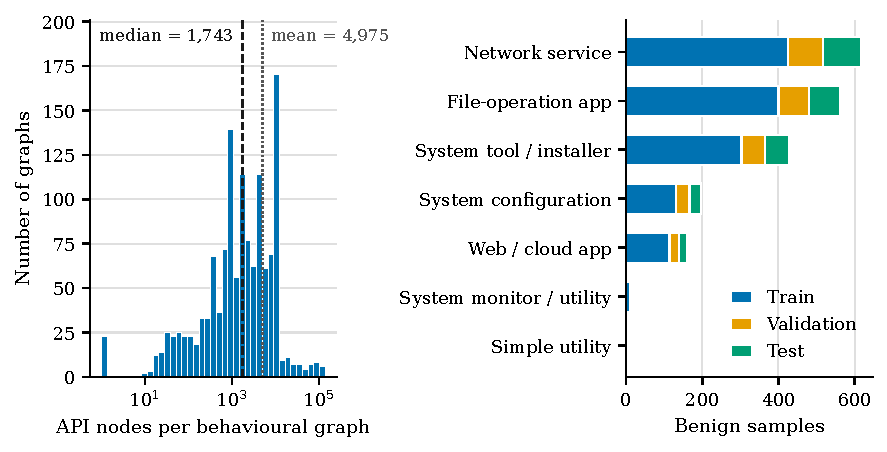
\includegraphics[width=\textwidth]{img/dataset_characterisation.pdf}
  \caption[Corpus characterisation: graph sizes and benign
  composition]{Characterisation of the evaluation corpus. Left: distribution
  of API-node counts over the 1{,}356 behavioural graphs of the validation
  split. Right: composition of the benign corpus by operational category.}
  \label{fig:dataset_characterisation}
\end{figure}

The left panel shows a heavy-tailed
size distribution: the largest trace exceeds $1.4 \times 10^{5}$ nodes and
individual samples span four orders of magnitude. The scalability mechanisms of
Section~\ref{subsec:scalability} exist for this distribution: the largest traces
are reduced rather than discarded by the behaviour-aware capping described
there. That capping is a concession to available memory, not a modelling
choice, and what it keeps are the cross-type interactions and timing spikes
that carry the model's evidence. The
right panel breaks the benign corpus down by operational category. The 1{,}987
benign samples span seven categories of legitimate software, led by network
services, file-operation applications, and system tools and installers, which
deliberately mirror the file, registry, and network activity that behavioural
threat detection must learn to tolerate. The category proportions are
consistent across the training, validation, and test splits, so no category is
concentrated in a single split, and the false-alarm figures reported in this
chapter measure the framework against the full diversity of this benign
behaviour rather than against a single software profile. The model that these
splits exist to evaluate is fixed next, and fixed once.

\subsection{Reported Model and Checkpoint Selection}
\label{subsec:exp_checkpoint}

Every result in this chapter is produced by the HeteroTemporalGNN of
Section~\ref{sec:architecture}. The framework maps an enriched heterogeneous
behavioural graph to a threat prediction through three complementary branches:
a semantic branch over pretrained MPNet API embeddings, a structural branch
formed by hybrid GAT--SAGE relational message passing, and a temporal branch
formed by a bidirectional LSTM with attention pooling. The per-sample
contributions of these branches are integrated by an adaptive gated fusion,
concatenated with graph-level behavioural statistics, and passed through a
shared fully connected trunk with a per-class output head. The bidirectional
LSTM serves as the temporal backbone throughout. The trained model comprises
approximately $16.1$ million
parameters, and a single checkpoint produces all results, so that comparisons
across experiments are not confounded by differences in model state.

The evaluated checkpoint is the one that maximised validation macro-F1 among the
training epochs that met minimum per-class recall floors on the ransomware and
benign classes. These floors prevent a checkpoint that scores well in aggregate
from being retained while under-detecting the rarest or the benign class. All
runs fix a single global random seed of $42$, and the hardware and software
environment is that of Table~\ref{tab:hw_sw_config}. What that model is measured
against is settled next.

\subsection{Baseline Configurations}
\label{subsec:exp_baseline_config}

Each baseline family introduced in Section~\ref{subsec:baselines} is instantiated
by an established method drawn from its paradigm, so that the comparison measures
the proposed representation against recognised practice rather than a
deliberately weakened baseline. Beyond the shared splits and decision rule of
Section~\ref{subsec:exp_dataset}, all four are trained on the three behavioural
classes and address class imbalance through a class-weighted loss or
class-balanced sampling rather than any alteration of the splits. Except where a
model family dictates otherwise, the neural baselines share a fixed optimisation
setup: the AdamW optimiser~\cite{loshchilov2019adamw} with a learning rate of
$10^{-3}$ and weight decay of $10^{-4}$, and a checkpoint restored from the
epoch of best validation performance. A longer schedule therefore confers no
advantage on a model that has already stopped improving. Each family's
representation and model are
specified in Table~\ref{tab:baseline_config} and described in turn below; their
internal mechanics and comparative results are deferred to
Section~\ref{sec:baseline_comparison}.

\begin{table}[htbp]
\centering
\small
\caption[Baseline family configurations]{Configuration of the four baseline families. All models are trained on
identical splits and reduced to the binary threat decision by the same argmax
projection.}
\label{tab:baseline_config}
\begin{tabular}{@{}l p{3.1cm} p{6.4cm}@{}}
\toprule
\textbf{Baseline} & \textbf{Representation} & \textbf{Model and key configuration} \\
\midrule
Classical ML &
TF-IDF unigram and bigram of the API sequence, 3000 features &
Random Forest (300 trees, no depth limit, balanced class weights) and XGBoost
(500 trees, depth 6, learning rate $0.1$) \\
\addlinespace
Sequential DL &
Learned token embeddings over the ordered API sequence &
Bidirectional LSTM (embedding 128, hidden 128, 2 layers, dropout $0.3$) with
masked attention pooling; 40 epochs, patience 8; self-contained token
vocabulary built from the training split only \\
\addlinespace
Static GNN &
The same heterogeneous graphs, static structure only &
Heterogeneous GCN and GAT (hidden 128, 2 layers; GAT with 4 attention heads);
30 epochs, patience 8; semantic API embeddings, temporal edges and timestamps,
and behavioural statistics all withheld \\
\addlinespace
Semantic-embedding &
Mean-pooled 768-dimensional MPNet API embeddings &
Multilayer perceptron ($768\rightarrow256\rightarrow128\rightarrow3$, dropout
$0.3$); 60 epochs, patience 10; reuses the cached MPNet embeddings of the
framework's semantic branch \\
\bottomrule
\end{tabular}
\end{table}

\paragraph{Classical machine learning.} Following the static feature-engineering
paradigm, the API call sequence is encoded as a TF-IDF representation of unigrams
and bigrams~\cite{salton1988tfidf} and classified by two tree ensembles, a
Random Forest~\cite{breiman2001random} and an
XGBoost~\cite{chen2016xgboost}. Reporting both a bagged and a boosted
learner represents the paradigm near its practical ceiling rather than through a
single model.

\paragraph{Sequential deep learning.} The ordered API sequence is embedded
token-by-token and encoded by a bidirectional LSTM~\cite{hochreiter1997} with
masked attention pooling~\cite{bahdanau2015attention}. Its token vocabulary is
built from the training split alone, so that any API renamed at test time is
genuinely out-of-vocabulary.

\paragraph{Static graph neural networks.} A heterogeneous
GCN~\cite{kipf2017gcn} and GAT~\cite{velickovic2018gat} are trained on the same
graphs under the withholding protocol of Table~\ref{tab:baseline_config}, so
that only static relational structure remains.

\paragraph{Semantic-embedding classification.} Mean-pooled
MPNet~\cite{mpnet2020} API embeddings are classified by a multilayer
perceptron. It operationalises the semantic-only paradigm of
BEACON~\cite{perera2023beacon}, whose zero-shot large-language-model variant
is deferred to Chapter~\ref{chap:future_work}.


\subsection{Metrics and Reproducibility}
\label{subsec:exp_metrics}

The final element of the experimental setup governs how the results themselves are
read. A figure carries meaning only under a fixed convention for how it is computed
and reported, so those conventions are settled here before any results are shown;
the metrics themselves are defined in Section~\ref{subsec:metrics}. The binary
threat decision is the primary lens, and threat recall together with the absolute count of missed
threats are treated as the headline figures, because the operational cost of the
two error types is asymmetric: a single undetected ransomware sample is far more
consequential than an isolated false alarm. The latter is reported against the
benign total of each evaluation set. Macro-averaged precision,
recall, and F1-score characterise the finer three-class behaviour beneath that
decision,
while accuracy is reported only for completeness. Unless a section states otherwise, every figure is computed
on the held-out test split defined in Section~\ref{subsec:exp_dataset}, so that
the tables that follow may be read under a single, consistent convention.

All results are moreover fully reproducible. Beyond the fixed random seed and
deterministic execution already established for the training procedure, each
experiment persists the evaluation manifest that fixes its exact sample
composition and the per-sample prediction records from which its metrics are
computed. Every figure reported below, for the proposed framework and for the
baselines alike, can therefore be regenerated exactly from the trained checkpoint
and these artefacts rather than merely re-estimated, which places the comparisons
of this chapter on a verifiable footing. With the data, model, baselines, and
reporting conventions now fixed, the evaluation opens with the framework's raw
detection performance.


\section{Threat Detection Performance}
\label{sec:main_results}

The framework is trained over three behavioural classes and deployed as a binary
threat detector. This section reports the detection performance of the reported
checkpoint on the held-out test split of $1384$ samples, comprising $39$
ransomware, $299$ benign, and $1046$ other-malware execution traces, and
establishes the two findings on which the remainder of the chapter builds: that
the framework meets the operational requirement of the detection task by
recovering every malicious sample at a modest false-alarm cost, and that the
errors it still makes fall in the direction the three-class training design
intended. The binary threat decision is examined first; the three-class
behaviour beneath it follows.

\subsection{Binary Threat Detection}
\label{subsec:binary_detection}

In practice the framework must return a single verdict, threat or not, and the
evaluation begins with that decision. The reported
checkpoint is applied once to every sample of the test split, and each
three-class prediction is projected onto the binary decision by the fixed
argmax rule of Equation~\ref{eq:binary_projection}.
Table~\ref{tab:binary_confusion} presents the resulting
threat-versus-benign confusion matrix.

\begin{table}[H]
\centering
\small
\caption{Threat-versus-benign confusion matrix on the held-out test split.}
\label{tab:binary_confusion}
\begin{tabular}{l cc c}
\toprule
 & \textbf{Predicted threat} & \textbf{Predicted benign} & \textbf{Total} \\
\midrule
Actual threat & $1085$ & $0$   & $1085$ \\
Actual benign & $16$   & $283$ & $299$  \\
\midrule
Total         & $1101$ & $283$ & $1384$ \\
\bottomrule
\end{tabular}
\end{table}

The test split contains $1085$ malicious
samples, the $39$ ransomware and $1046$ other-malware traces combined, and
the framework assigns every one of them to the threat side: no malicious sample
is classified as benign, giving a threat recall of $1.000$ and a missed-threat
count of zero. Since a missed threat, a malicious sample released as benign, is
the costliest error a detector can commit, this result establishes the property
that the remainder of the evaluation seeks to explain and to challenge: on
held-out data drawn from the same distribution as training, the framework's
threat boundary is exhaustive.

The cost of this exhaustive detection is a modest false-alarm burden. Sixteen of
the $299$ benign samples are flagged as threats, yielding a benign recall of
$0.946$ and a false-positive rate of $0.054$; threat precision is $0.985$,
threat F1-score $0.993$, and binary accuracy $0.988$. The defining property of
this operating point is that its errors fall exclusively on the conservative
side. Every mistake the model makes raises a benign sample for inspection; none
releases a threat. Under the cost asymmetry that governs the detection task, in
which a single undetected ransomware sample outweighs a small number of false
alarms, this is the appropriate direction for the residual error to take.
Figure~\ref{fig:checkpoint_selection} traces how this operating point was
reached during training.

\begin{figure}[H]
\centering
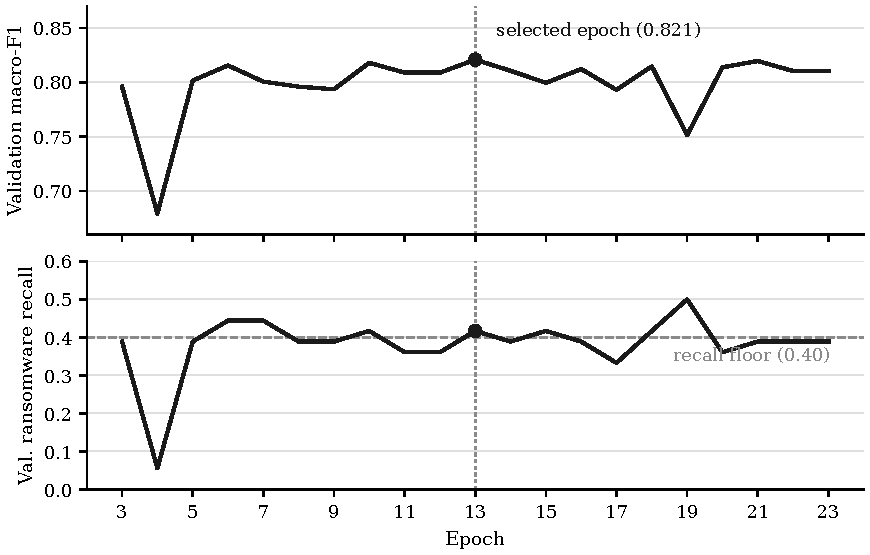
\includegraphics[width=0.95\textwidth]{img/checkpoint_selection.pdf}
\caption[Checkpoint selection on the validation split]{Checkpoint selection on the validation split over the recorded
training epochs. Top: validation macro-F1 per epoch, with the selected epoch
marked. Bottom: validation ransomware recall against the selection floor of
$0.40$; epochs below the floor are ineligible for selection regardless of their
aggregate score.}
\label{fig:checkpoint_selection}
\end{figure}

The upper panel shows validation macro-F1 over the
recorded epochs: it settles into a narrow band once training has converged, and
the selected epoch reaches the highest value, $0.821$. The lower panel shows
validation ransomware recall against the selection floor of $0.40$. Several
epochs scored competitively in aggregate, the selected epoch's closest
competitor among them, yet fell below that floor and were therefore ineligible.
The checkpoint evaluated here is the best aggregate performer among the epochs
that stayed sensitive to the rarest class, and the binary results above are its
test-split behaviour.


\subsection{Three-Class Performance}
\label{subsec:threeclass_perf}

The binary decision of Section~\ref{subsec:binary_projection} is a projection
of a finer judgement, and reading the same evaluation run before that
projection is applied shows what the coarser view absorbs. The three-class view
is markedly harder: ransomware recall is $0.462$ where the binary threat recall
was $1.000$. The two figures are consistent, because every ransomware sample
the model fails to name is still caught as other malware.
Table~\ref{tab:threeclass_metrics} reports the per-class precision, recall, and
F1-score on the test split, together with the macro averages.

\begin{table}[H]
\centering
\small
\caption[Per-class and macro-averaged test metrics]{Per-class and macro-averaged precision, recall, and F1-score of the
reported checkpoint on the held-out test split.}
\label{tab:threeclass_metrics}
\begin{tabular}{l ccc c}
\toprule
\textbf{Class} & \textbf{Precision} & \textbf{Recall} & \textbf{F1-score} & \textbf{Support} \\
\midrule
Ransomware     & $0.750$ & $0.462$ & $0.571$ & $39$   \\
Benign         & $1.000$ & $0.946$ & $0.973$ & $299$  \\
Other malware  & $0.966$ & $0.994$ & $0.980$ & $1046$ \\
\midrule
Macro average  & $0.905$ & $0.801$ & $0.841$ & $1384$ \\
\bottomrule
\end{tabular}
\end{table}

Overall three-class accuracy is $0.969$ with a macro F1-score of $0.841$. The
benign and other-malware classes are recognised almost perfectly, with
F1-scores of $0.973$ and $0.980$ respectively, and benign precision reaches
$1.000$: not a single malicious sample of either kind is assigned to the benign
class, which is the three-class restatement of the zero missed threats above.
Table~\ref{tab:threeclass_confusion} gives the corresponding confusion matrix,
which shows where the residual errors fall instead.

\begin{table}[H]
\centering
\small
\caption{Three-class confusion matrix on the held-out test split.}
\label{tab:threeclass_confusion}
\begin{tabular}{l ccc c}
\toprule
 & \textbf{Pred.\ ransomware} & \textbf{Pred.\ benign} & \textbf{Pred.\ malware} & \textbf{Total} \\
\midrule
Actual ransomware & $18$ & $0$   & $21$   & $39$   \\
Actual benign     & $0$  & $283$ & $16$   & $299$  \\
Actual malware    & $6$  & $0$   & $1040$ & $1046$ \\
\midrule
Total             & $24$ & $283$ & $1077$ & $1384$ \\
\bottomrule
\end{tabular}
\end{table}

Ransomware is, as expected, the hardest class, and the training behaviour of
the reported checkpoint shows where the difficulty originates.
Table~\ref{tab:selected_epoch_metrics} reports the per-class precision and
recall reached on the training split at the selected epoch. All three classes
are learned almost completely on the training data; in particular, the
ransomware class reaches a training recall of $0.949$ from only $172$ graphs,
$2.6\,\%$ of the split.

\begin{table}[htbp]
\centering
\small
\caption{Per-class precision and recall on the training split at the selected
epoch.}
\label{tab:selected_epoch_metrics}
\begin{tabular}{l cc}
\toprule
\textbf{Class} & \textbf{Precision} & \textbf{Recall} \\
\midrule
Ransomware    & $0.968$ & $0.949$ \\
Benign        & $0.995$ & $0.996$ \\
Other malware & $0.983$ & $0.987$ \\
\midrule
Macro F1-score & \multicolumn{2}{c}{$0.980$} \\
\bottomrule
\end{tabular}
\end{table}

This result also illustrates why ransomware was retained as a separate class.
In a binary formulation, the $172$ ransomware graphs would constitute
approximately $3.3\,\%$ of a merged threat class, and their contribution to the
classification loss would be correspondingly small. The training objective
could then be minimised through patterns shared by the majority of malware,
without learning the behaviours specific to ransomware, such as encryption
bursts and rapid mass file modification. The three-class objective assigns
these samples a separate loss term, weighted further by the focal loss and
oversampling of the training procedure, and therefore requires the model to
form a distinct ransomware representation; the training recall of $0.949$
indicates that this representation was learned. Where class scarcity does
impose a limit is at evaluation time: $172$ training graphs cannot span the
behavioural variety the class exhibits, so the learned representation
transfers only partially to unseen samples, and the test recall of $0.462$
reflects this limitation rather than a failure to learn the class.
The confusion matrix is consistent with this interpretation: all $21$
misclassified ransomware samples are predicted as other malware, the $6$ errors
in the opposite direction are malware samples predicted as ransomware, and no
sample of either malicious class is predicted as benign.

The confusion between ransomware and other malware is by design rather than by
chance. Section~\ref{subsec:binary_projection} argued that
separating ransomware from other malware during training forces the model to
learn the deeper behavioural structure of each threat type rather than a
coarse malicious-versus-benign shortcut. The mechanism is geometric: the
three-class objective encourages the model to position ransomware in its learned
representation space close to other malware, with which it shares system-level
behaviour, and far from benign activity, so that any uncertainty about a
threat's exact type resolves towards the neighbouring threat class rather
than towards benign. The test split realises exactly this behaviour: class
scarcity costs the model label granularity but not detection safety (none
released as benign), and the residual benign errors point in the same
conservative direction, with all $16$ raised as suspected malware. What the
headline result leaves open is where
this discriminative signal originates, and whether it depends on any single
branch of the architecture; the next two sections take up exactly that
question.


\section{Branch Contribution Analysis}
\label{sec:component_attribution}

The architecture of Chapter~\ref{chap:methodology} rests on a specific premise:
that malicious behaviour expresses itself jointly through the meaning of the
operations a program invokes, the relational structure of the entities it
touches, and the temporal pattern in which it acts, and that a detector should
therefore learn all three. The results of the previous section demonstrate that
the framework detects reliably, but they cannot show how it does so. A network
that had quietly learned to ignore two of its branches and route every decision
through the third would produce the same headline figures. The analysis reported
in this section was conducted to rule that possibility out, by establishing
whether each branch contributes materially to the decisions of the trained
model and how that contribution is distributed across the three behavioural
classes, the question posed by RQ2. It combines two complementary measurements.
The first silences each branch in turn and records how much confidence the
model loses without it. The second reads the fusion gate of the intact model
during unmodified inference, to see how the decisions draw on the branches
when nothing is removed. Both measurements answer the same way. Every branch
carries a material share of the decision, so none has been sidelined; the
intact model weights the three on nearly equal terms; and the branch that
leads a given decision varies with the behavioural class rather than
following a fixed hierarchy.

\subsection{Branch Contribution Shares}
\label{subsec:branch_contributions}

The first of these two measurements examines each branch through targeted
silencing, which gauges its branch share as the cost of its
absence. Since the three branches feed a single fused representation, the
influence of any one of them cannot be isolated from the prediction of the
intact model; it is exposed by disabling the branch and re-evaluating the same
sample on the remaining two. Each sample is therefore passed through the
trained model four times: once intact, and once with each branch disabled in a
way that leaves the rest of the forward pass valid. The
semantic branch is silenced by zeroing the pretrained embedding block of the
API node features, the structural branch by removing the non-temporal relations
from the graph while preserving a minimal executable backbone, and the temporal
branch by suppressing the output of the recurrent encoder. Each variant yields
a drop in the confidence of the originally predicted class relative to the
intact run; a large drop means the silenced branch supplied information the
remaining branches could not reproduce, and a negligible drop means they could
carry the decision without it. The three drops are then normalised to shares summing to
one, so that each share measures how far the other two fall short of replacing
that branch. The attribution was run over $300$-sample subsets of
the training and test splits, $600$ samples in total, selected in hash order of
the sample identifiers, which is independent of class and behaviour.
Table~\ref{tab:branch_contributions} reports the shares averaged per class on
the test subset, the averages of each split, and the overall average across all
attributed samples.

\begin{table}[H]
\centering
\caption[Branch contribution shares]{Contribution shares from leave-one-branch-out attribution. The upper
block resolves the test subset by class; the lower block averages each
$300$-sample split and all $600$ attributed samples. Each share measures how far
the other two branches fall short of replacing it.}
\label{tab:branch_contributions}
\begin{tabular}{l r ccc}
\toprule
 & \multicolumn{1}{c}{$n$} & \textbf{Semantic} & \textbf{Structural} & \textbf{Temporal} \\
\midrule
\multicolumn{5}{l}{\textit{Test subset, by class}} \\
Ransomware    & $13$  & $44.7\,\%$ & $15.0\,\%$ & $40.3\,\%$ \\
Benign        & $63$  & $49.8\,\%$ & $10.4\,\%$ & $39.8\,\%$ \\
Other malware & $224$ & $62.9\,\%$ & $15.1\,\%$ & $22.0\,\%$ \\
\midrule
\multicolumn{5}{l}{\textit{By split, all classes}} \\
Training      & $300$ & $59.9\,\%$ & $28.2\,\%$ & $11.9\,\%$ \\
Test          & $300$ & $59.3\,\%$ & $14.1\,\%$ & $26.5\,\%$ \\
\midrule
All samples   & $600$ & $59.6\,\%$ & $21.2\,\%$ & $19.2\,\%$ \\
\bottomrule
\end{tabular}
\end{table}

Three observations follow from the table. First, no branch is redundant:
silencing any one of them costs a double-digit share for every class of the
test subset, so the fusion does not reduce to a single pathway with two
passengers. Second, the composition of the shares is class-dependent. The
semantic branch carries the largest share overall and is clearest for other
malware, where silencing it costs $62.9\,\%$ of the measured total and it is
the dominant contributor for $183$ of the $224$ samples, consistent with the
breadth of API vocabulary that distinguishes malware families. Ransomware draws
almost equally on the semantic and temporal branches ($44.7\,\%$ and
$40.3\,\%$), and the temporal branch is the single largest contributor for $8$
of its $13$ samples, in keeping with the class's characteristic execution
signature of encryption bursts and rapid mass file modification. Benign
software shows the same semantic and temporal pairing ($49.8\,\%$ and
$39.8\,\%$, with the dominant contributor split evenly between the two
branches), indicating that ordinary software is recognised by what its
operations mean and by its unhurried pacing, while its structural share under
silencing is the smallest in the table at $10.4\,\%$.

Third, the composition is also sample-dependent: on the training subset the
structural share is twice its test-subset value ($28.2\,\%$ against
$14.1\,\%$), with the temporal share moving in the opposite direction. The
splits are stratified by class, so this is not a shift in class composition.
This variation is not an inconsistency but the behaviour
the adaptive design is intended to produce: which branch the other two cannot
replace follows the behavioural evidence present in the samples at hand rather
than a fixed template applied uniformly. Averaged over all $600$ attributed
samples, the shares settle at $59.6\,\%$ semantic, $21.2\,\%$ structural, and
$19.2\,\%$ temporal. The experiment therefore delivers the outcome the
architecture was designed for, and with it the answer to the first half of the
section's question: no branch is dispensable, each supplies something the other
two cannot, and the mixture varies with both the class and the samples being
explained rather than being routed through a single branch.

The prominence of the semantic branch in this table should not be read as
semantics alone driving the framework's decisions. A share measures how
replaceable a branch is, not how much the model uses it. The semantic branch's
share is large precisely because the
information it carries is unique: the meaning of an API call exists nowhere
else in the representation, so when the embeddings are silenced the structural
and temporal views cannot reconstruct what was lost. How much the model
actually leans on each branch in forming a decision cannot be read from a table
of removals.

\subsection{Adaptive Reliance Across Classes}
\label{subsec:branch_specialisation}

The previous measurement gauged a branch by its absence; this one reads the
model while it is intact and undisturbed, taking the weighting it assigns to
the three branches at the moment it decides. That weighting is produced by the
adaptive gated fusion of Section~\ref{subsec:fusion}, in which a gating network
reads the pooled representations of the three branches and produces a
normalised weight triple for each sample, and the fused representation from
which the classification is made is the sum of the branch representations
scaled by exactly these weights. A branch's gate weight is therefore a direct
measure of how strongly its view enters that sample's decision, and since the
triples are produced on every forward pass, whether the deciding is
concentrated in one branch or shared across all three can be read from them
without altering the model's behaviour. The weight triples were logged for each
of the $440$ samples scored in the evaluation of
Section~\ref{sec:generalisation_results}, the $330$ held-out samples of the
primary corpus together with the $110$ threats from the unseen source;
Table~\ref{tab:gate_weights} reports their means by true class, and
Figure~\ref{fig:branch_usage} visualises them together with how often each
branch receives the largest weight. Averaged over all samples the gate is
nearly uniform, at $0.354$, $0.353$, and $0.293$ for the semantic, structural,
and temporal branches respectively, so the fusion does not collapse onto a
preferred branch. The per-class view, however, shows that this balance is an
average over strongly class-adaptive behaviour rather than a static compromise.

\begin{table}[htbp]
\centering
\caption[Mean gate weights by true class]{Mean adaptive-fusion gate weights by true class, recorded at inference
with nothing silenced. The gate weight measures how much the intact model draws
on each branch when forming a decision.}
\label{tab:gate_weights}
\begin{tabular}{l r ccc}
\toprule
\textbf{Class} & \multicolumn{1}{c}{$n$} & \textbf{Semantic} & \textbf{Structural} & \textbf{Temporal} \\
\midrule
Ransomware    & $75$  & $0.661$ & $0.130$ & $0.209$ \\
Benign        & $200$ & $0.223$ & $0.450$ & $0.327$ \\
Other malware & $165$ & $0.374$ & $0.337$ & $0.289$ \\
\midrule
All samples   & $440$ & $0.354$ & $0.353$ & $0.293$ \\
\bottomrule
\end{tabular}
\end{table}


The per-class rows of Table~\ref{tab:gate_weights} show this adaptation
directly. For ransomware the gate concentrates on the semantic branch with a
mean weight of $0.661$; for benign software it shifts to the structural branch
($0.450$), indicating that the relational shape of ordinary system activity is
what most cleanly separates it from threats; for other malware the weights
remain close to uniform ($0.374$, $0.337$, $0.289$).
Figure~\ref{fig:branch_usage} presents the same measurements graphically and
adds a view the means cannot provide.

\begin{figure}[H]
\centering
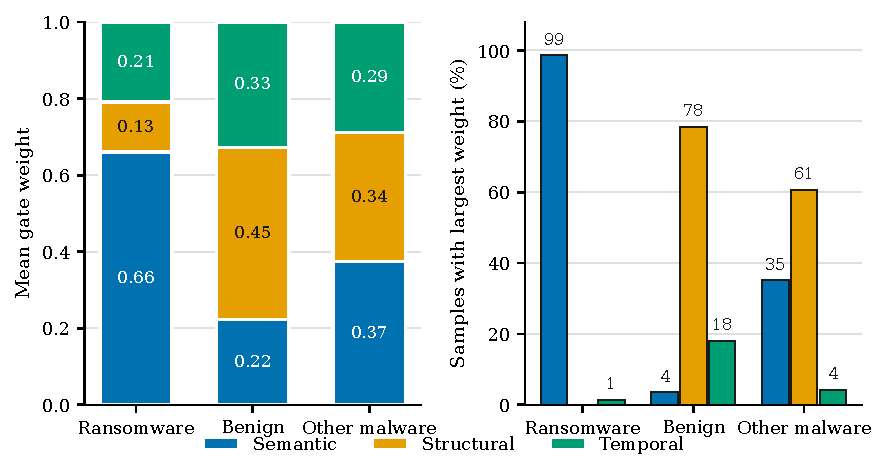
\includegraphics[width=\textwidth]{img/branch_usage.pdf}
\caption[Adaptive branch usage by true class]{Adaptive fusion behaviour by true class, recorded with the reported
checkpoint. Left: mean gate weight assigned to each branch. Right: percentage
of samples in which each branch receives the largest weight.}
\label{fig:branch_usage}
\end{figure}

The left panel stacks the per-class mean
weights of the table; the right panel counts, for each class, how often each
branch receives the largest weight of a sample's triple, which distinguishes a
branch that typically leads a decision from one that holds a steady minority
stake. These dominance counts sharpen the class pattern: the semantic branch
leads in $98.7\,\%$ of ransomware decisions and the structural branch in
$78.5\,\%$ of benign decisions, while for other malware the semantic branch
holds the higher mean weight but the structural branch leads more often
($60.6\,\%$ against $35.2\,\%$), a combination that is only possible because
the gate re-weights every sample individually rather than applying a fixed
template per class.

Set against Table~\ref{tab:branch_contributions}, the two instruments agree
that semantics leads on both threat classes but diverge on the benign class,
and the divergence is informative because the two ask different questions. The
gate asks how much the model draws on a branch while deciding; the shares ask
how much would be lost if it could not. Benign software is the clearest case.
The gate routes benign decisions primarily through the structural branch
($0.450$), yet silencing that branch costs benign predictions the smallest
share of support in the table ($10.4\,\%$). Structure therefore guides how a
benign decision is formed, while the evidence it contributes can largely be
reconstructed from the other two branches. The semantic branch shows the
opposite pattern on the benign and other-malware classes, its contribution
share exceeding its gate weight ($49.8\,\%$ against $0.223$ on benign samples)
because the information it supplies is the least substitutable. Read together,
the two instruments assign the branches consistent roles: semantics identifies
which threat is being observed, structure organises the recognition of benign
behaviour, and the temporal branch supplies a steady supporting signal that
becomes co-primary precisely for the classes whose behaviour is defined by
pacing.

The silencing and gating results together confirm the premise this section set
out to test. In the intact model the three branches participate in the decision
on almost equal terms;
every branch carries a material share of the decision support when silenced,
and which branch leads a decision depends on the behavioural class rather than
on a fixed hierarchy. Both measurements, however, operate at the level of
individual decisions: they quantify confidence and attention, and so establish
that every branch is genuinely used, but not what the framework would still
detect if a branch were lost. The next section therefore moves from explanation
to stress test: entire branches are removed outright, and the detection
performance itself, threat recall and the count of missed threats, is
re-measured in their absence.


\section{Ablation Study}
\label{sec:ablation_results}

An ablation study measures the importance of a component through the cost of
doing without it. The trained model is re-evaluated with one component
deliberately disabled while everything else, the learned weights, the
evaluation data, and
the decision rule, is held fixed; the performance that disappears is
attributed to the absent component, and the performance that remains measures
how well the surviving components compensate for it. The technique is the
natural counterpart to the attribution analysis of
Section~\ref{sec:component_attribution}: attribution explained how the intact
model distributes its reliance across the semantic, structural, and temporal
branches, whereas ablation establishes what the framework can still detect
once a branch is genuinely gone. The two questions are not interchangeable,
because a model may spread its attention broadly yet collapse the moment a
single input fails, or conversely conceal substantial redundancy behind
specialised averages. The objective of this experiment is therefore to
establish whether the branch contributions documented so far are redundant
enough for detection to survive the loss of any one of them, and to
characterise what kind of error such a loss produces.

This distinction carries the remaining weight of RQ2. Each branch depends on
a signal that can degrade in practice: the semantic branch needs API names to
mean what they say, the structural branch needs a visible interaction topology,
and the temporal branch needs the execution order intact. A detector hinging
on any one of them has a single point of failure.

The study reuses the evaluation machinery of
Section~\ref{sec:component_attribution}: the same sample of 300 test graphs,
comprising 237 threats and 63 benign applications, and the same three
silencing mechanisms, so that any difference in conclusions stems from what is
measured rather than from how. What is measured, however, changes. Where
attribution recorded shifts in prediction confidence, the quantities read
here are detection outcomes: the number of threats missed, the number of
false alarms raised, and the exact-class accuracy of the surviving model.
Every changed prediction is resolved by direction. The analysis proceeds at
two granularities. Whole branches are removed first, singly and in pairs; the
removals then descend into the branches themselves, targeting individual edge
relations, timestamp integrity, and embedding content. Two findings emerge.
Threat
detection survives the outright loss of any single branch, with the worst
case retaining 95.8\% threat recall, and the errors that each removal
introduces are branch-specific, falling predominantly on the conservative
side of the decision.

\subsection{Branch Removal}
\label{subsec:branch_removal}

The branch level of the study puts the single-point-of-failure question
directly to the architecture, and it does so at two complementary strengths
so that tolerance and self-sufficiency are measured separately. In the
\emph{drop-one} configurations a single branch is silenced and the remaining
two carry the decision, which measures how well the model tolerates the
loss of each information source in the presence of the others. In the
\emph{keep-one} configurations two branches are silenced simultaneously and a
single branch operates alone, which measures the standalone detection
competence that each branch retains without any support. Both strengths
re-evaluate the same 300 graphs under the mechanisms described in
Section~\ref{subsec:branch_contributions}, and each configuration is compared
against the intact model, which misses none of the 237 threats, raises four
false alarms, and assigns the exact class to 285 of the 300 samples.
Table~\ref{tab:branch_removal} reports all six ablated configurations
against this reference.

\begin{table}[H]
\centering
\caption[Branch-removal ablation results]{Detection outcomes of the
branch-removal ablations on the 300-graph test sample (237 threats, 63
benign). Drop-one rows silence a single branch; keep-one rows retain a single
branch and silence the other two. A missed threat is a threat sample
reassigned to the benign class; a false alarm is a benign sample assigned to
a threat class.}
\label{tab:branch_removal}
\begin{tabular}{l c c c c}
\toprule
Configuration & \makecell[c]{Threats missed\\(of 237)} & Threat recall &
\makecell[c]{False alarms\\(of 63)} & \makecell[c]{Exact class\\(of 300)} \\
\midrule
Intact model      & 0  & 1.000 & 4  & 285 \\
\addlinespace
No semantic       & 0  & 1.000 & 15 & 228 \\
No structural     & 10 & 0.958 & 1  & 278 \\
No temporal       & 1  & 0.996 & 4  & 284 \\
\addlinespace
Semantic only     & 8  & 0.966 & 2  & 279 \\
Structural only   & 0  & 1.000 & 10 & 259 \\
Temporal only     & 8  & 0.966 & 17 & 233 \\
\bottomrule
\end{tabular}
\end{table}

The drop-one rows establish the tolerance directly, and the most instructive
of them concerns the semantic branch. Section~\ref{sec:component_attribution}
identified it as the largest single contributor to the model's confidence,
yet silencing it misses not one of the 237 threats. Its loss registers
elsewhere: eleven additional benign applications cross to the threat side,
and exact-class accuracy falls from 285 to 228 correct samples, by far the
largest drop of any single removal. Without semantics the model still
recognises that a sample behaves maliciously, but it becomes less certain
about which malicious class the behaviour belongs to and more suspicious of
legitimate software, an error profile that degrades precision and analyst
workload rather than safety. Silencing the structural branch inverts this
profile. It is the only single-branch removal that produces a material number
of missed threats, ten, while false alarms fall from four to one; the
structural view is what pushes borderline samples towards the threat side, so
its absence makes the model both less alarm-prone and less
threat-sensitive. Silencing the temporal branch costs a single missed threat
and one exact-class error, the smallest footprint of the three, consistent
with its role in Section~\ref{sec:component_attribution} as the branch that
supports decisions more often than it leads them.

The keep-one rows subject the architecture to a far harsher condition than
any realistic degradation, and detection still does not collapse. The
structural branch operating alone recovers every one of the 237 threats at
the price of ten false alarms, making it the most dependable standalone
threat alarm of the three. The semantic branch alone misses eight threats but
retains the best exact-class accuracy of the keep-one rows, 279 of 300,
confirming that its speciality is naming the behaviour rather than merely
flagging it. The temporal branch alone is the weakest keep-one
configuration, with eight missed threats and seventeen false alarms, yet even
this most degraded form of the framework still detects 96.6\% of the threats it
faces. Each branch
can carry the binary decision after a fashion, but none reproduces the intact
model. Degradation is therefore graceful rather than harmless.
Figure~\ref{fig:branch_removal} juxtaposes the two failure
dimensions across all seven configurations.

\begin{figure}[H]
  \centering
  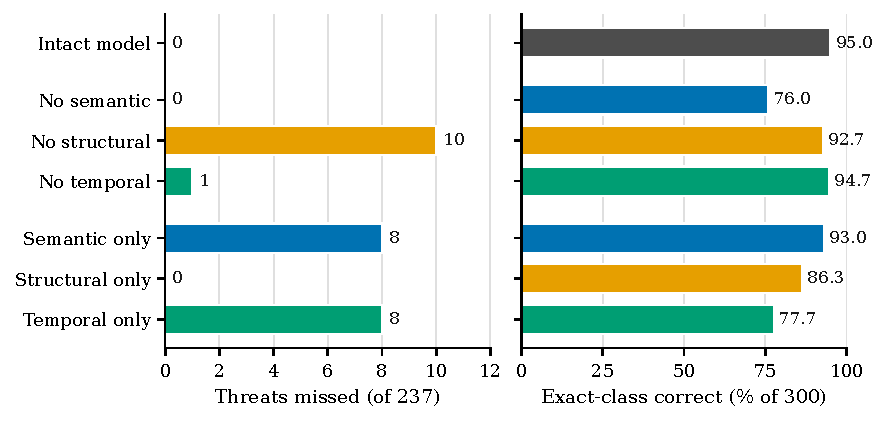
\includegraphics[width=\textwidth]{img/branch_removal.pdf}
  \caption[Branch-removal ablation: missed threats and exact-class
  accuracy]{Detection outcomes across the seven branch configurations of
  Table~\ref{tab:branch_removal}. Left: threats missed out of 237. Right:
  exact-class accuracy over the 300-graph sample. Bars are coloured by the
  branch each configuration concerns; the intact reference is grey.}
  \label{fig:branch_removal}
\end{figure}

The left panel shows how narrowly the missed-threat
count is concentrated: it moves materially only when the structural branch is
absent, in the no-structural and the two structure-less keep-one
configurations, and stays at or near zero everywhere else. The right panel
shows the complementary pattern: exact-class accuracy is governed almost
entirely by the semantic branch, with every configuration lacking it scoring
below every configuration that retains it. Read together, the panels separate the
two failure axes, and the reason lies in what each decision needs: judging a
sample malicious needs only that its interactions look abnormal, which
structure supplies without naming any call, while naming the threat needs the
operations themselves, which only the embeddings carry.

These results also resolve the question that
Section~\ref{sec:component_attribution} deliberately left open. The branch
with the largest contribution share is the one whose removal misses nothing,
which demonstrates that contribution and indispensability are genuinely
different properties: the semantic branch contributes more to the model's
confidence than either other branch, yet the information it carries about the
threat decision, though not about the class decision, is recoverable from the
other two views. The
branches therefore overlap on the binary question, which is what allows
detection to degrade gracefully, and specialise beyond it, which is why only
the full model reaches 285 of 300 exact classifications while no single
branch exceeds 279. This is the complementary-but-redundant behaviour the
architecture was designed to exhibit, observed here by silencing branches
rather than inferred from the intact model.

A branch, however, has several distinct constituents. The second stage of the
study therefore targets one constituent of the branch at a time rather than
the whole of it.

\subsection{Relation and Feature-Level Ablations}
\label{subsec:relation_feature_ablation}

The ten ablations of this stage reach inside the branches, each removing or
perturbing one relation or feature while the rest of the model stays intact.
The cost measured for a whole branch can then be traced to the part that
produced it. The structural
branch reasons over typed edge relations, so each relation is removed in turn
while the others remain: the process-to-API
anchoring edges, the three context relations linking API calls to file,
registry, and network entities, and the temporal-ordering edges between
consecutive API events. The temporal branch consumes recorded timestamps
together with the temporal edge features engineered from them, so the
integrity of the timestamps is perturbed in three ways: shuffling
them, reversing them, and collapsing them to a single instant. The semantic branch
consumes pretrained embedding vectors, whose content is corrupted at two
intensities short of the outright zeroing already measured: shuffling the
embedding dimensions and overwriting the vectors with Gaussian noise. Each of
the ten ablations re-evaluates the same 300 graphs, and
Table~\ref{tab:relation_feature_ablation} reports the mean confidence drop
alongside the direction-resolved detection outcomes.

\begin{table}[htbp]
\centering
\caption[Relation- and feature-level ablation results]{Relation- and
feature-level ablations on the 300-graph test sample. The mean confidence
drop is the average absolute change in predicted-class confidence; decisions
changed counts samples whose predicted class differs from the intact
prediction. The intact model raises four false alarms, so values of four in
the final column indicate no benign-side movement.}
\label{tab:relation_feature_ablation}
\small
\setlength{\tabcolsep}{4.5pt}
\begin{tabular}{l c c c c}
\toprule
Ablation & \makecell[c]{Confidence\\drop} & \makecell[c]{Decisions\\changed} &
\makecell[c]{Threats missed\\(of 237)} & \makecell[c]{False alarms\\(of 63)} \\
\midrule
\multicolumn{5}{l}{\emph{Structural relations}} \\
Process$\to$API edges removed   & 0.060 & 13 & 10 & 1 \\
API$\to$file edges removed      & 0.001 & 0  & 0  & 4 \\
API$\to$registry edges removed  & 0.000 & 0  & 0  & 4 \\
API$\to$network edges removed   & 0.000 & 0  & 0  & 4 \\
Temporal edges removed          & 0.025 & 5  & 0  & 5 \\
\addlinespace
\multicolumn{5}{l}{\emph{Temporal features}} \\
Timestamps shuffled             & 0.010 & 2  & 0  & 4 \\
Timestamps reversed             & 0.007 & 0  & 0  & 4 \\
Timestamps collapsed            & 0.000 & 0  & 0  & 4 \\
\addlinespace
\multicolumn{5}{l}{\emph{Semantic content}} \\
Embedding dimensions shuffled   & 0.015 & 2  & 0  & 4 \\
Embeddings noise-corrupted      & 0.072 & 16 & 0  & 5 \\
\bottomrule
\end{tabular}
\end{table}

The structural block localises the branch-level finding sharply. Removing
only the process-to-API relation reproduces the entire structural ablation of
Table~\ref{tab:branch_removal}: the same ten missed threats and the same
single false alarm, with a mean confidence drop of $0.060$ matching the
branch-level removal to three decimal places. The
three context relations, by contrast, can each be removed without changing a
single decision. The structural signal that detection depends on is therefore
not distributed across the graph topology but concentrated in the relation
that anchors every API event to the process issuing it; the file, registry,
and network relations are individually redundant, their discriminative
content evidently recoverable from the API identities themselves and from the
remaining views. Removing the temporal-ordering edges sits between these
extremes, changing five decisions without costing a threat, since it removes
only one of the two routes by which timing reaches the decision.

The temporal block explains a subtlety the branch-level results could not, and
it is one the architecture was built to produce. Silencing the temporal branch
outright costs a missed threat and a measurable confidence drop, yet reordering
the sequence it reads costs almost nothing: shuffling the order changes two
decisions, reversing it changes none, and collapsing every event to one
instant changes none either. The reason lies in the design of
Section~\ref{subsec:temporal_branch}, where the engineered temporal edge
features are folded into the API node states during message passing, so every
state carries the pacing of execution before the sequence model sees it. The
ordering imposed by the recurrent pass is therefore a second reading of
evidence the node states already hold rather than the sole carrier of it, and
timing held in two places at once does not fail when one of them is disturbed.
That redundancy is deliberate, and the branch earns its place even so, since
silencing it outright still costs a threat.

The semantic block completes a gradient that runs across both tables.
Shuffling the embedding dimensions changes two decisions, corrupting the
vectors with noise changes sixteen, and zeroing them outright, the
branch-level ablation, changes sixty-nine: the impact scales with how much of
the embedding content is destroyed. Yet the number of missed threats
remains zero at every intensity, zeroing included. Within this table the
corruptions move samples between the two threat classes and push at most one
benign sample across the decision boundary, never converting a threat into a
benign verdict, reinforcing the branch-removal finding that the binary
decision does not rest on semantics alone.

\begin{figure}[H]
  \centering
  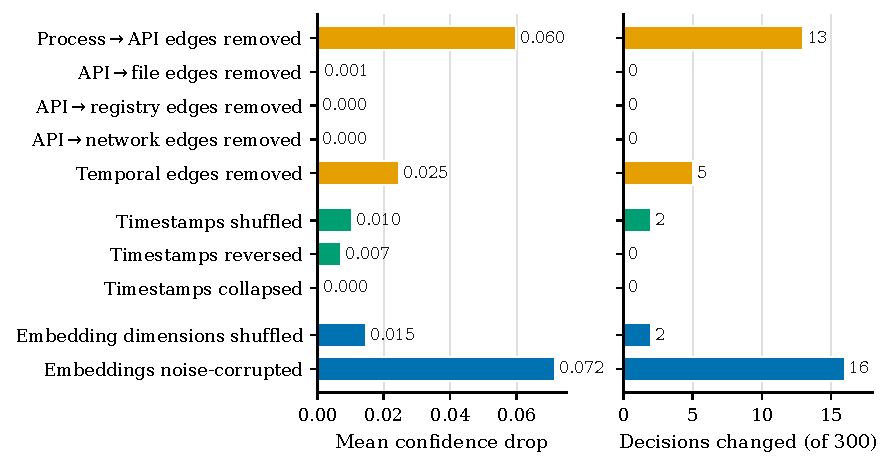
\includegraphics[width=\textwidth]{img/fine_ablation.pdf}
  \caption[Relation- and feature-level ablation effects]{Effect of the ten
  relation- and feature-level ablations of
  Table~\ref{tab:relation_feature_ablation}. Left: mean confidence drop.
  Right: decisions changed out of 300.}
  \label{fig:fine_ablation}
\end{figure}

Figure~\ref{fig:fine_ablation} places the ten ablations side by side, coloured
by the branch each targets, and makes the asymmetry between the branches
immediately visible, one bar dominating each block that matters and the
temporal block barely registering at all. Set against each other, the two
panels show that confidence movement does not translate into decision changes
one for one. Reversing the timestamps
moves confidence without changing a single decision, which shows that the
decision margins established by the intact model absorb moderate perturbation
before any prediction flips. Read together, the panels condense
this level of the study into one finding: the signal each branch depends on is
narrow, and nothing the temporal branch consumes can be perturbed into a
missed threat.

The two levels of the study together answer RQ2, the complementarity question
posed at its outset, and they do so in combination with the preceding section
rather than in isolation. Section~\ref{sec:component_attribution} established that the
intact model genuinely uses all three branches, with near-equal mean gate
weights and class-dependent leadership; this section established that the
threat decision survives the loss of any one of them, the worst single-branch
removal still retaining 95.8\% threat recall, while no branch on its own
reaches the full model's exact-class accuracy; the finer level traced that
dependency to a single relation, the process-to-API anchoring, the only
constituent whose removal costs a threat. These are two different facts
about the same architecture, and
both are required. If the model used all three branches heavily but each
carried unique information, the loss of any branch would collapse detection;
if the branches merely duplicated one another, two of them would contribute
nothing to the intact model. The measurements exclude both cases.

The keep-one results point beyond this section. A model left with one branch
is close to a single-paradigm detector: the semantic branch alone works like
an embedding classifier, the structural branch alone like a static graph
model, and the temporal branch alone like a sequence model. The resemblance
is only a hint, because each branch was trained alongside the other two
rather than on its own, so it cannot stand in for a detector built that way
from the start. Section~\ref{sec:baseline_comparison} makes that comparison
properly, against the four baseline families of
Section~\ref{subsec:exp_baseline_config}, each built and trained as a
detector in its own right.

One doubt about the intact model remains before that external comparison,
and it concerns the branch this chapter has scrutinised most. The semantic
branch carries the largest contribution share of
Section~\ref{sec:component_attribution}, and this section has shown that its
loss is survivable; neither measurement, however, says anything about the
quality of the signal while the branch is present. A branch that had merely
memorised the embedding vectors encountered during training would produce
exactly the tables reported here, because a memorised signal and an
understood one are damaged identically when meaning is destroyed. Whether the
semantic branch has learned what API behaviour means, or has overfitted to the
identities it was trained on, requires a different intervention: substituting
the semantic content with its meaning preserved. The next section performs that
substitution and establishes that the framework neither over-relies on its
semantic view nor reduces it to memorised identities.


\section{Semantic Robustness}
\label{sec:robustness_results}

Among the three branches, the semantic one invites a suspicion that the
preceding sections cannot dispel. Its input is produced by a pretrained
sentence-transformer encoder, and
Section~\ref{sec:component_attribution} showed that it carries the largest
share of the intact model's confidence; a component of this kind can earn
such a contribution in two very different ways. The model may genuinely
understand what an operation means, or it may have memorised the particular
embedding identities encountered during training, an overfitted shortcut
that scores well on familiar data and fails the moment the vocabulary
shifts. This section settles the question by proving two claims: that
detection is not overdependent on the semantic view, and that what the
branch contributes is learned understanding of API behaviour rather than
memorised identity, the property RQ1 demands.

Switching the branch off cannot tell understanding from memorisation, since
both are lost when it goes. Substituting equivalent vectors can, because only
memorisation breaks. Following the semantic-vector track of
Section~\ref{subsec:robustness_eval}, every semantic API embedding in a graph
is replaced at evaluation time under two contrasted regimes: by that of the
operation's nearest functional neighbour, which preserves meaning while
changing identity, and by that of another operation drawn at random from the
same trace, which destroys it. A branch that memorised identities is damaged
equally by both; one that reads meaning tolerates the first and is hurt only
by the second. The substitution applies to at least 96\% of the graphs in
every subset, so no outcome can be attributed to a residue of untouched
vectors.

The examination proceeds in two stages. The first applies the substitution to
the intact model (Section~\ref{subsec:semantic_sub_intact}), which tests
overdependence. The second applies it with the structural pathway silenced
(Section~\ref{subsec:semantic_sub_no_structure}), which tests memorisation,
because structure can then no longer compensate. The intact model barely
notices the substitution. Only when it must rely on the branch do the two
regimes separate, and then losing meaning costs several times more than losing
identity alone.

\subsection{Substitution in the Intact Model}
\label{subsec:semantic_sub_intact}

The overdependence claim is tested first, on the framework exactly as it
would be deployed. The question is whether the detection performance
established in Section~\ref{sec:main_results} is tied to the specific
semantic vectors the model was trained with: if it is, replacing them at
inference time must destabilise the predictions, and if the framework
genuinely balances its three views, the corruption of one view should be
absorbed by the other two.

The trained checkpoint is evaluated on sampled subsets of the three data
partitions, 300 training, 100 validation, and 400 test graphs, first clean
and then with each substitution regime applied to the same graphs. Every
perturbed prediction is compared with the same sample's clean prediction, so
each measurement is a paired reading, and prediction changes are resolved by
direction as in the preceding sections.
Table~\ref{tab:semantic_sub_intact} reports classification quality and
missed threats under the three conditions.

\begin{table}[htbp]
\centering
\caption[Semantic-vector substitution in the intact model]{Effect of
near-total semantic-vector substitution on the intact model. Semantic
substitution replaces each API embedding with that of its nearest functional
neighbour; random substitution replaces it with that of another operation
drawn at random. Threat counts per subset: 219 (train), 77 (validation), 306
(test).}
\label{tab:semantic_sub_intact}
\small
\begin{tabular}{l c c c c c c c}
\toprule
& & \multicolumn{3}{c}{Macro-F1} & \multicolumn{3}{c}{Threats missed} \\
\cmidrule(lr){3-5} \cmidrule(lr){6-8}
Split & Samples & Clean & Semantic & Random & Clean & Semantic & Random \\
\midrule
Train      & 300 & 0.798 & 0.787 & 0.750 & 9 & 9 & 9 \\
Validation & 100 & 0.758 & 0.758 & 0.739 & 0 & 0 & 0 \\
Test       & 400 & 0.794 & 0.791 & 0.779 & 1 & 2 & 2 \\
\bottomrule
\end{tabular}
\end{table}

The movement in Table~\ref{tab:semantic_sub_intact} barely rises above
measurement noise. Macro-F1 changes by at most 0.011 under meaning-preserving
substitution and by at most 0.048 under random substitution, and the binary
decision hardly registers the intervention at all: the test subset misses one
threat of 306 clean and two under either regime, while the training and
validation subsets record no change in missed threats whatsoever. Replacing
effectively the entire semantic input of the model therefore costs the
deployed framework almost nothing on the decision it exists to make, which
is the overdependence claim answered: no reliance on exact semantic
identities is observable at the level of detection outcomes.

This stability follows from the fusion design. The adaptive gate re-weights
the three branches for every sample, so when the semantic evidence turns
unreliable the structural and temporal views carry the decision; it is the
same redundancy that Section~\ref{sec:ablation_results} measured under
outright removal, observed here under corruption instead.
Figure~\ref{fig:semantic_sub_intact} adds the paired measures that
Table~\ref{tab:semantic_sub_intact} does not report.

\begin{figure}[H]
  \centering
  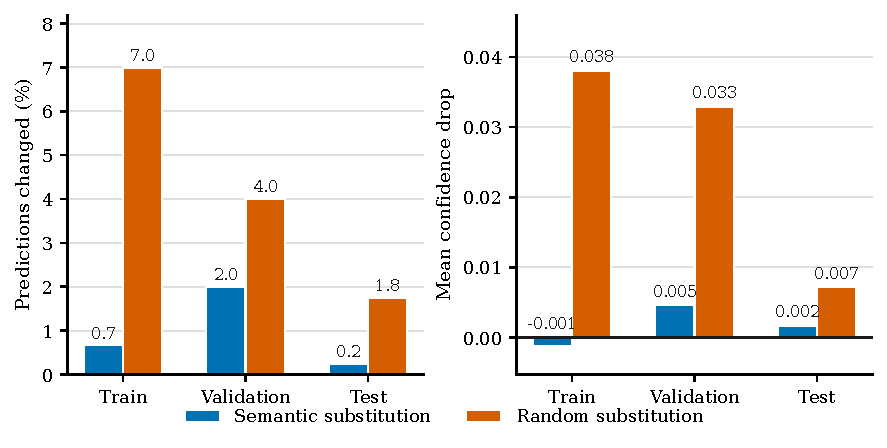
\includegraphics[width=\textwidth]{img/semantic_substitution.pdf}
  \caption[Semantic-vector substitution: paired effects on the intact
  model]{Paired effects of the two substitution regimes on the intact model.
  Left: proportion of predictions that change relative to clean evaluation.
  Right: mean confidence drop on originally correct predictions.}
  \label{fig:semantic_sub_intact}
\end{figure}

The left panel of Figure~\ref{fig:semantic_sub_intact} shows that even where
aggregate scores stay flat, the two regimes do not act alike. Random
substitution changes more predictions than meaning-preserving substitution on
every split, 1.8\% against 0.3\% on the test subset and 7.0\% against 0.7\%
on the training subset. The right panel repeats the pattern in confidence.
Destroying meaning depresses the confidence of originally correct predictions
by up to 0.038, while exchanging identities moves it by at most 0.005. On the
training subset it leaves confidence marginally \emph{higher} than clean
evaluation. Already in the intact model, then, the response tracks what a
substitution does to meaning rather than the mere fact that the vectors
changed, a first indication of the property the section is after.

The indication is not proof that the branch reads meaning, because the
stability has a second possible cause.
Section~\ref{sec:ablation_results} established that detection survives with
the semantic branch silenced outright, so a model that simply discounted its
corrupted semantic input and leaned on the remaining views would produce
exactly the flat figures above. A branch that withstands corruption and a
branch the model can do without are observationally identical while the other
views stand ready to compensate. Separating them requires an evaluation in
which the model cannot fall back on structure, and constructing that
evaluation is the purpose of the second experiment.

\subsection{Substitution without Structural Support}
\label{subsec:semantic_sub_no_structure}

Forcing the model to rely on the branch under test resolves the ambiguity.
In this experiment the structural pathway is silenced through the same
edge-removal mechanism as in the ablation study, so every decision must be
carried by the semantic and temporal views, and the two substitution regimes
are then applied on top of this weakened configuration. The discriminating
prediction is fixed before the data are read: if the semantic branch
memorised its training vectors, synonym and random replacement are equally
foreign to it and must damage detection equally; if it reads meaning, the
synonym replacement should cost little and only the destruction of meaning
should register.

Four tracks are evaluated on an independently drawn sample of 300 held-out test
graphs, comprising 226 threats and 74 benign applications: the intact model, the no-structure model, and the
no-structure model under each of the two substitution regimes, at the same
near-total substitution fraction as before.
Table~\ref{tab:semantic_sub_no_structure} reports them.

\begin{table}[htbp]
\centering
\caption[Substitution under forced semantic reliance]{Semantic-vector
substitution with the structural pathway silenced, on 300 held-out test
graphs (226 threats, 74 benign). The substitution regimes are applied on top
of the no-structure configuration.}
\label{tab:semantic_sub_no_structure}
\small
\setlength{\tabcolsep}{4pt}
\begin{tabular}{l c c c c}
\toprule
Track & Accuracy & Macro-F1 & \makecell[c]{Threats missed\\(of 226)} &
\makecell[c]{False alarms\\(of 74)} \\
\midrule
Clean                        & 0.983 & 0.861 & 0  & 1 \\
No structure                 & 0.960 & 0.840 & 8  & 0 \\
No structure + semantic sub. & 0.953 & 0.835 & 10 & 0 \\
No structure + random sub.   & 0.907 & 0.724 & 21 & 0 \\
\bottomrule
\end{tabular}
\end{table}

The first two rows of Table~\ref{tab:semantic_sub_no_structure} reproduce
what is already known: intact, the model misses none of the 226 threats, and
silencing structure costs eight, in line with the ten recorded in
Table~\ref{tab:branch_removal} on an independent test sample. The
substitution rows carry the new evidence. Meaning-preserving replacement of
essentially every embedding moves the count from eight to ten, changing
0.7\% of the predictions; random replacement moves it to twenty-one,
changing 5.3\% of the predictions and more than doubling the missed threats.
Accuracy tells the same story, falling by 0.007 under the synonym regime and
by 0.053 under the random one.

Even the harshest track still detects over ninety percent of the
threats, which is no contradiction: the temporal branch remains fully intact, and
Section~\ref{sec:ablation_results} showed that temporal evidence alone
carries the large majority of the threat decision. The observation deserves
emphasis, because the earlier sections could leave the opposite impression.
The temporal branch recorded the lowest mean gate weight in
Section~\ref{sec:component_attribution} and the smallest removal cost in the
ablation study, readings that cast it as the least consequential of the
three views. This track displays the other side of that modesty: with
structure silenced and the semantic content scrambled, the temporal
dynamics of execution are the only uncorrupted signal the model retains, and
they hold detection above ninety percent on their own. The temporal branch
therefore carries the least weight without being the least important.

The comparison with the ablation study is instructive in one further
direction. Zeroing the semantic
branch with structure absent cost eight missed threats there, while filling
it with random content costs twenty-one here; although the two figures come
from different samples, the gap indicates that corrupted-but-present input
misleads the fusion more than absent input, since well-formed nonsense is
consumed as evidence whereas silence is simply down-weighted. A caution to the same effect comes
from the model's own confidence: measured across the same four tracks, the
mean probability assigned to the predicted class remains essentially
constant, near 0.90, so the degradation arrives without any warning in the
model's confidence, and most of the twenty-one misses under random
substitution are confident errors. This is the expected behaviour of
softmax confidence on inputs unlike anything encountered during training,
and it is the reason the analyses of this chapter measure robustness through
paired outcome changes rather than through confidence thresholds.

This separation is the finding the section was designed to produce. With the
structural support removed, the model is finally sensitive to what happens
inside its semantic input, and its sensitivity tracks meaning rather than
identity: exchanging every vector for a functional equivalent costs two
threats, destroying the content costs thirteen. Memorisation cannot generate
this pattern, because a branch that had stored its vectors would be damaged
equally by both replacements and the two rows would coincide. They differ by a
factor of eight in changed predictions, so the branch evaluates what an
operation does, not which stored identity it matches. The same result
establishes that the semantic content is not decorative. When the model must
depend on it, the loss of meaning registers immediately and heavily, so the
branch's large
contribution share in Section~\ref{sec:component_attribution} reflects
information the model genuinely consumes.

\begin{figure}[H]
  \centering
  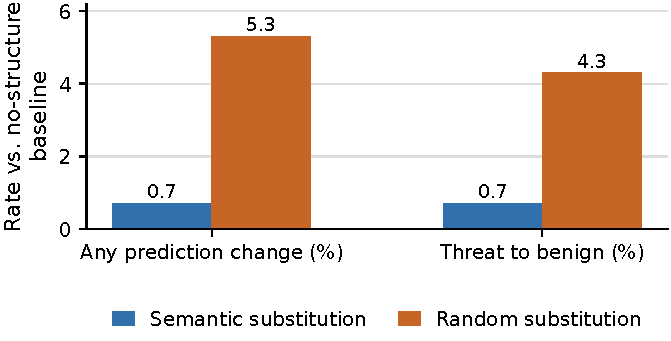
\includegraphics[width=0.8\textwidth]{img/semantic_no_structure.pdf}
  \caption[Direction of change under forced semantic reliance]{Predictions
  changed relative to the no-structure baseline on the test split, overall and
  in the threat-to-benign direction.}
  \label{fig:semantic_sub_no_structure}
\end{figure}

Figure~\ref{fig:semantic_sub_no_structure} adds a directional detail the
counts do not show. Of the 5.3\% of predictions that random substitution
changes, 4.3 percentage points are threats drifting to the benign side and
none move the other way, so the damage done by destroying meaning falls
entirely in the dangerous direction. The synonym regime changes two
predictions in all, both in that same direction but too few to weigh against
thirteen.

Together the two experiments prove the two claims stated at the outset of
the section, and they do so only in combination. The first showed that the
deployed framework does not depend on exact semantic identities, but could
not distinguish robustness from disregard; the second showed that the
stability is not disregard, because once the compensation is removed the
branch responds precisely to the destruction of meaning, though no deployed
configuration operates without structure. Read together they answer RQ1: the
semantic representations generalise at the level of meaning, and
understanding at that level is precisely the property expected to transfer
to operations and threats not seen during training, an expectation the
generalisation study of Section~\ref{sec:generalisation_results} tests
directly.

Throughout this section the model was held fixed while the semantic content
of its input was varied. The next section inverts the design: the data and
its perturbation tracks are held fixed while the detector varies. The
lexical, ordering, and combined tracks of
Section~\ref{subsec:robustness_eval} are aimed at the four single-paradigm
baseline families, detectors that possess only one of the framework's three
views, and the comparison establishes what the redundancy documented across
the last three sections is worth when it is absent.


\section{Baseline Comparison Against Single-Paradigm Baselines}
\label{sec:baseline_comparison}
% Objective: test whether jointly modelling the three dimensions beats
% single-paradigm detectors (RQ3). Identical splits. Carries the
% paradigm-targeting attack tracks of subsec:robustness_eval
% (lexical/ordering/combined + structure attack). TGNN reference numbers
% under those attacks (robustness_compare_dual: rename+dilution 2 missed /
% interleave 0 / combined 2 of 275; static_vs_existing_tgnn_strict:
% structure drop/rewire/inject 0 missed, recall 1.000).

A framework that fuses structural, semantic and temporal evidence is only worth
its added complexity if no single one of those views, developed to its full
strength, can match it. The ablations of the previous section answered that
question from within, by disabling the model's own components; this section
answers it from the outside, by setting the complete framework against four
established detectors, each of which commits to exactly one of the three views.
Classical machine learning over token counts stands for the raw identity of the
calls that appear, a static graph network for relational structure, a
semantic-embedding classifier for meaning, and a recurrent sequence model for
execution order. Each is a competent, fully trained detector in its own right
rather than a weakened strawman, and together they allow the margin between the
framework and any one paradigm to be attributed to the reasoning that paradigm
leaves out, which is the attribution question posed by RQ3.

All four competitors are trained and scored under the identical-split protocol
used throughout this chapter, on the same held-out traces as the framework, so
that every comparison rests on matched data. Performance is read through
threat recall and the count of threats missed, the operational quantities for
a detector whose task is to let no threat pass, alongside macro-F1 as a
balanced summary across the benign and threat classes. Read this way the
results pull in opposite directions: the baselines are genuinely competitive
on unaltered traces, and the separation appears only once those traces are
altered without changing what the malware does.

The two parts of the section follow that division. The first establishes the
clean comparison, placing all four competitors and the framework side by side on
unaltered traces to confirm that the contest begins from credible detectors
rather than convenient ones. The second then subjects each competitor to a
behaviour-preserving attack aimed squarely at its single dimension, renaming
calls against the identity- and meaning-based detectors, perturbing the graph
against the structural model, and reordering calls against the sequence model,
and reports where each gives way against a framework that misses no threat under
any of them. The clean comparison is taken up first.

\subsection{Cross-Paradigm Detection on Clean Traces}
\label{subsec:cross_paradigm}

Detection on unperturbed traces sets the floor for every later claim: a
framework unable to match its single-paradigm rivals before any manipulation
would have no robustness advantage worth defending. The clean comparison
therefore measures the framework and the four baselines on held-out traces
exactly as recorded, with no attack applied, and asks the narrow question of
whether the framework is even competitive at the starting line. It is
competitive but holds no clear lead. The strongest baselines match its perfect
threat recall and several exceed it on aggregate macro-F1, so unperturbed
detection alone does not justify the added complexity; what this section can
establish for the framework turns on what happens once the traces are
perturbed.

The comparison runs across two evaluation groups, each scored on the set its own
baselines were run against, so every model meets the framework on identical
traces. The classical and structural baselines use $475$ traces from the held-out
validation and test splits plus further withheld malicious samples; the semantic
and sequential baselines use the $325$ held-out validation and test traces. The
framework runs on both and so appears in each group of
Table~\ref{tab:baseline_clean}, whose class proportions differ from the test
split, so these macro-F1 values are not comparable with
Section~\ref{sec:main_results}.

\begin{table}[H]
\centering
\small
\begin{tabular}{@{}lcccc@{}}
\toprule
\textbf{Model} & \textbf{Threat recall} & \textbf{Threats missed} & \textbf{Macro-F1} & \textbf{Accuracy} \\
\midrule
\multicolumn{5}{@{}l}{\textit{Evaluation set A: 475 traces (200 benign / 200 other-malware / 75 ransomware)}} \\
\midrule
Classical: Random Forest & $100.0\%$ & $0 / 275$   & $0.847$ & $0.905$ \\
Classical: XGBoost       & $100.0\%$ & $0 / 275$   & $0.874$ & $0.920$ \\
Static GNN: GCN          & $100.0\%$ & $0 / 275$   & $0.604$ & $0.827$ \\
Static GNN: GAT          & $100.0\%$ & $0 / 275$   & $0.800$ & $0.884$ \\
Proposed framework       & $100.0\%$ & $0 / 275$   & $0.827$ & $0.895$ \\
\midrule
\multicolumn{5}{@{}l}{\textit{Evaluation set B: 325 traces (200 benign / 50 other-malware / 75 ransomware)}} \\
\midrule
Semantic-embedding MLP   & $97.6\%$  & $3 / 125$   & $0.769$ & $0.849$ \\
Sequential BiLSTM        & $96.8\%$  & $4 / 125$   & $0.840$ & $0.892$ \\
Proposed framework       & $100.0\%$ & $0 / 125$   & $0.763$ & $0.855$ \\
\bottomrule
\end{tabular}
\caption{Detection on clean, unperturbed traces.}
\label{tab:baseline_clean}
\end{table}

Threat recall and the count of missed threats give the operational reading, the
quantities by which a deployed detector is judged, while macro-F1 and accuracy
describe the finer three-class behaviour beneath the binary decision. The macro-F1
credited to the framework falls from the larger group to the smaller because the
smaller set carries far fewer other-malware traces, which sharpens the
ransomware-versus-other-malware confusion that a macro average penalises; the
shift reflects the composition of the evaluation set, not a change in the model.

On the larger group every model recovers every threat, so the comparison rests
entirely on the macro-F1 column, and there the classical detectors are the
strongest performers: the boosted ensemble attains the highest aggregate score
in this group, above the framework's own. Token-frequency features thus suffice
while the recorded call names remain intact, which is exactly what should be
expected of clean data. The structural baselines are more uneven, the
attention-based graph network competitive while the convolutional variant
trails the field by a wide margin on three-class discrimination. The framework
settles in the middle of the range.

On the smaller group the aggregate ordering turns against the framework while the
operational ordering turns in its favour. The sequential model records the highest
macro-F1 of the three and the semantic model edges the framework as well, yet both
purchase that advantage by letting threats through, four undetected for the
sequential model and three for the semantic, where the framework lets none escape.
The direction of these margins matters more than their size: in both cases a
cleaner aggregate score was bought with missed threats.

The clean comparison assumes that the recorded trace mirrors what the program
did. Whether the framework earns its complexity therefore depends on what
happens when that assumption fails, which is where the comparison turns next.

\subsection{Robustness Under Behaviour-Preserving Attacks}
\label{subsec:baseline_failure_modes}

Robustness, not accuracy on pristine input, is what an adversary ultimately
contests, and it is the property on which the clean comparison stayed silent.
Modelling three views rather than one should earn nothing on traces that every
paradigm already reads correctly, and everything on traces that have been altered
so that a single view no longer suffices. An adversary who expects the trace to be
inspected will change the trace, not the behaviour behind it. Altered traces are
therefore the normal setting for detection rather than a corner case, and this
part carries the comparison into it. Each baseline is subjected to a
behaviour-preserving manipulation aimed at the one dimension it depends upon, and
its response is placed beside the framework under
the identical manipulation, so that the cost of relying on a single view can be
read directly against the benefit of fusing three.

These manipulations are not abstract stress tests but the everyday repertoire of malware
evasion, which is why a detector's standing under them matters more than its
standing on pristine traces. Authors routinely rename or wrap API calls whenever
they recompile or repack a sample, so that a behaviourally identical program
presents an unfamiliar vocabulary; the meaning-preserving rename reproduces this,
substituting synonymous or trivially altered names for the calls actually issued.
A more deliberate variant disguises a call as an unrelated but legitimate
operation, the mimicry tactic by which malicious activity is dressed in
benign-looking names, and the out-of-context rename reproduces it by drawing
replacements from a pool of real but behaviourally unrelated Windows APIs.
Reordering mirrors the reshuffling of recorded calls, a rewrite that leaves the
executed behaviour intact while defeating any signature keyed to a fixed call
order; it is applied here as a complete permutation, so the result is a worst
case. Padding the trace with benign activity
reproduces junk-call and dead-code insertion, the familiar dilution of malicious
density beneath a mass of innocuous behaviour. For the structural baseline the
corresponding move operates on the graph itself, dropping and rewiring edges and
injecting decoy nodes, as an incompletely observed or deliberately noised
execution would appear. Every one of these leaves the malware's actual behaviour
unchanged, which is exactly what makes them fair: a model that reasons about
behaviour should have little reason to be fooled, and each attack is matched to the
paradigm whose single view it most directly undermines.

These results need more than threat recall, because the baselines fail in
opposite directions. A detector can fail by missing threats, predicting
benign for traces it can no longer recognise, or by crying wolf, flagging
everything as a threat once its input dissolves into noise. The first inflates the
count of missed threats; the second drives it to zero for the wrong reason,
flooding the benign class with false alarms instead. The second failure is
invisible to threat recall. The outcomes are therefore read through missed threats
and false positives together, with macro-F1 as the single figure that both
directions depress, and are collected in Table~\ref{tab:baseline_robustness}.

\begin{table}[H]
\centering
\small
\begin{tabular}{@{}lccc@{}}
\toprule
\textbf{Model} & \textbf{Threats missed} & \textbf{False positives} & \textbf{Macro-F1} \\
\midrule
\multicolumn{4}{@{}l}{\textit{Classical, API rename (475 traces; clean macro-F1 $0.874$)}} \\
\quad XGBoost   & $275 / 275$ & $0 / 200$ & $0.198$ \\
\quad Framework & $2 / 275$   & $7 / 200$ & $0.812$ \\
\midrule
\multicolumn{4}{@{}l}{\textit{Static GNN, graph perturbation (475 traces; clean macro-F1 $0.800$)}} \\
\quad GAT       & $144 / 275$ & $2 / 200$ & $0.404$ \\
\quad Framework & $0 / 275$   & $7 / 200$ & $0.823$ \\
\midrule
\multicolumn{4}{@{}l}{\textit{Semantic, API rename (325 traces; clean macro-F1 $0.769$)}} \\
\quad Semantic MLP, meaning-preserving & $8 / 125$   & $6 / 200$ & $0.499$ \\
\quad Semantic MLP, out-of-context     & $125 / 125$ & $0 / 200$ & $0.254$ \\
\quad Framework, out-of-context        & $0 / 125$   & $7 / 200$ & $0.744$ \\
\midrule
\multicolumn{4}{@{}l}{\textit{Sequential, reorder and rename (325 traces; clean macro-F1 $0.840$)}} \\
\quad BiLSTM, reordered    & $5 / 125$  & $10 / 200$   & $0.728$ \\
\quad BiLSTM, renamed      & $0 / 125$  & $200 / 200$  & $0.136$ \\
\quad Framework, reordered & $0 / 125$  & $6 / 200$    & $0.758$ \\
\quad Framework, renamed   & $0 / 125$  & $7 / 200$    & $0.744$ \\
\bottomrule
\end{tabular}
\caption{Robustness under behaviour-preserving attacks.}
\label{tab:baseline_robustness}
\end{table}

The classical detector illustrates the missing-threat failure in its starkest
form. On clean traces the boosted ensemble is the strongest model in the study,
yet renaming the API calls, while padding the trace so its length is unremarkable,
erases every feature the term-frequency representation was built on: not one of
the 275 threats is caught, and the model labels the entire malicious population
benign. Its macro-F1 falls from the best in the comparison to below a fifth. The
bagged ensemble fails in exactly the same way and to the same figures, so the
collapse belongs to the paradigm rather than to one model's tuning. The
framework, reading the same renamed traces, misses two threats and holds its
aggregate score almost unchanged, because the renamed calls still occupy the same
structural positions and the same execution order that its other two views encode.

The structural baseline fails on the axis it alone represents. Dropping and
rewiring a third of the graph's edges and injecting spurious nodes, all while
preserving the recorded API activity, drives the attention-based network from
competitive to broken: it misses 144 of the 275 threats, more than half, as the
topology it classifies on is dismantled beneath it. The framework absorbs the
identical structural damage without missing a single threat, its semantic and
temporal views supplying the evidence the corrupted graph no longer carries.

The semantic baseline draws out a subtler distinction, between meaning that can be
recovered and meaning that has been destroyed. A meaning-preserving rename, which
substitutes synonymous or lightly suffixed names, degrades it sharply on
discrimination, its macro-F1 halving, yet its threat recall largely survives
because the pretrained encoder maps the altered names close to the originals and
only a handful more threats slip through. Replacing each call instead with an
unrelated but genuine Windows API, a name that is plausible rather than unknown,
removes that lifeline entirely: the encoder embeds a real but wrong behaviour, and
the model misses all 125 threats, judging every manipulated trace benign. The
framework, exposed to the same out-of-context substitution, misses none,
because a change of names leaves its structural and temporal views untouched,
and Section~\ref{sec:ablation_results} showed those two recover every threat
on their own.

The sequential model is the one baseline that withstands the attack aimed at its own
dimension. Shuffling the call order degrades it only gracefully, from a clean
macro-F1 of $0.840$ to $0.728$ with five threats missed, evidence that it reads a
real ordering signal rather than a fixed template. Its fragility lies elsewhere. A
rename sends almost every token outside the self-contained vocabulary it learned,
and an ordered model over an all-unknown sequence has no signal left to weigh; it
collapses not by missing threats but by crying wolf, flagging all 200 benign traces
and posting a macro-F1 of $0.136$. Read naively, the model misses no threat under
this rename; yet that zero is an artefact of surrender rather than skill, since a
detector that flags everything catches every threat trivially while distinguishing
nothing. It is a failure and not a success, meaningful only beside the two hundred
false alarms that expose it as such. The sequence model therefore leans more on
which calls appear than on the order it was built to exploit: it survives reordering
but not renaming. The framework misses no threat under either manipulation, flagging
six benign traces under the reordering and seven under the rename, because it never
stakes its decision on a closed vocabulary: its semantic branch re-encodes each
unfamiliar name by meaning rather than discarding it as unknown.

\begin{figure}[t]
\centering
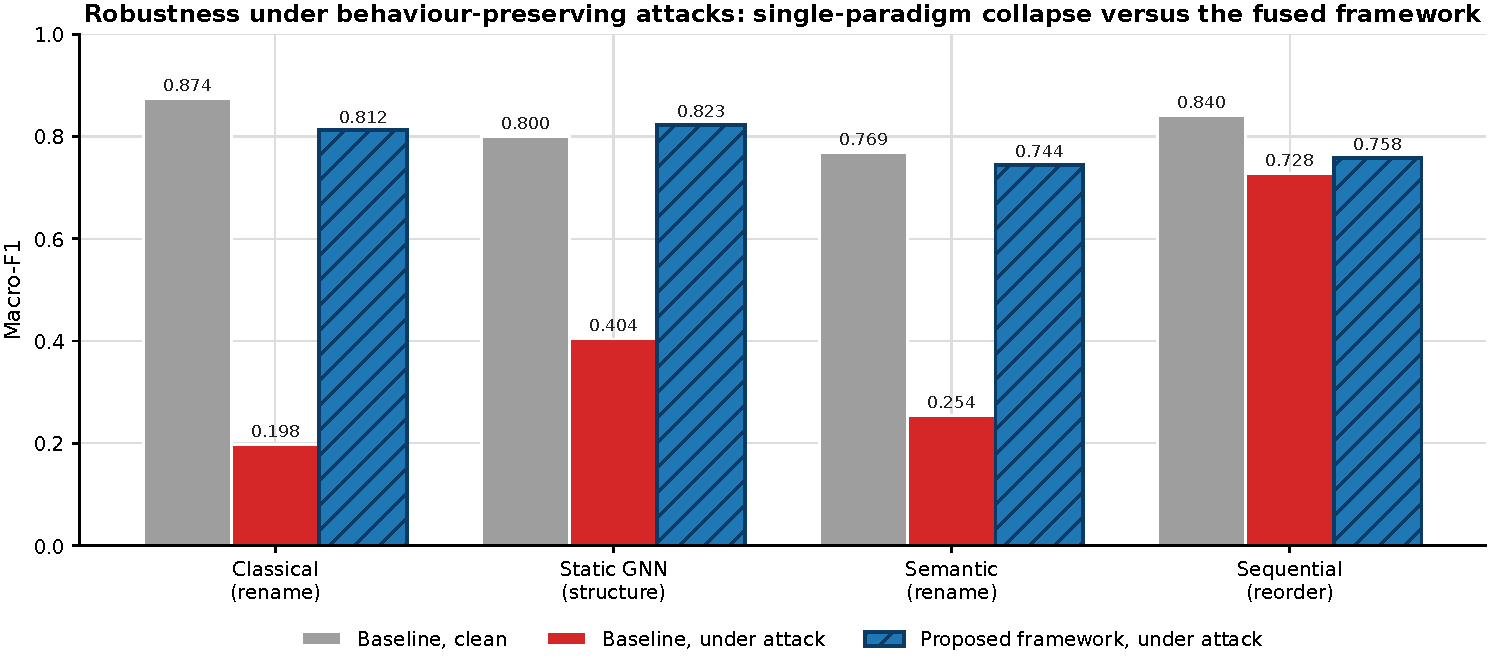
\includegraphics[width=\textwidth]{img/baseline_robustness_comparison.pdf}
\caption[Macro-F1 under behaviour-preserving attacks]{Macro-F1 of each baseline on
clean traces (grey), under the attack aimed at its dimension (red), and of the
proposed framework under the identical attack (blue, hatched). Three baselines
collapse on their axis and the sequence model degrades under reordering, while the
framework holds throughout.}
\label{fig:baseline_robustness}
\end{figure}

Figure~\ref{fig:baseline_robustness} draws the four confrontations together. The
pattern is uniform in its consequence if not in its mechanism: three of the four
baselines collapse towards the floor, the fourth, the sequence model under
reordering, dips but survives, and in every case the framework holds level with its
clean score. The single view each baseline embodies is load-bearing,
and knocking it out brings the detector down; the framework, resting on three,
never loses more than a few points of aggregate score and never surrenders the
threat line.

These confrontations answer RQ3, the question the section set out to settle. Jointly
modelling relational, semantic and temporal evidence is not a clean-data
refinement, since on clean data it changed nothing, but a robustness property:
every single-paradigm detector examined, each a competent representative of an
established practice, is broken by a behaviour-preserving manipulation that a real
adversary can apply for free, three of them on the very dimension they rely
upon. The framework meets all four attacks with at most two missed threats and an
aggregate score that barely moves. Because each baseline stands in for one of the
framework's own branches, this external result corroborates the internal ablation
of the previous section from the opposite direction: no single view is sufficient,
and the detector's resilience is a property of their fusion rather than of any one
of them. Against an adversary who manipulates how behaviour is recorded, the
proposed framework does not merely match the single-paradigm alternatives; it is
the only one of the five that continues to work. What remains untested is the other
face of the operational problem, not an adversary reshaping a known threat but a
threat the model has never seen at all, and it is to that question of
generalisation that the evaluation turns next.


\section{Generalising to an Unseen Threat Source}
\label{sec:generalisation_results}
% Objective: measure generalisation to threats unseen during training
% (RQ5, and RQ1 for semantic generalisation).

A detector earns its place in deployment only if it still works on threats that
did not exist, or had not been collected, when it was trained. Malware is produced
continuously and from countless sources, so a model that recognises only the
specific behaviours present in its training set is obsolete the moment the threat
landscape moves. The robustness established in the previous section concerned a
known threat disguised by an adversary; the demand here is the complementary one of
a threat the framework has never encountered at all, drawn from an independent
source with its own API vocabulary and behavioural profile. This section asks
whether the framework's behavioural reasoning transfers to such out-of-distribution
threats rather than only to rearrangements of familiar ones, which is the
generalisation question posed by RQ5.

Answering it takes two steps in order. The claim that these threats are genuinely
unseen has to be earned rather than asserted, so the evaluation samples are first
shown to come from a separate source with no sample overlap with training and
an API-usage profile that diverges sharply from it: calls that dominate the
training behaviour all but disappear, and calls absent from training appear in
force. With that distributional gap established, the framework is then evaluated on
the unseen threats directly, and the finding is that the change of surface
vocabulary, which would defeat a detector that had learned particular tokens, costs
the framework nothing, since it misses none of them. Because the previous section
already set the framework against competing paradigms, the evaluation here reports
the framework on its own; the question is one of transfer, not comparison.

The framework generalises because it classifies behaviour, how calls are wired
and sequenced and what they mean, rather than the particular names a given
family happens to use, so that a wholesale change of vocabulary leaves the
behavioural signal it relies on intact. The profile of the unseen distribution
is taken up first, since it sets the bar the framework must then clear.

\subsection{Profiling an Unseen Threat Distribution}
\label{subsec:lofo_results}

A detection result on unseen threats is only as convincing as the claim that the
threats were unseen to begin with. Were the evaluation samples to resemble the
training data in their behaviour, catching them would demonstrate familiarity
rather than generalisation, and the outcome would prove little about transfer. The
profile is therefore established before any detection is measured.

The departure is measured on the behavioural vocabulary itself, the API calls that
constitute each trace. The distribution of calls across the training corpus is
compared against their distribution across the unseen set, a body of $110$ threat
traces held apart from training, in each case as the fraction of total calls that
each API accounts for, so that a difference reflects a genuine change in behaviour
rather than a difference in the number of samples.
Three quantities summarise the gap, reported in Table~\ref{tab:unseen_shift}: how
many calls occur in the unseen set that the model never saw in training, how far
the two distributions stand apart as a whole, and how much of their most frequent
behaviour they share.

\begin{table}[H]
\centering
\small
\begin{tabular}{@{}lr@{}}
\toprule
\textbf{Measure} & \textbf{Value} \\
\midrule
Unseen threat samples (from a separate source) & $110$ \\
Samples overlapping the training corpus & none \\
Distinct API calls (training vs unseen) & $323$ vs $255$ \\
Unseen calls absent from training & $71$ ($27.8\%$ of vocabulary) \\
Jensen--Shannon divergence ($0$--$1$) & $0.534$ \\
Shared calls among the twenty most frequent & $6$ of $20$ \\
\bottomrule
\end{tabular}
\caption[API distribution shift, training versus unseen]{The unseen evaluation set against the training corpus, measured on the
distribution of API calls. The divergence and overlap figures treat each set as a
distribution over calls and are therefore independent of the number of samples in
each.}
\label{tab:unseen_shift}
\end{table}

The two behavioural vocabularies are substantially different. Of the $255$ distinct
calls in the unseen set, $71$ never appear in training at all, and although these
are individually infrequent they still account for roughly a ninth of the unseen
call volume, a body of behaviour with no training precedent whatever. The
distributions as a whole stand far apart: their Jensen--Shannon divergence, a
bounded measure on which zero denotes identical distributions and one denotes no
shared mass, reaches $0.534$, and of the twenty calls that occur most often only
six are common to both sets. The samples are moreover taken from a separate
source with no overlap with the training corpus, so the divergence cannot be a
resampling of the same threats.

\begin{figure}[H]
\centering
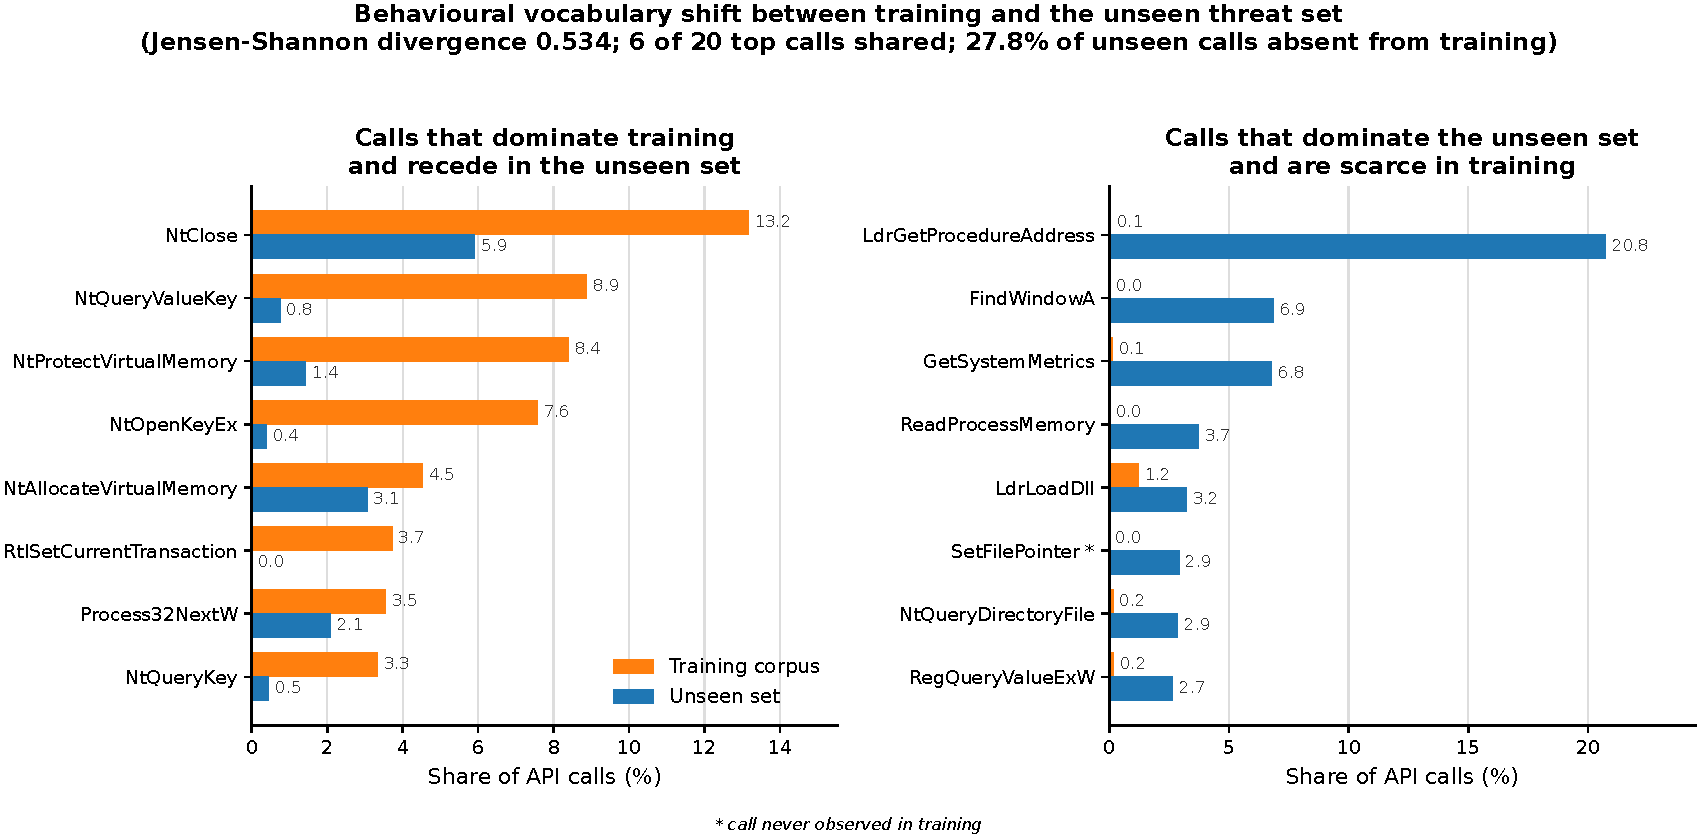
\includegraphics[width=0.90\textwidth]{img/unseen_distribution_shift.pdf}
\caption[Behavioural vocabulary shift, training versus unseen]{Share of API calls in training and in the unseen set. Left: calls dominating training. Right: calls dominating the unseen set.}
\label{fig:unseen_shift}
\end{figure}

Figure~\ref{fig:unseen_shift} shows where the shift falls, and what each profile
means in behavioural terms. The calls that dominate the training corpus are the
signatures of in-memory tampering and registry inspection: NtProtectVirtualMemory,
which alters the access protection of a memory region and is the tell-tale of code
injection and unpacking; NtQueryValueKey and NtOpenKeyEx, which read and open
registry keys as a sample inspects the system's configuration; and NtClose, the
ubiquitous closing of a handle. Each of these recedes sharply in the unseen set,
several to a fraction of a percent. The calls that dominate the unseen set describe
a different activity altogether. LdrGetProcedureAddress, which looks up the address
of a function inside an already-loaded library at run time so that a program can
call it without declaring it in advance, alone accounts for a fifth of the unseen
calls yet is all but absent from training; it is the classic means by which packed
and loader malware conceal which routines they use. Around it sit FindWindowA and
GetSystemMetrics, which query the windowing environment and display configuration,
and ReadProcessMemory, which reads the memory of another running process,
behaviours characteristic of loaders and reconnaissance rather than the
injection-heavy profile the model learned. The unseen threats are not louder or
quieter renderings of the training malware; they exercise a different behavioural
repertoire.

The evaluation set is therefore genuinely out of distribution on the dimension that
matters most to a behavioural detector, the calls a program makes. It presents the
model with calls it never encountered in training and, alongside them, a new
behavioural context: calls that sat at the margins of the training data now dominate
the trace, so that even familiar behaviour arrives in an unfamiliar proportion. A
detector that had learned the specific vocabulary of its training threats would be
defeated twice over: the calls it relies on are largely gone, and the calls that
remain are ones it hardly saw. Whether the framework nonetheless recognises these
threats, and if so on what evidence, is the question the profile has now made
precise, and it is settled next.

\subsection{Detection Performance on Unseen Threats}
\label{subsec:zeroday_results}

The profile just drawn sets a demanding test, and the framework meets it without
exception. Evaluated on the $110$ unseen traces, the model classifies every one as
a threat: no unseen sample is labelled benign, and threat recall on the unseen set
is complete. The evaluation places these threats alongside the held-out benign and
seen-threat traces of the standard test protocol, so that performance on the
unfamiliar samples can be read against performance on familiar ones, and it asks
two things of the result. The first is whether the unseen threats are caught at
all, measured through threats missed and threat recall; the second is whether they
are caught with conviction or merely scraped over the decision boundary, measured
through the probability the model assigns to the threat outcome.
Table~\ref{tab:zeroday_detection} reports the former and
Figure~\ref{fig:zeroday_conf} the latter.

\begin{table}[H]
\centering
\small
\begin{tabular}{@{}lccc@{}}
\toprule
\textbf{Threat group} & \textbf{Samples} & \textbf{Threats missed} & \textbf{Threat recall} \\
\midrule
Unseen threats & $110$ & $0$ & $100\%$ \\
Seen threats (test and validation) & $130$ & $0$ & $100\%$ \\
\bottomrule
\end{tabular}
\caption[Detection on unseen versus seen threats]{Threat detection on the unseen set against the seen threats of the
standard test protocol, for the reported framework. Benign specificity on the same
evaluation is $97\%$: six false positives among two hundred benign traces.}
\label{tab:zeroday_detection}
\end{table}

Not one of the $110$ unseen threats is missed, a threat recall that matches the
model's recall on the seen threats of the test and validation splits exactly. The
parity is the substance of the result: exposure to an unfamiliar source and a
rebalanced vocabulary produces no measurable loss of recall relative to samples of
the kind the model was trained on. The detection is moreover not bought by
indiscriminate suspicion, since on the same evaluation the model keeps a benign
specificity of $97\%$, flagging only six of two hundred benign traces; the unseen
threats are separated from clean software rather than swept up with it.

\begin{figure}[H]
\centering
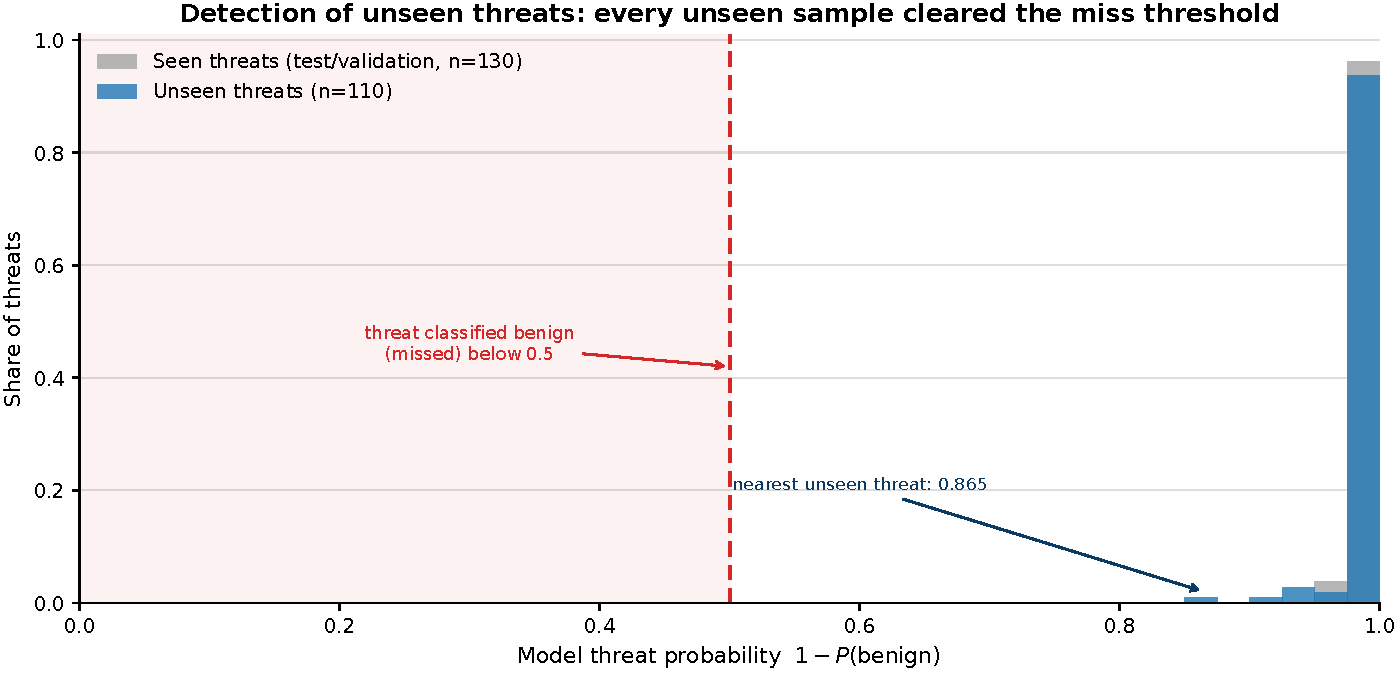
\includegraphics[width=\textwidth]{img/zeroday_detection_confidence.pdf}
\caption[Detection confidence on unseen threats]{Threat probability the model
assigns to each threat, for the unseen set and for the seen threats of the test and
validation splits. The dashed line marks the $0.5$ boundary below which a threat
would be classified benign; the shaded region to its left, where a miss would
occur, contains no sample of either kind.}
\label{fig:zeroday_conf}
\end{figure}

Figure~\ref{fig:zeroday_conf} shows that the unseen threats are caught with margin
rather than by a whisker. The probability assigned to the threat outcome sits close
to one for almost every unseen sample, with a median of $0.99$, and the least
confident of the $110$, at $0.865$, still stands far to the right of the decision
boundary. No unseen sample, and no seen threat, falls into the region where a miss
would occur. The unseen distribution sits only marginally lower than the seen one,
so the unfamiliarity established earlier costs the model a little confidence but
never a detection.

The reason this holds is visible in how the decision is reached. Averaged over the
$110$ unseen threats, the decision is driven by the structural view, at a mean
weight of $0.41$, though not by it alone: the temporal and semantic views still
carry shares of $0.33$ and $0.25$. It is this blend that yields the smooth and
confident probabilities of Figure~\ref{fig:zeroday_conf}, the structural view
supplying the backbone of the judgement while the temporal and semantic views
steady and sharpen it. What changes relative to the model's average behaviour is
the balance rather than the participation: across the full evaluation the semantic
view carries about as much weight as the structural one, whereas on the unseen
threats the gate shifts a portion of its trust towards the structure and timing of
the behaviour. The shift is a reweighting and not an abandonment. The semantic
view still carries a quarter of the decision, and
Section~\ref{sec:robustness_results} established that it reads what a call does
rather than which name it bears, so an unfamiliar name arrives as behaviour rather
than as an unknown token. The framework generalises because a change of vocabulary
leaves all three views something to read.

This settles RQ5, the generalisation question the section posed. Confronted with threats
from an independent source, carrying calls it had never seen and a behavioural
profile rebalanced away from its training experience, the framework detected every
one, with confidence comparable to the threats it already knew and without
sacrificing its discrimination of benign software. It achieves this not by having
memorised the vocabulary of past malware, which the profiling showed would have
left it stranded, but by reading behaviour through all three of its views: an
unfamiliar name still carries meaning, and the structure and timing around it are
unchanged. Detection under adversarial manipulation and
detection of an unseen source have now both been accounted for; what remains,
asserted here in the gate's reallocation of trust but not yet examined in its own
right, is the framework's capacity to explain which behaviour drove a given
decision, and it is to that capacity the evaluation turns next.


\section{Interpretability and Decision Attribution}
\label{sec:interpretability_results}
% Objective: demonstrate that the framework can explain its predictions (RQ4):
% which behavioural dimension and which API subgraph drove each threat/benign
% decision. Source: scripts/explain_rq4_behavioral_decisions.py and
% results/rq4_explanations/.

The evaluation so far has measured what the framework decides and how reliably it
does so; it has not yet asked whether those decisions can be understood. For a tool
meant to support human analysts that question is not secondary. An alert that
cannot say why it fired is difficult to trust and harder to act upon, and a model
whose reasoning stays hidden cannot be held to the claim, central to this thesis,
that it detects threats by their behaviour rather than by surface cues. This
section therefore turns from whether the framework is right to whether it can show
why, which is the interpretability question posed by RQ4.

An explanation of a decision has two parts: which kind of evidence weighed most,
and what that evidence actually was. The first is already in hand. The adaptive
gate that fuses the three views records, for every prediction, how much each view
contributed, and the branch-contribution analysis of
Section~\ref{sec:component_attribution} read those weights as a faithful,
per-decision attribution of the behavioural dimension behind a verdict, structural,
semantic or temporal. Because the weights are the very quantities the model uses to
combine its branches, that attribution is exact rather than an after-the-fact
approximation of the sort a separate explainer would supply. Knowing that a
decision rested on structure or on timing, however, is only half of an explanation;
it does not say which structures or which behaviours. This section supplies the
other half.

The framework can supply it because it decides over an explicit graph of behaviour
rather than an opaque feature vector, so a prediction can be traced back to the
concrete activity that produced it. From a threat verdict the calls that most
influenced the outcome can be recovered, together with the region of the call graph
they occupy, the order in which they executed, and any file, registry, process and
network objects they touched, and read back as a legible account of why the sample
was flagged. What follows demonstrates this reconstruction on a single decision and
puts to it the question that matters for interpretability: whether the behaviour it
surfaces is recognisably malicious rather than incidental.

\subsection{Explaining a Decision Through Behaviour}
\label{subsec:worked_explanations}

To make the reconstruction concrete, consider one threat decision in full. The
sample is a malware executable from the held-out test split; the framework
classifies it as a threat and assigns its malware family a probability of $0.95$,
and every element of the explanation is a quantity the model itself computed in
reaching that verdict, with no external labelling of which calls are suspicious. The
account rests on three ingredients, each read from the trained model. The salience
of each API call is measured by combining the gradient of the predicted-class score
with respect to that call's feature vector with the vector itself, so the calls that
most influenced that score are identified directly rather than guessed at. Each
salient call is then placed back in the graph, alongside the calls that precede and
follow it in execution order, the relations that connect it, and any process, file,
registry and network nodes in its neighbourhood. The branch weights, finally, record
which of the three views the decision leaned on. Together these turn a single
probability into a behavioural narrative. Figure~\ref{fig:decision_explanation}
draws that narrative for the sample at hand.

\begin{figure}[H]
\centering
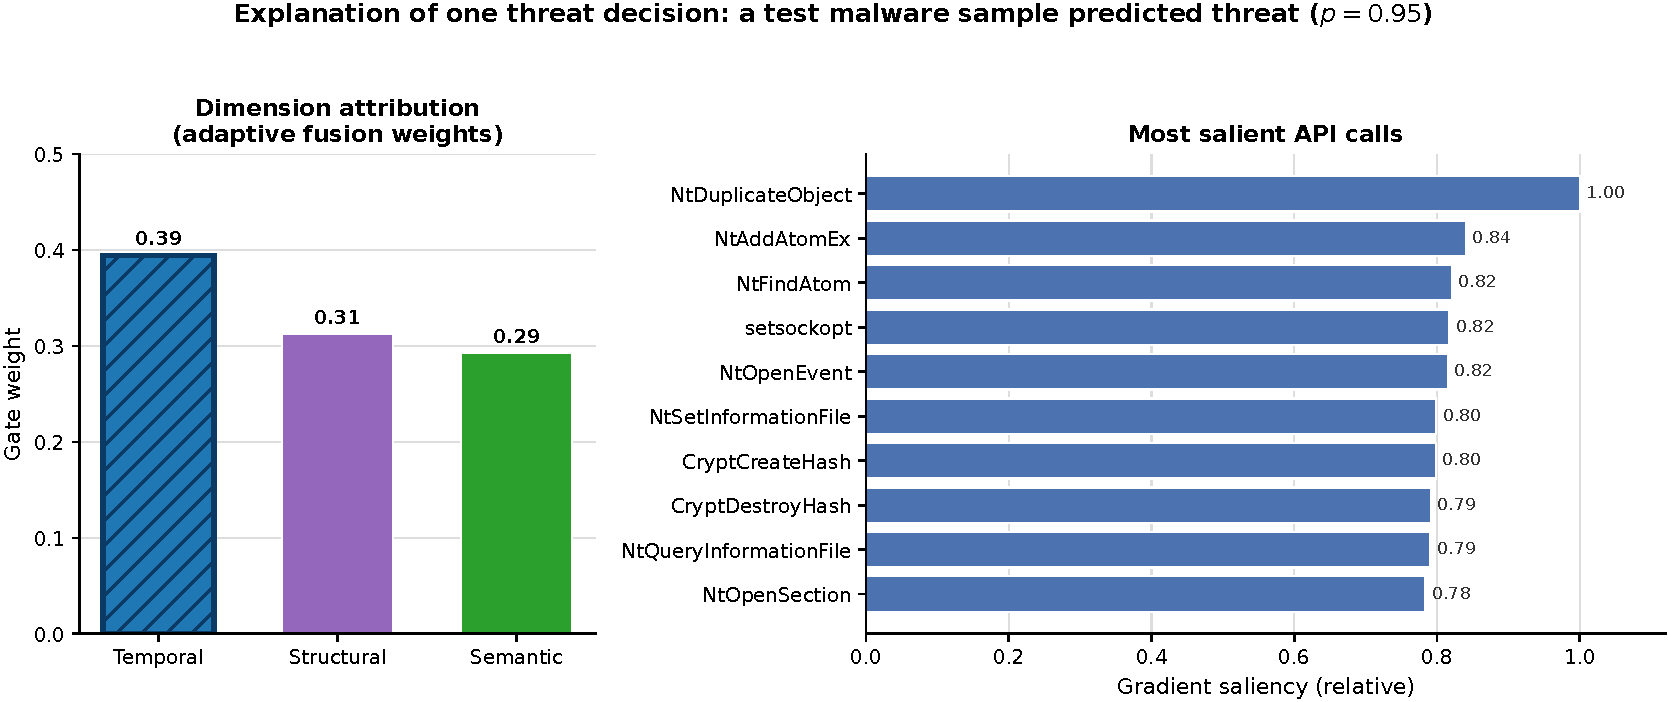
\includegraphics[width=\textwidth]{img/decision_explanation.pdf}
\caption[Explanation of one threat decision]{The framework's own explanation of
a single threat decision.}
\label{fig:decision_explanation}
\end{figure}

The decision leaned most on the temporal view, at a gate weight of $0.39$ against
$0.31$ for the structural and $0.29$ for the semantic, so the order of behaviour
carried the strongest signal, though all three views contributed materially. The
most salient calls span several distinct capabilities rather than one repeated
action: handle duplication through NtDuplicateObject, which drew the maximum
saliency, atom-table manipulation through NtAddAtomEx and NtFindAtom, network-socket
configuration through setsockopt, event synchronisation through NtOpenEvent,
cryptographic hashing through CryptCreateHash and CryptDestroyHash, and
file-attribute changes through NtSetInformationFile. These calls are spread across
the whole recorded trace rather than clustered in one part of it, yet each sits in a
burst of immediate transitions, which is the temporal evidence behind the weight the
gate placed on that view. Every one of them is anchored to the same process, the
sample's own executable, and that anchoring is the one structural relation the
ablation of Section~\ref{subsec:relation_feature_ablation} found to be load-bearing.
The picture the model assembles is therefore not a lone tell-tale call but several
distinct capabilities, cryptographic, networking, synchronisation and file,
exercised in bursts by a single process, which is a recognisable profile of active
malware rather than of benign software.

What makes this an explanation rather than a plausible story is that each of its
elements is a quantity the model actually used. The salient calls are those whose
feature vectors weighed most on the predicted-class score, the relations are the
graph edges message passing traversed, and the branch weights are the coefficients
of the fusion. It remains an interpretability aid grounded in the model's own
computation rather than a formal causal proof, but because nothing in it is invented
after the fact, it is faithful to the decision in a way that a post-hoc
approximation trained to imitate the model would not be. An analyst reading the
report can see the specific behaviour behind an alert and the dimension along which
it was judged, and can corroborate or dispute it against the trace, which is
precisely the auditability a bare score denies.

Taken with the dimension-level attribution of
Section~\ref{sec:component_attribution}, this answers RQ4. A prediction of the
framework is not an opaque number but a decision that can be opened: the branch
weights say which kind of behaviour was decisive, and the saliency-and-graph
reconstruction says which concrete calls, in which order and touching which
resources, made the case. What makes the framework hard to evade is also what makes
it possible to read: the representation it reasons over is the representation it
reports. The evaluation is thereby complete: the framework detects threats
accurately, holds that accuracy under behaviour-preserving manipulation and against
threats from an unseen source, and can account for the behavioural grounds of each
decision it reaches. What those results amount to, and where their limits lie, is
the subject of the closing chapter.

\chapter{Conclusion, Limitations and Future Work}
\label{chap:future_work}

The preceding chapter established, experiment by experiment, what the proposed
framework does and how well it does it. This closing chapter steps back from the
individual results to ask what they amount to: what the work set out to solve, what
it has shown, where its boundaries lie, and what it opens up. It answers each
research question on the evidence of Chapter~\ref{chap:results}, states the
limitations that qualify those answers, and sets out the directions in which the
framework could be carried further.

\section{Conclusion}
\label{sec:conclusion}

Behavioural threat detection has long been caught between partial views of behaviour:
detectors that read only what a program calls, which obfuscation trivially defeats;
detectors that read only how those calls are arranged, which discard the meaning that
separates benign automation from malice; and detectors indifferent to when those
calls are issued, which lose the pacing that distinguishes rapid destruction from
ordinary work such as a scheduled backup. The problem this thesis set out to
solve was to detect threats from behaviour in a way that survived all three, by
reasoning
jointly over the three dimensions along which behaviour is expressed: the relations
between actions, the meaning of each action, and the order in which actions unfold.

\textbf{The novelty of the work.} The framework treats behaviour as one object
seen three ways: what a call means, the relations among the entities it touches,
and the order in which it was issued are reasoned over together within a single
schema-aware heterogeneous graph, not recovered from a view that discarded them.
Such a graph makes two demands of an aggregator at once, where the deciding edge is
often rare and its endpoints unseen in training, so attention is paired with a
GraphSAGE aggregator modified to consume edge features directly and which to trust
is learned per node and per feature. The gate that fuses the three branches works
the same way: one sample gives itself away by what it calls, another by how fast it
acts, so the model decides for each sample how much each of the three should
count.

Chapter~\ref{chap:results} put the framework to the test, and its experiments
support a definite conclusion on each of the five questions posed in
Section~\ref{sec:research_questions}. The evidence for each was set out there in
full, so what remains is to draw it together: to state what every question is now
answered to be, and how far that answer reaches.

\textbf{RQ1, semantic generalisation.} \emph{Can pretrained semantic embeddings
improve generalisation towards obfuscated or evolving behaviours unobserved during
training?} They can, and it takes the two experiments of
Section~\ref{sec:robustness_results} together to show it. Substituting every
semantic embedding while preserving what the call did left the framework's verdicts
unmoved, which alone settles nothing: a detector leaning on structure instead would
look exactly the same. Silencing the structural pathway removed that alternative.
Forced onto its semantic and temporal views, the framework then separated the two
regimes sharply, moving $0.7\%$ of predictions when each embedding was exchanged for
its nearest functional neighbour and $5.3\%$ when the content was destroyed
outright, $4.3$ of those percentage points being threats reclassified as benign.
Identity lookup cannot produce that gap, since neither regime leaves the original
vector in place for it to match. The semantic branch therefore reads the function of
an operation rather than its name, and that is the property which carries to
vocabulary the training data never contained. The claim is bounded to substitutions
that preserve behaviour by construction, and does not extend to an adversary willing
to change the behaviour itself.

\textbf{RQ2, complementarity of semantic, structural and temporal signals.} \emph{Do
the semantic, structural and temporal views carry complementary information, and
does modelling them together yield what none achieves alone?} They do, and the answer rests on two
measurements. The first, in Section~\ref{sec:component_attribution}, established that
the intact model genuinely draws on all three branches, with near-equal mean gate
weights and leadership that shifts by class, so no branch is decorative. The second,
in Section~\ref{sec:ablation_results}, established that the threat decision
nonetheless survives the loss of any one of them: on unperturbed traces the worst
single-branch removal still retained $95.8\%$ threat recall. The two reconcile because the views overlap on
the binary question: whether a sample is a threat can be recovered from any one of
them alone, imperfectly but well enough for detection to degrade gracefully rather
than fail, whereas naming its class correctly cannot, which is why only the full
model reaches the best exact-class accuracy in the study. Complementarity here therefore means two things at once: each branch adds
something of its own, and each can be covered by the other two. This holds for a
branch that is missing, not one under attack. The traces here were clean and the
remaining views untouched; the attacked case is taken up by RQ3 below.

\textbf{RQ3, end-to-end detection performance.} \emph{How does the framework compare
with representative detectors drawn from the established single-paradigm families
(baselines)?} On clean traces it holds no advantage over them, which is the expected
result: the framework was never meant to raise accuracy on unmanipulated data, but to
remove the single weakness an attacker can target.
Section~\ref{sec:baseline_comparison} set four competent detectors against it, one
committed to each single view, and the separation appears only once the traces are
manipulated. Three of the four then give way on the axis they were built around, and
the fourth on a different one. The framework lost at most two threats under any of
the four, and never more than two points of aggregate score. The reason is the
redundancy the ablation of Section~\ref{sec:ablation_results} measured, seen now from
outside: an attack on one dimension leaves the framework two intact views and a
single-view detector none.
The gain is therefore not accuracy but the absence of a load-bearing dimension, since
a gate that sets the balance sample by sample never lets one view carry enough of the
decision for its manipulation to overturn the verdict. The comparison is bounded to
the attacks tested, which are cheap and behaviour-preserving by design rather than
optimised against the model.

\textbf{RQ4, interpretability.} \emph{Can the framework attribute a decision to the
behaviour and the dimension that produced it?} It can, at two levels that answer
different analyst questions. The first, established in
Section~\ref{sec:component_attribution}, reads the fusion gate to name the
behavioural dimension that carried a verdict. In the worked example of
Section~\ref{sec:interpretability_results}, a sample classified as a threat with
$0.95$ of its probability on one malware family, the gate placed $0.39$ on the
temporal view, against $0.31$ for the structural and $0.29$ for the semantic. The
second descends to the behaviour itself, ranking the calls by their measured
influence on the decision and reading from the graph when each was issued and what
it operated on. For that sample these were several capabilities spanning
cryptography, networking, synchronisation and file access, all issued by one process
in tight bursts, in place of a single incriminating call. Both are composed entirely
of quantities the decision was made with, which is what separates them from an
explainer fitted to the model afterwards. What they deliver is an account faithful
to the computation rather than a proof of cause, and one an analyst can test against
the trace.

\textbf{RQ5, cross-source generalisation.} \emph{Does the framework generalise to
threats from outside its training experience?} It does, and
Section~\ref{sec:generalisation_results} measured the gap before testing across it.
The $110$ evaluation threats came from a separate source, withheld from training
entirely, more than a quarter of their distinct calls never appear in training, and
the operations they favour are ones the training malware barely touched. Every one
was returned as a threat, none of them close to the benign boundary, and six of the
two hundred familiar benign traces judged beside them were wrongly flagged. Why this
worked is what carries beyond the corpus. As the profiling had shown, nothing in the
call names could have supplied the recognition; the gate instead leaned harder on how
the calls were connected and when they occurred, while the semantic view kept a
quarter of the weight, still reading meaning out of names it had never met. That
reallocation is available only to a model that learns its own balance. The evidence
establishes transfer across one genuine shift of source and distribution, not breadth
across many threat families, which this corpus was not labelled to test.

The contribution of the work is therefore both architectural and empirical.
Architecturally, it is a single, end-to-end model in which structural, semantic
and temporal reasoning are learned together over one schema-aware heterogeneous
graph and fused by an adaptive gate that reweighs the three for every individual
decision. That gate is the architectural novelty: by letting the model itself decide
how each behaviour is judged rather than applying a fixed blend, it is what makes the
framework not only accurate but robust and self-explaining. Empirically, it demonstrates that behavioural
detection grounded in all three dimensions withstands the cheap, behaviour-preserving
evasions that defeat single-paradigm detectors, and that it does so without the
opacity such robustness usually costs. For practitioners this points towards a
detector whose alerts survive obfuscation, transfer to previously unseen malware, and
arrive with an account of the behaviour that triggered them, qualities that
current tools rarely offer together.

\section{Limitations}
\label{sec:limitations}

The strength of these findings is bounded by the conditions under which they were
obtained, and stating those bounds is part of reading the results honestly. The
most consequential is a matter of design. The framework constructs its
behavioural graph from a complete execution trace, delivered as a finished
sandbox report, and classifies that artefact, so it reaches a verdict after a
program has run rather than on the fly, while the program is still executing.
This suits the retrospective triage the evaluation targets. Detecting on the fly,
by growing the graph incrementally from events as they are emitted and revising
the decision as they arrive, would mean reconstructing and re-evaluating the
representation repeatedly as a trace unfolds; the computational resources and
time available to this work did not extend to that, so it is left as a direction
for further development rather than a bound the design cannot cross.

The temporal branch reads the call sequence with a bidirectional recurrent
network, whose effective memory horizon is finite, so on the longest traces
dependencies between distant events are unlikely to be carried in full. The
structural branch places every call two steps from every other through the process
that issued it, which bounds the effect rather than removing it.

The corpus is a snapshot, drawn from two sources at a fixed point in time, and
behaviour it does not contain cannot be learned from it; the ransomware class
in particular rests on relatively few samples, and its labels derive from VirusTotal
detections that vendors revise over time. The supplementary
collection supplies most benign training samples, so provenance was available
as a shortcut; the $110$ unseen threats of Chapter~\ref{chap:results} came from
that same sandbox and none was missed, so the grounding is not an artefact of how
either source was instrumented. That source contributed threats only, however, so the
benign side of the generalisation result was measured on familiar software rather
than on clean programs from the new source. Two sources are nonetheless few,
and every trace was produced on Windows, so wider validation and periodic
retraining are what a deployed setting would ask of it. Like any detector that
learns from observed execution, it also depends on there being behaviour to
observe: a sample that detects the analysis environment and withholds its
activity presents little to reason over.

Other choices were made for tractability rather than principle. Retaining a
high-dimensional semantic embedding for every call renders the largest
execution graphs expensive to store and to process, which shaped how much of
the corpus could be exercised at once. The adversarial evaluation, though
designed to cover the distinct axes an attacker can manipulate, tests a
representative rather than exhaustive set of transformations and does not
include an adaptive white-box adversary optimising directly against the model,
and no training run was repeated, so no reported figure carries an estimate of
run-to-run variance.

None of these bounds overturns the central findings. The robustness and
generalisation results hold on the sets against which they were measured, the
comparisons are fair within each experiment, and the interpretability is read from the
model's own quantities rather than from a stand-in. The attribution is bounded in a
way worth stating: a gate weight is the coefficient the fusion applies to a branch,
not a share of the decision, since the representations those weights scale differ in
magnitude. What the limitations qualify is the breadth of the claims rather than
their validity, and they mark the natural starting points for the work that should
follow.

\section{Future Work}
\label{sec:future_work}

Several of those boundaries suggest concrete next steps, and others follow from the
framework's modular design rather than from its limits. The framework at present
builds its behavioural graph offline, from a complete execution trace, and
classifies the finished artefact. The most consequential extension would move
detection online. A continuous-time dynamic graph formulation, in the manner of the
temporal graph networks set out in Section~\ref{sec:temporal_graph}, would let the
same behavioural engine ingest events as they are emitted and update its
representation incrementally, so that a verdict could be reached, and revised, while
a program is still executing rather than only after it has run to completion. Acting
before a program's behaviour completes is only possible on that basis, and the
graph-native design of the framework makes it a natural host for such a mechanism.

The temporal slot was left interchangeable by design, which invites
experimentation with the sequence model it houses. A
self-attention, transformer-based backbone is one candidate, offering direct
modelling of long-range dependencies between distant calls; the open question there
is operational cost, since attention scales quadratically with sequence length and
execution traces are long, so the value of such a backbone rests on making it cheap
enough to run at the volumes a deployed detector must handle. Reducing the per-call
representation and the resulting graph size, noted among the limitations, is part of
the same efficiency problem.

A complementary line is the selective state-space family of sequence models.
Their linear scaling in sequence length makes them
promising precisely where a transformer is costly. Developing a Mamba-based
temporal branch on the very long execution traces that most strain the current
model, and comparing it carefully against both the recurrent and the
attention-based alternatives on the same behavioural graphs, would settle which
sequence model the temporal slot should ultimately carry.

Beyond the engine itself, the clearest validation task is breadth. Exercising
the framework across additional sandboxes, platforms and threat sources would
test how far the behavioural grounding that served it here extends, and
calibrating its confidence under perturbation would let an operator weigh not
only what it decides but how surely. Two of the bounds above also invite direct work.
An adaptive adversary with access to the model, optimising a perturbation against the
gate rather than applying a fixed transformation, is the sterner test the attack
repertoire used here does not deliver, and repeating the training across seeds would
put an interval around every figure this thesis reports as a point.
Chapter~\ref{chap:results} represented
the semantic paradigm by a trained embedding classifier; the zero-shot
alternative, a large language model reading a rendered trace, would test that
paradigm's ceiling more firmly.

The model presented here is best understood as a first version. Every direction
above extends the architecture rather than replacing it, which is the practical
value of having settled the branch interfaces and the fusion before pursuing any
of them.

% ============================================================
% BIBLIOGRAPHY
% ============================================================
% The reference list is set at tighter leading than the body, which the
% document-wide onehalfspacing would otherwise inflate.
\begingroup
\setstretch{1.2}
\let\oldthebibliography\thebibliography
\renewcommand{\thebibliography}[1]{%
  \oldthebibliography{#1}%
  \setlength{\itemsep}{7pt}%
  \setlength{\parskip}{0pt}%
}
\bibliographystyle{IEEEtran}
\bibliography{bibThesis}
\endgroup

\end{document}